%1-lep DNN ML
%Motivations and Architecture
\section{Motivations and Architecture}
\label{sec:motivations_and_architecture}

Within the analysis framework, I have adopted a machine learning strategy, termed the Deep Neural Network (DNN) approach, to improve sensitivity to the VBS signal. This method utilizes neural network models implemented using Keras~\cite{chollet2015keras}, with TensorFlow serving as the backend~\cite{tensorflow2015-whitepaper}. Figure~\ref{fig:DNNArchitecturePic} illustrates the architecture of the DNN, which features multiple dense layers. The configuration of these layers, including the number of nodes and the specific setup, is detailed in Table~\ref{tab:1lepDNN layers}.
The hidden layers of the DNN employ the ReLU (rectified linear unit) function for activation. Alongside, L2 regularization is incorporated to minimize the risk of overfitting by penalizing the magnitude of the coefficients, thus maintaining model simplicity and robustness. The output layer utilizes a sigmoid activation function, ideal for binary classification tasks as it maps predictions to a probability scale, generating DNN scores that span a continuous range from zero to one.

\begin{figure}[ht]
       \centering
       \subfloat[]{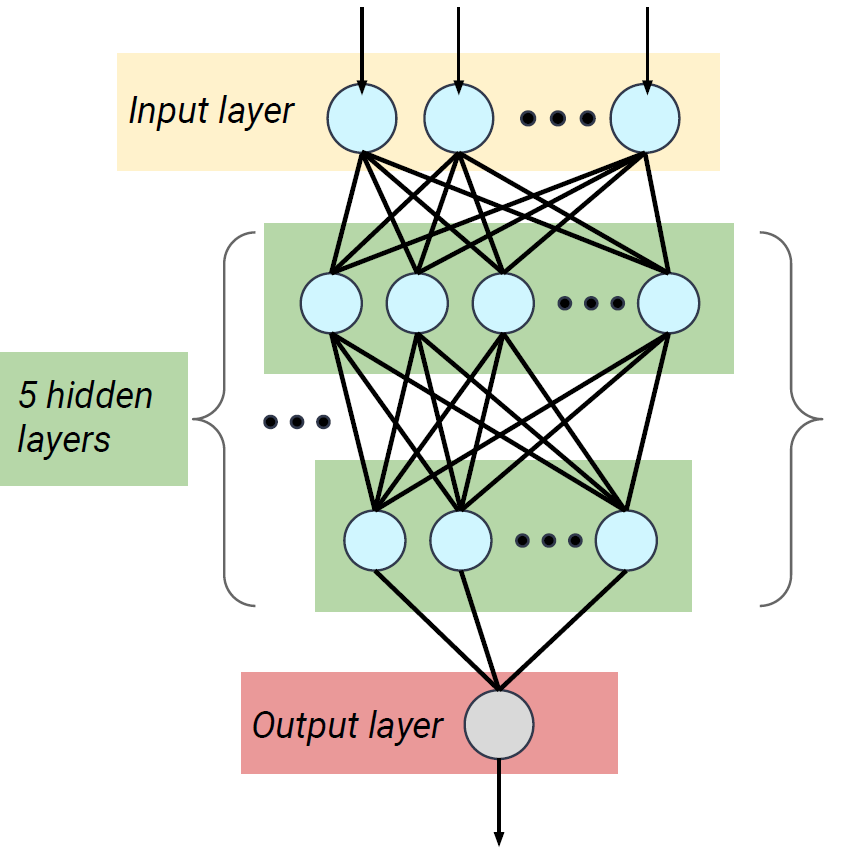
\includegraphics[width=0.55\textwidth]{figures/ml_dnn/DNNArchitecture.png}}
       \caption{Simplified DNN architecture visualisation.}
       \label{fig:DNNArchitecturePic}
\end{figure}

\begin{table}[ht]
    \centering
    \begin{tabular}{c|c|c|c}
     Layer(type) & Number of Neurons & Activation Functions & Regularizers\\
     \hline
     \hline
     Layer1(dense) & 64 & ReLu & L2\\
     Layer2(dense) & 32 & ReLu & L2\\
     Layer3(dense) & 32 & ReLu & L2\\
     Layer4(dense) & 32 & ReLu & L2\\
     Layer5(dense) & 16 & ReLu & L2\\
     Layer Out(dense) & 1 & Sigmoid & -\\
    \end{tabular}
    \caption{1-lepton DNN structure in merged and resolved signal regions.}
    \label{tab:1lepDNN layers}
\end{table}

\section{Input Variables and Feature Engineering}
\label{input_variables}

We assess the impact of input features on our DNNs using SHAP (SHapley Additive exPlanations), as introduced by Lundberg and Lee~\cite{LundbergLee2017}. SHAP quantifies the contribution of each feature to the deviation of a particular prediction from the average outcome across the dataset. This method provides a game theory-based interpretable approximation of complex neural networks, facilitating a deeper understanding of how individual features influence the model's predictions (DNN scores) for specific events. Employing SHAP values helps create a simplified yet faithful model that mirrors the original network's performance, making the decision-making process transparent and easier to interpret.

To optimize the DNN models, we use a backward feature elimination method, guided by SHAP value rankings, which is a recognized technique in feature selection. This approach involves systematically removing the least important input features, as determined by SHAP values, and then retraining the DNN models after each round to assess the impact of these eliminations on model performance. SHAP values are recalculated after each training session to ensure that the feature rankings are continuously updated. In the end, we retain 15 input features for the merged category and 17 for the resolved category, demonstrating tailored optimizations for each.
The final selection of input features for both categories is documented in Table~\ref{tab:1lepNN}, and their corresponding SHAP value rankings are illustrated in Figure~\ref{fig:1lepDNN_shap_rank}.

The term ``full system'' refers to variables associated with the entire set of signal jet(s), lepton(s), and tagging jets.
The boson centrality, $\xi(V)$, is defined as :  
\begin{equation} \label{eq:centr} \xi(V)  = min(\Delta\eta_{-},\Delta\eta_{+}) \end{equation} where $$\Delta\eta_{-} = min(\eta_{\Vlep},\eta_{\Vhad}) - min(\etajo,\etajt)$$ and  $$\Delta\eta_{+} = max(\etajo,\etajt) - max(\eta_{\Vlep},\eta_{\Vhad}) $$
Figures~\ref{fig:mer_inputs-part1}, \ref{fig:mer_inputs-part2}, \ref{fig:res_inputs-part1}, and \ref{fig:res_inputs-part2} display the distributions of input features within the SRs. The noticeable differences in distribution shapes between the signal and background MC samples, as shown in these figures, highlight the effectiveness of our feature selection process.

Figure~\ref{fig:ROCChecks} presents a comparison of the performance metrics for the initial and final DNN models in both the merged and resolved categories, demonstrating that both models achieve comparable levels of effectiveness. To better understand this comparison, 
we define signal efficiency and background rejection as follows:

\begin{equation}
\text{Signal Efficiency} = \frac{\text{Number of Signal events with DNN} > X}{\text{Total Number of Signal events}}
\end{equation}

\begin{equation}
\text{Background Rejection} = \frac{\text{Number of Background events with DNN} < X}{\text{Total Number of Background events}}.
\end{equation}

\begin{figure}[ht]
      \centering
       \subfloat[\emph{ROC Curve}]{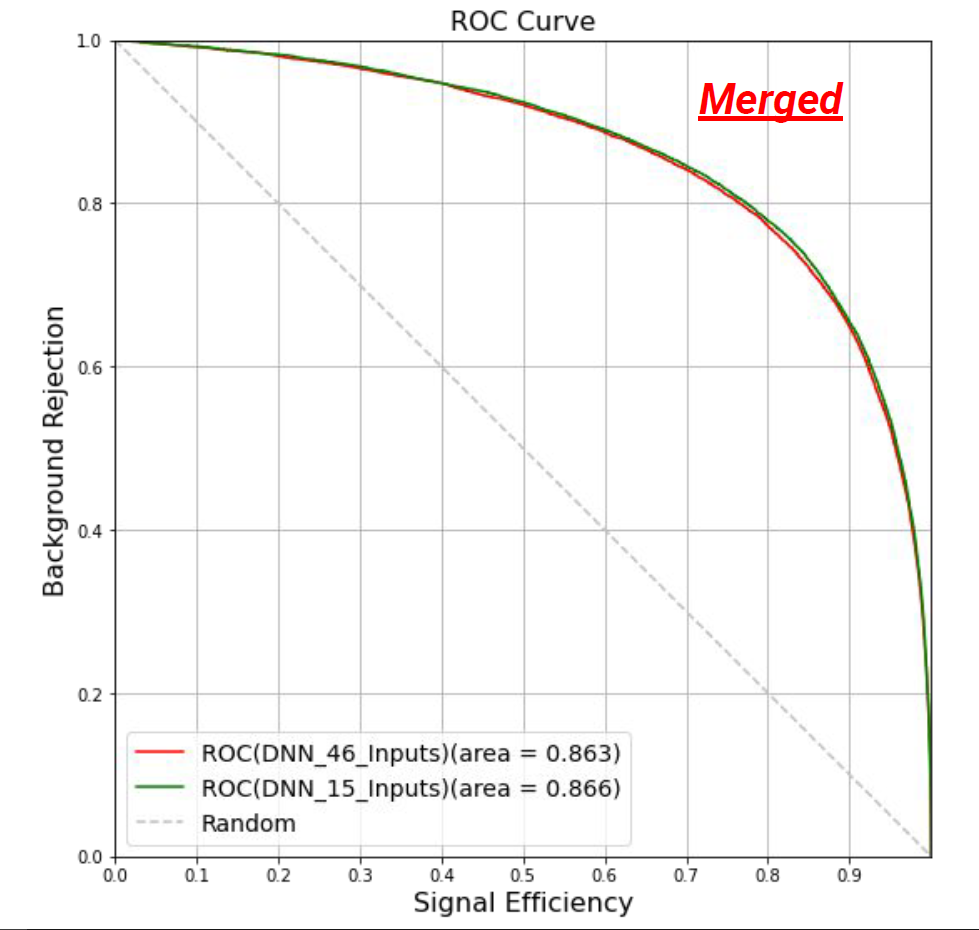
\includegraphics[width=0.4\textwidth]{figures/ml_dnn/ROCImpactMerged.png}}
       \subfloat[\emph{ROC Curve}]{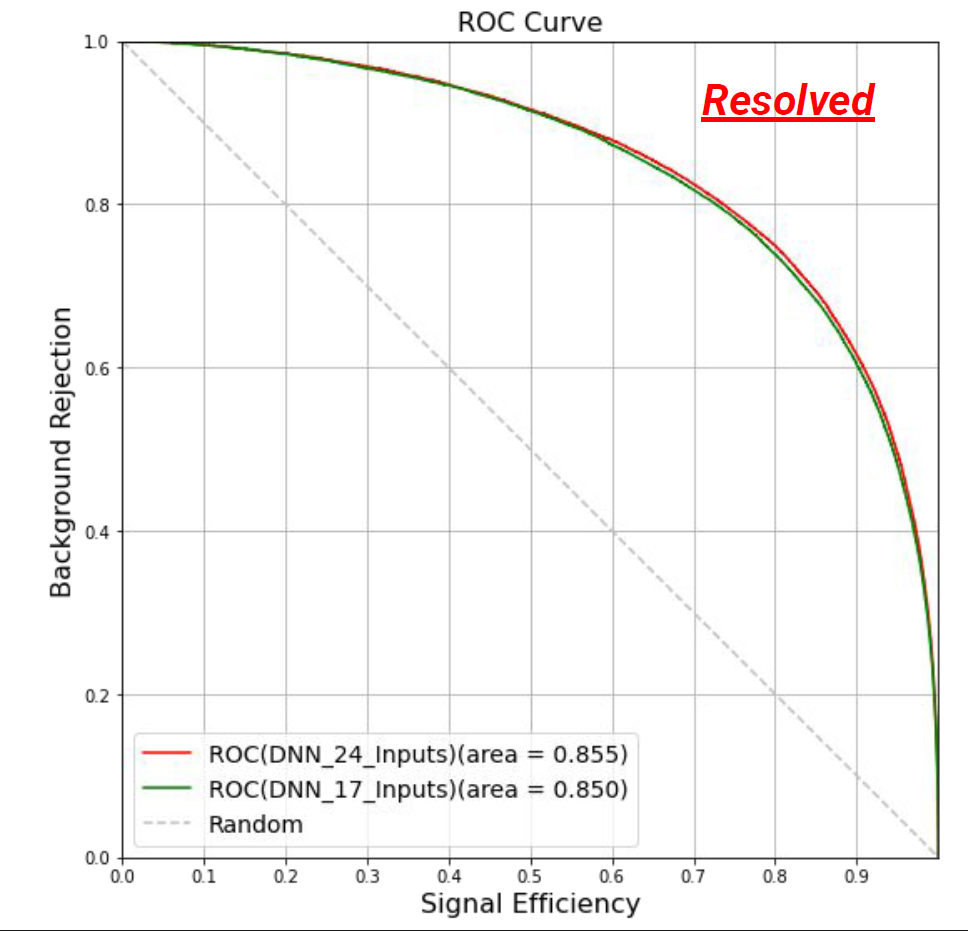
\includegraphics[width=0.4\textwidth]{figures/ml_dnn/ROCImpactRes.png}}
       \caption{ROC curves for the DNN models in the merged (a) and resolved (b) categories. Here, ``area'' refers to the AUC (Area Under the ROC Curve). The AUC values are computed to offer quantitative measures of performance.}
       \label{fig:ROCChecks}
\end{figure}

\begin{table}[ht]
    \centering
    \begin{tabular}{r|c|c}
     feature & merged & resolved\\
     \hline
     \hline
     signal jet(s) mass & $m(J^\text{sig})$ & $m(jj^\text{sig})$\\
     signal jet transverse momentum & $ - $ & $p_\text{T}(j^\text{sig}_\text{lead})$ and  $p_\text{T}(j^\text{sig}_\text{sublead})$\\
     signal jet width & $ - $ & $W(j^\text{sig}_\text{lead})$ and  $W(j^\text{sig}_\text{sublead})$\\
     dijet(signal jet) transverse momentum & $ - $ & $p_\text{T}(jj^\text{sig})$\\
     number of tracks associated to the signal jet(s) & $N_\text{trk}(J^\text{sig})$ & -\\
     multiplicity of B-tagged jets & $N(j^\text{B-tagged})$ & -\\
     multiplicity of forward jets & $N(j^\text{forward})$ & -\\
     multiplicity of track jets & - & $N(j^\text{track})$\\
     diboson mass & $m(V^\text{had}V^\text{lep})$ & $ - $\\
     leading tagging jet mass & $m(j^\text{tag}_\text{lead})$ & $ - $\\
     full system mass & $ - $ & $m(V^\text{had}V^\text{lep}+jj^\text{tag})$\\
     tagging jet transverse momentum & $p_\text{T}(j^\text{tag}_\text{sublead})$ & $p_\text{T}(j^\text{tag}_\text{lead})$ and $p_\text{T}(j^\text{tag}_\text{sublead})$\\
     tagging jet width & $W(j^\text{tag}_\text{lead})$ and $W(j^\text{tag}_\text{sublead})$  & $ - $\\
     boson centrality & $\xi(V)$ & $ - $\\
     pseudo-rapidity of tagging jets & - & $\eta(j^\text{tag}_\text{lead})$ and $ \eta(j^\text{tag}_\text{sublead})$\\
     pseudo-rapidity of lepton & - & $\eta(l)$\\
     lepton transverse momentum & $p_\text{T}(l)$ & -\\
%%%     jets multiplicity & \multicolumn{2}{c}{$N(j)$}\\
     number of tracks associated to the tagging jets & $N_\text{trk}(j^\text{tag}_\text{lead})$ and $N_\text{trk}(j^\text{tag}_\text{sublead})$ & -\\
     jets multiplicity & \multicolumn{2}{c}{$N(j)$}\\
     tagging jets mass & \multicolumn{2}{c}{$m(jj^\text{tag})$}\\
     tagging jet separation & \multicolumn{2}{c}{$\Delta\eta(j^\text{tag}_\text{lead},j^\text{tag}_\text{sublead})$}\\
     lepton energy & \multicolumn{2}{c}{$E_{\ell}$}\\
    \end{tabular}
    \caption{Input variables for the 1-lepton DNN in merged and resolved signal regions.}
    \label{tab:1lepNN}
\end{table}

\begin{figure}[ht]
      \centering
       \subfloat[\emph{Rankings Merged}]{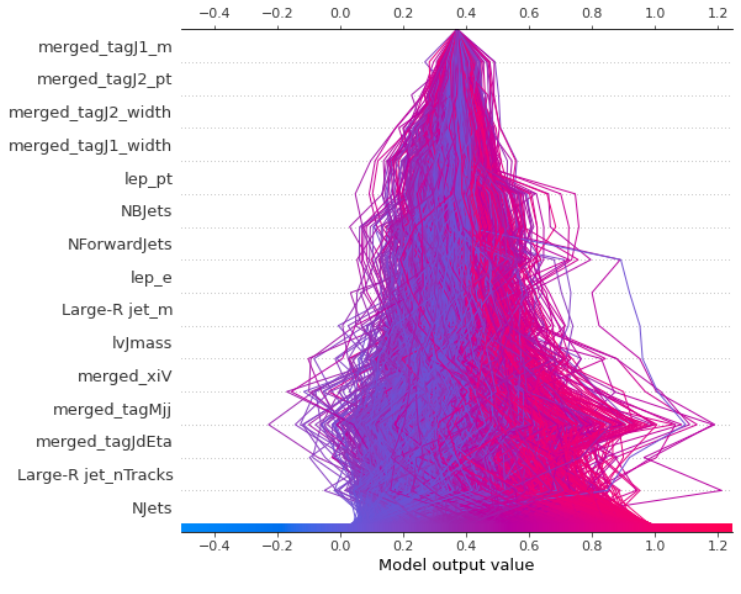
\includegraphics[width=0.4\textwidth]{figures/ml_dnn/rankings/decision_plot_mer.PNG}}
       \hspace{5mm}
       \subfloat[\emph{Rankings Resolved}]{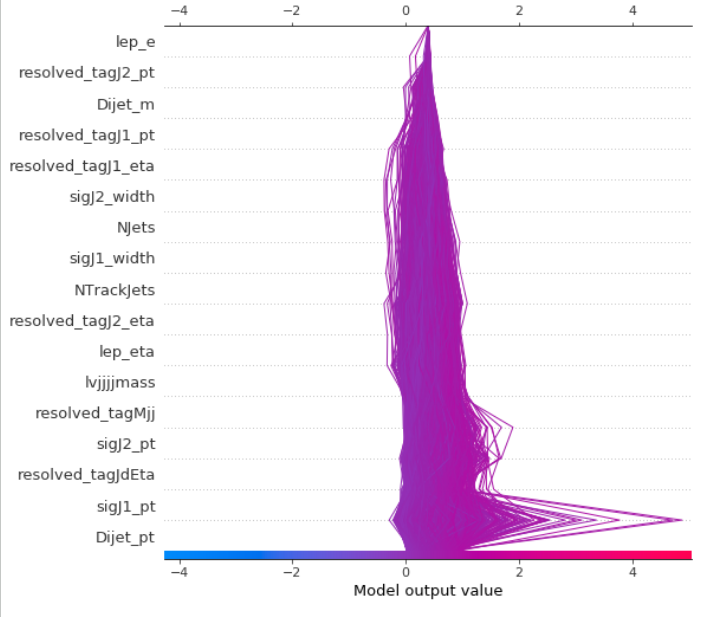
\includegraphics[width=0.4\textwidth]{figures/ml_dnn/rankings/decision_plot_res.PNG}}
       \caption{SHAP value rankings of input variables for both merged and resolved regimes; variables with lower impact appear at the top.}
       \label{fig:1lepDNN_shap_rank}
\end{figure}

\begin{figure}[ht]
 \centering
  % Row 1
  \subfloat[]{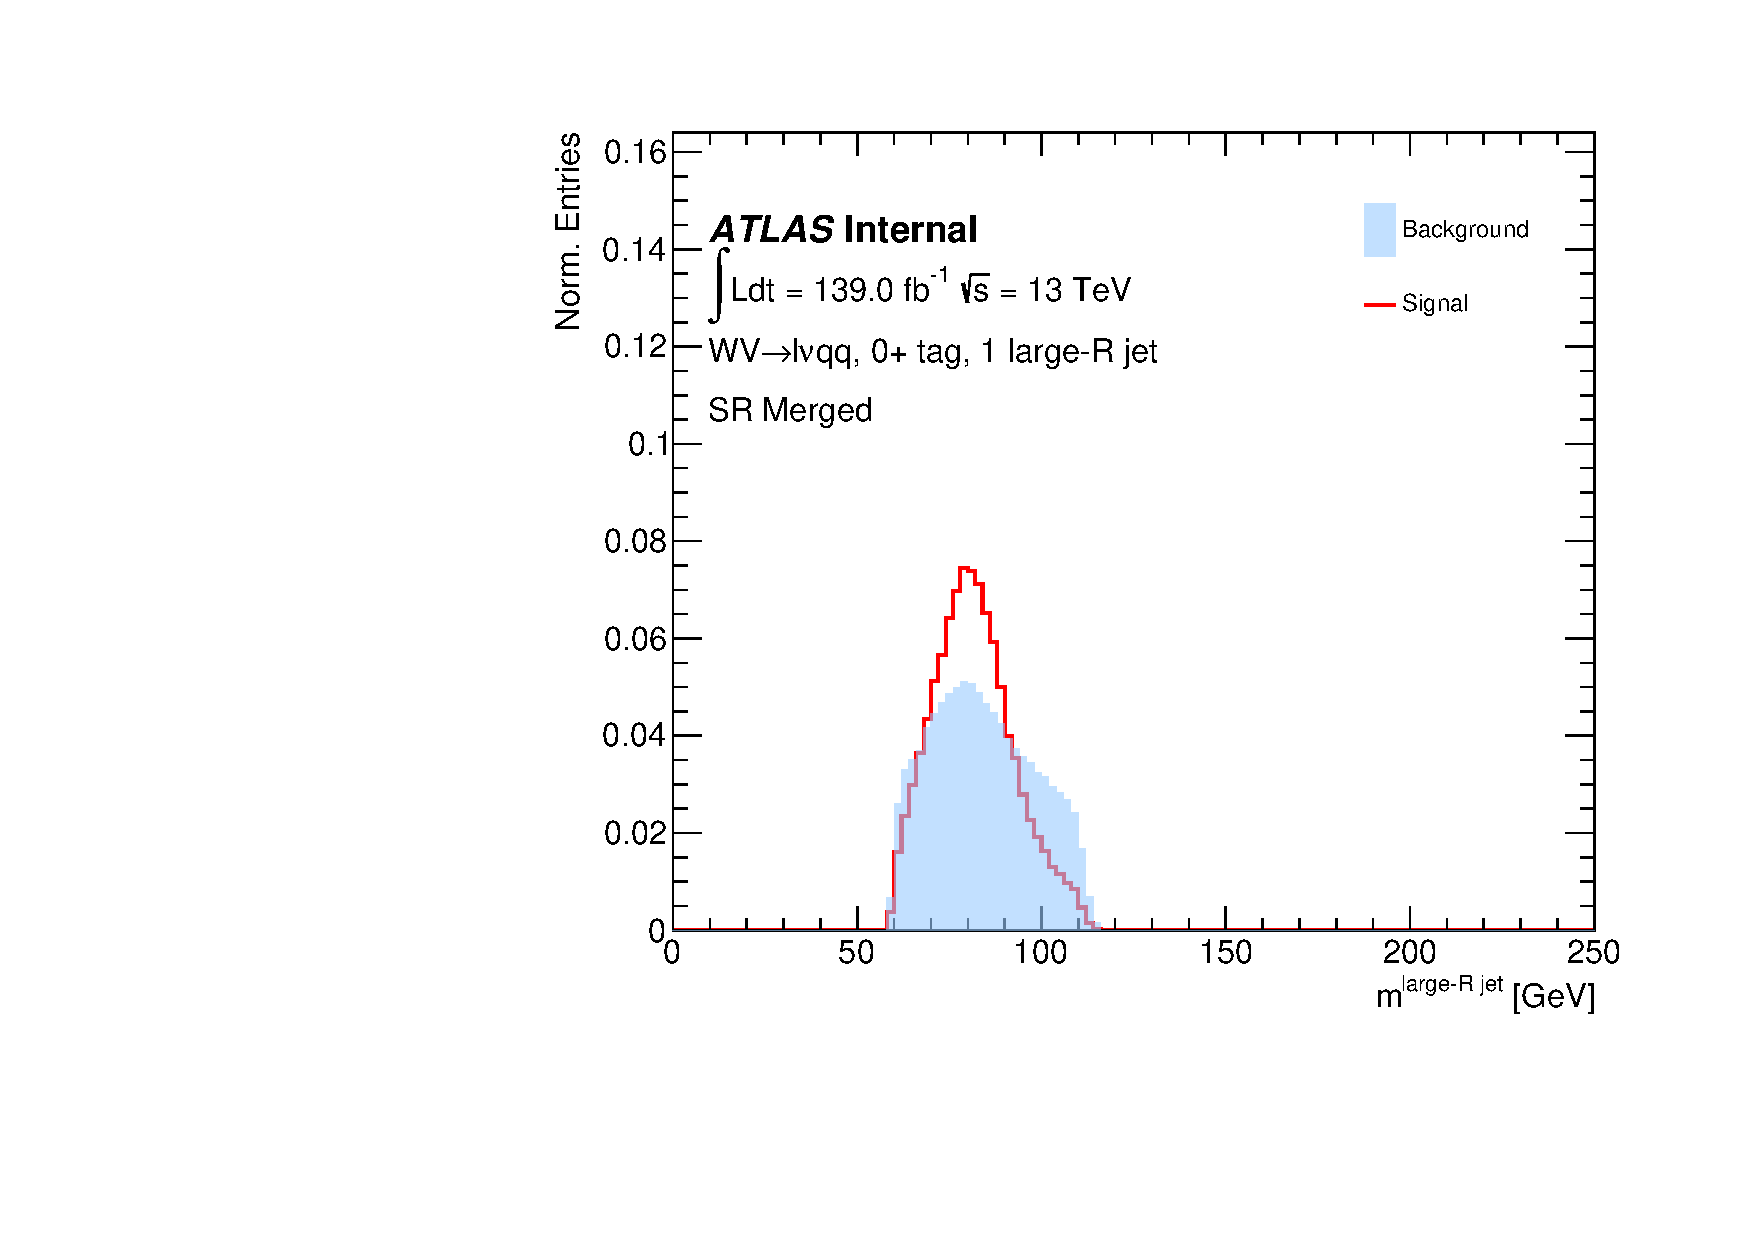
\includegraphics[width=0.3\textwidth]{figures/ml_dnn/variables/SR_Mer/norm_plot_fatJ_m.pdf}}\quad
  \subfloat[]{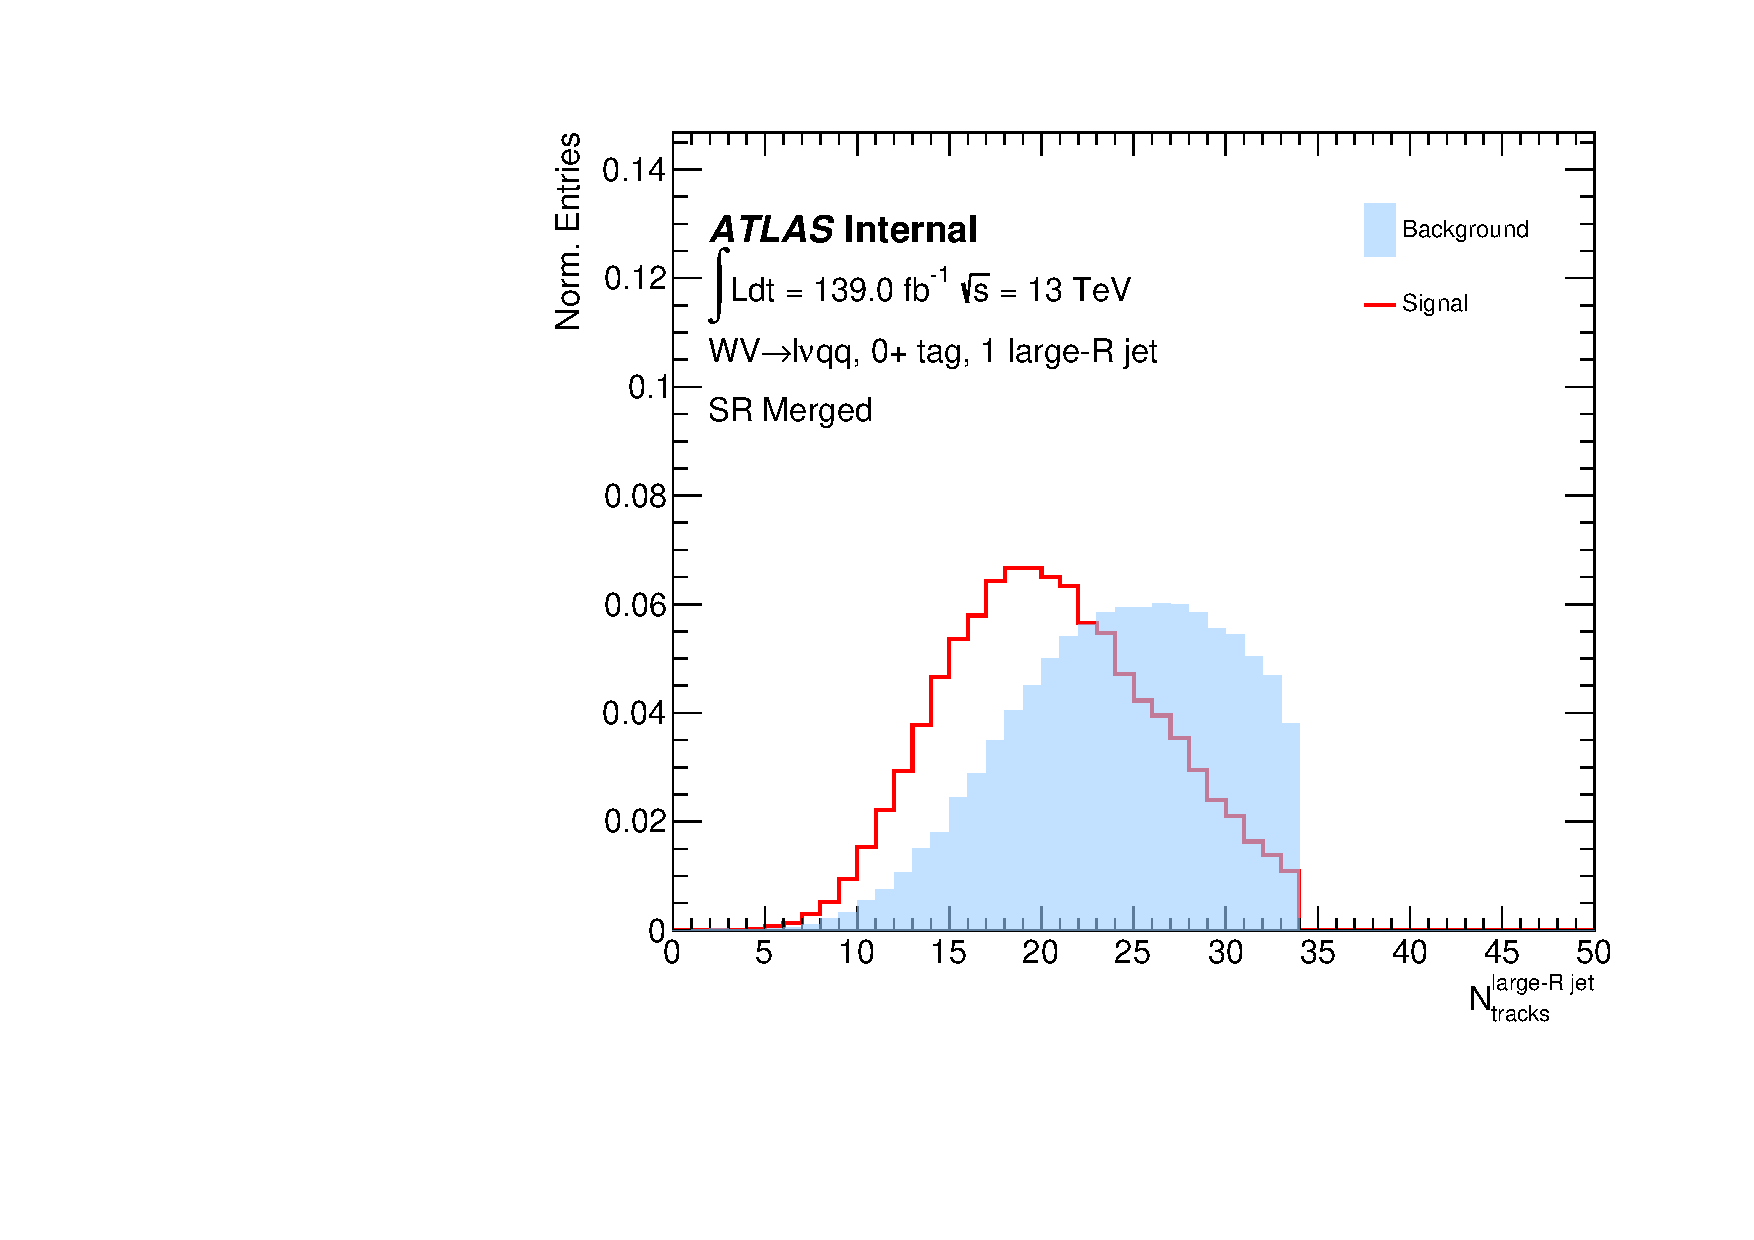
\includegraphics[width=0.3\textwidth]{figures/ml_dnn/variables/SR_Mer/norm_plot_fatJ_nTracks.pdf}}\quad
  \subfloat[]{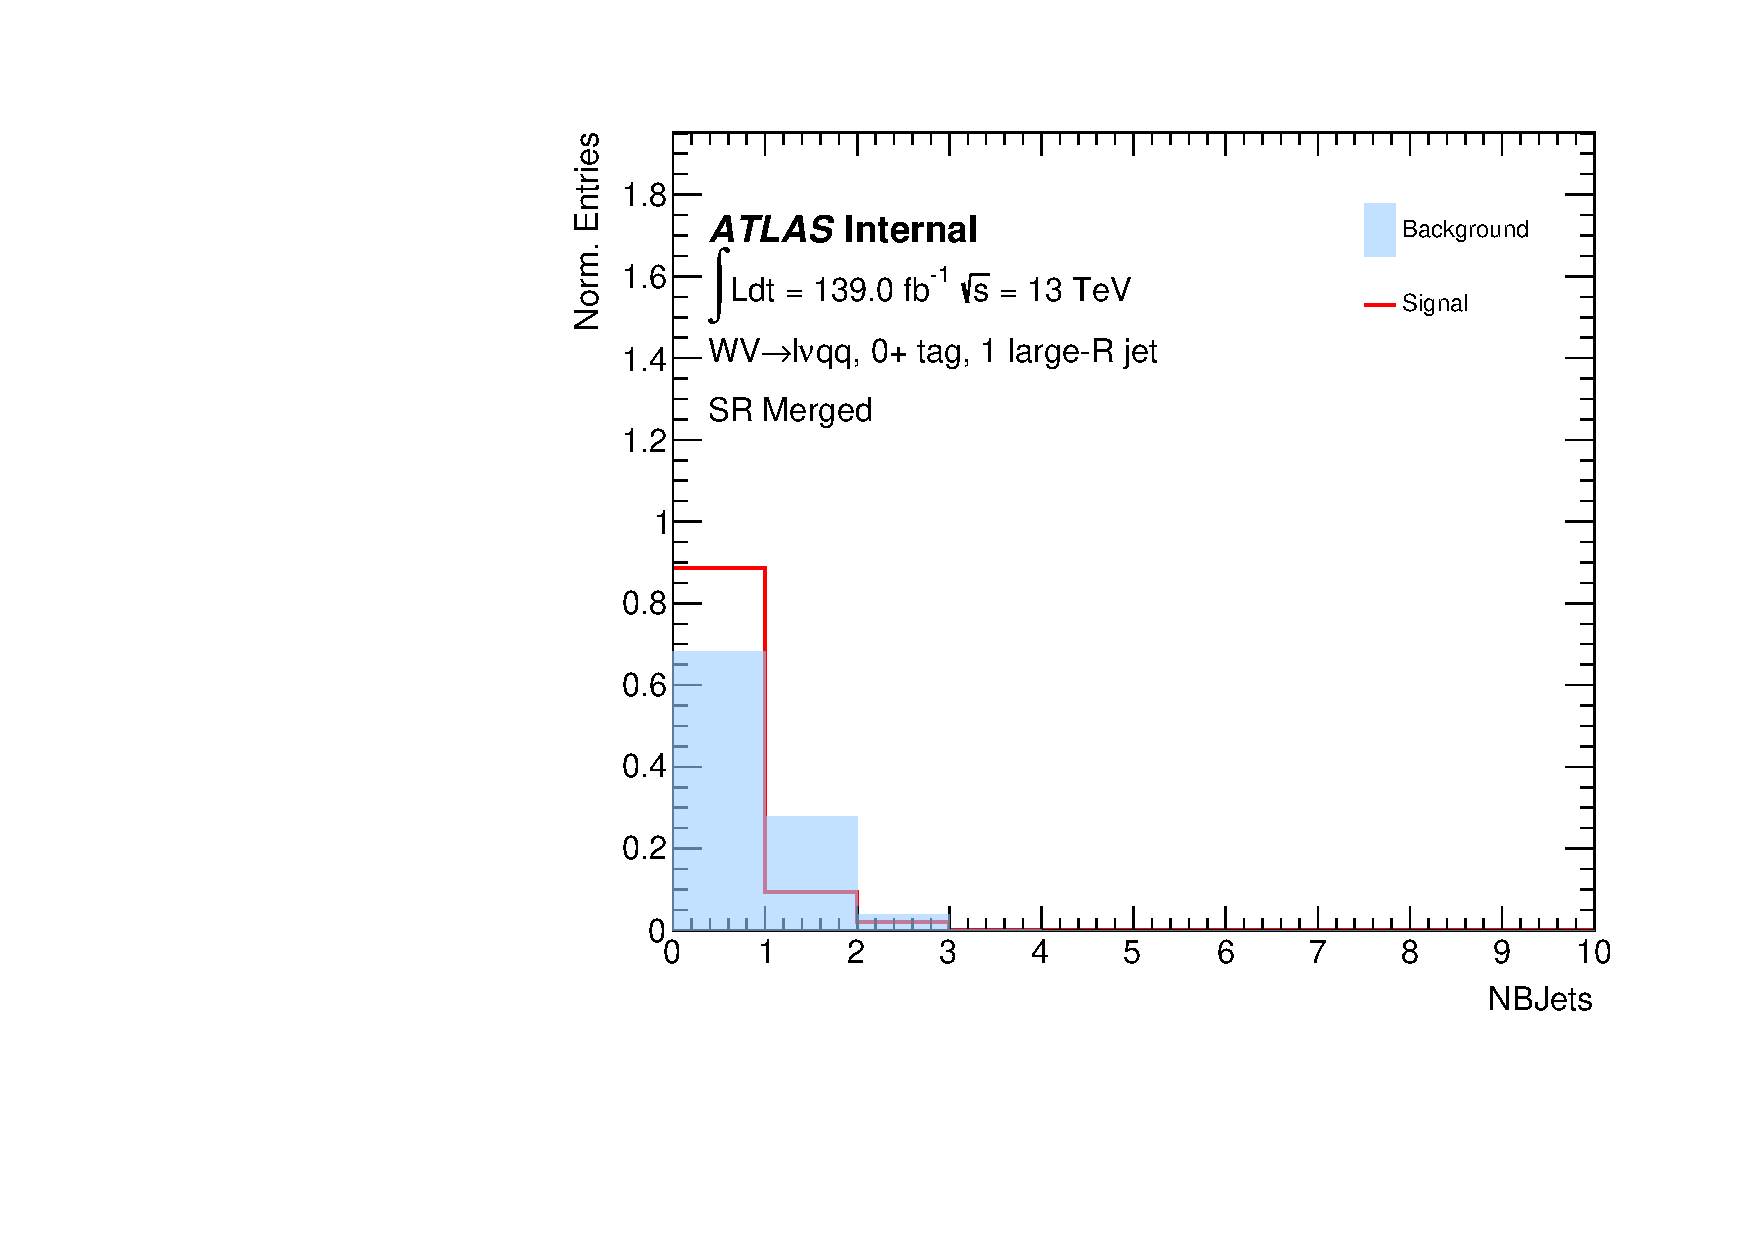
\includegraphics[width=0.3\textwidth]{figures/ml_dnn/variables/SR_Mer/norm_plot_NBJets.pdf}}

  % Row 2
  \subfloat[]{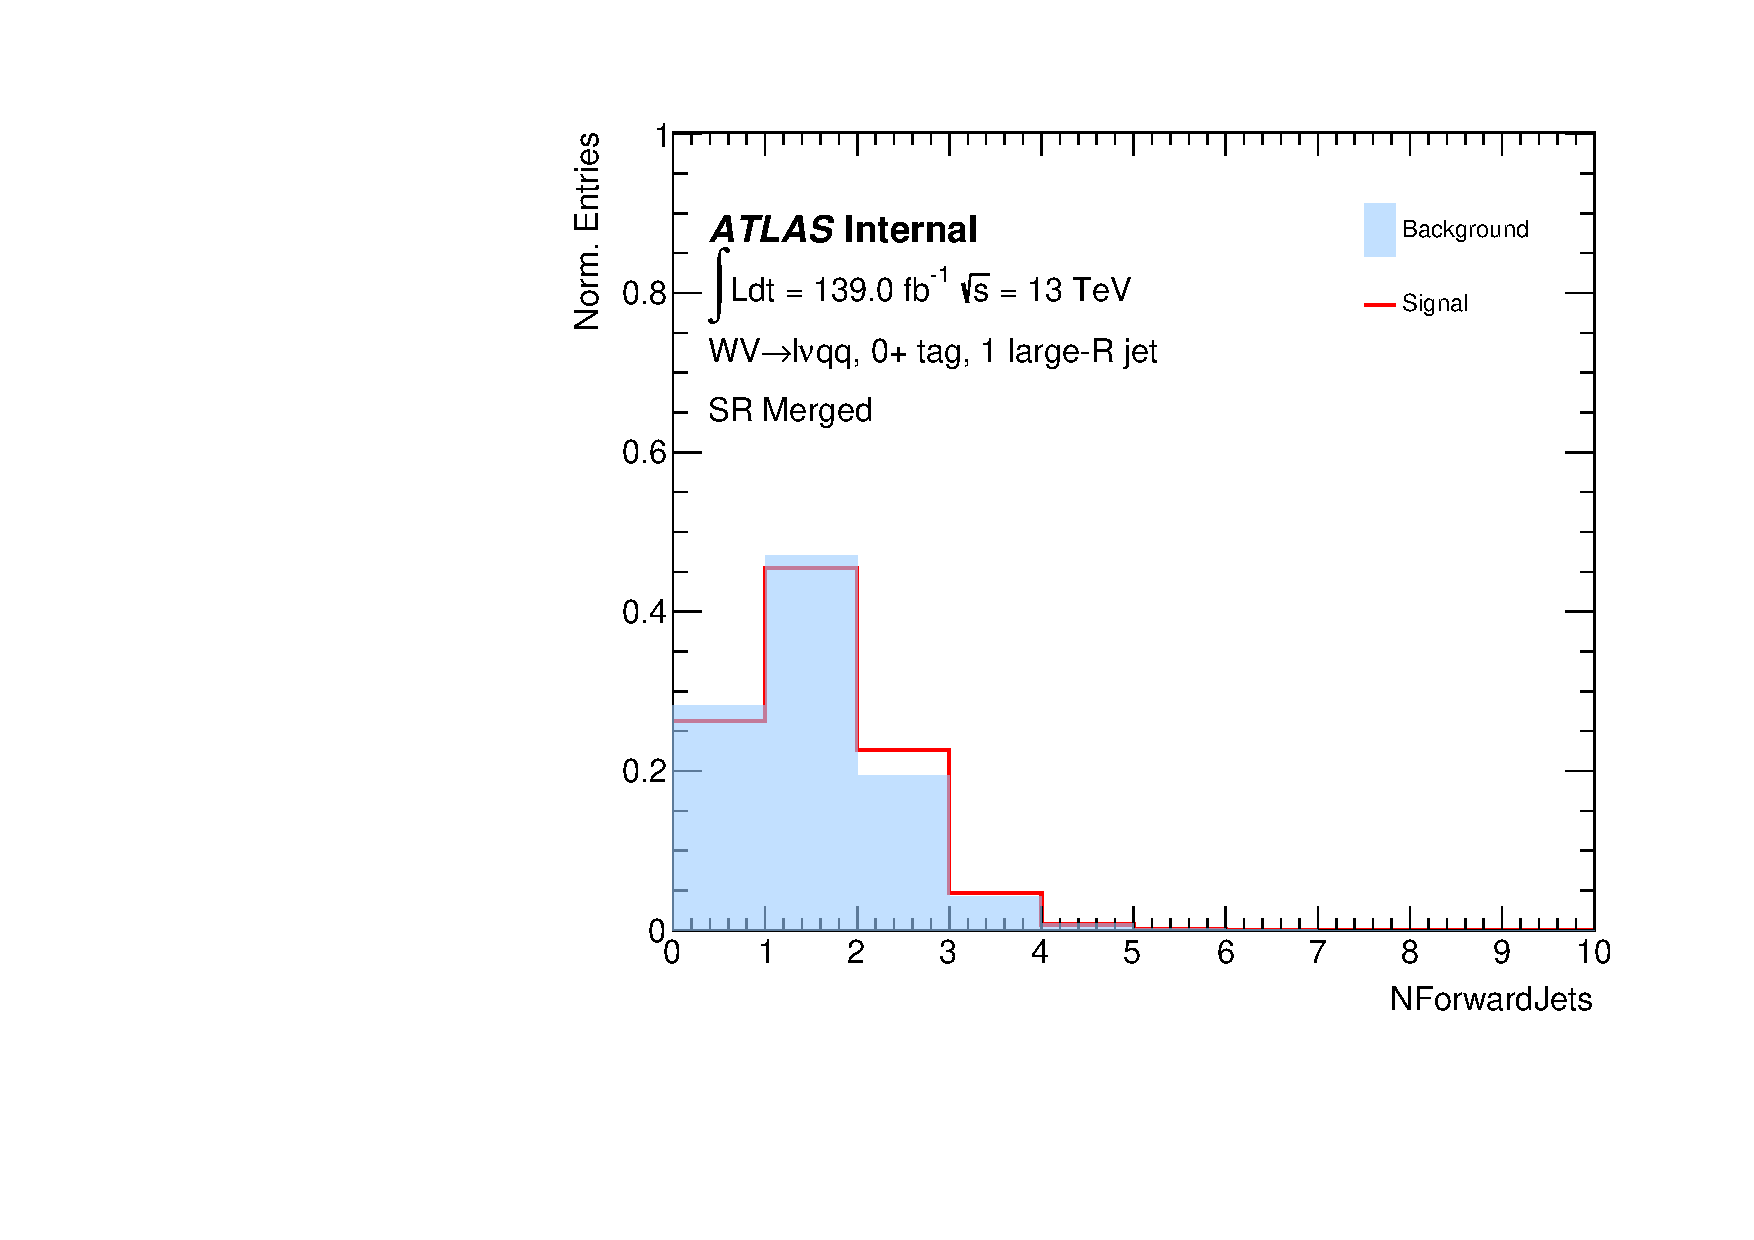
\includegraphics[width=0.3\textwidth]{figures/ml_dnn/variables/SR_Mer/norm_plot_NForwardJets.pdf}}\quad
  \subfloat[]{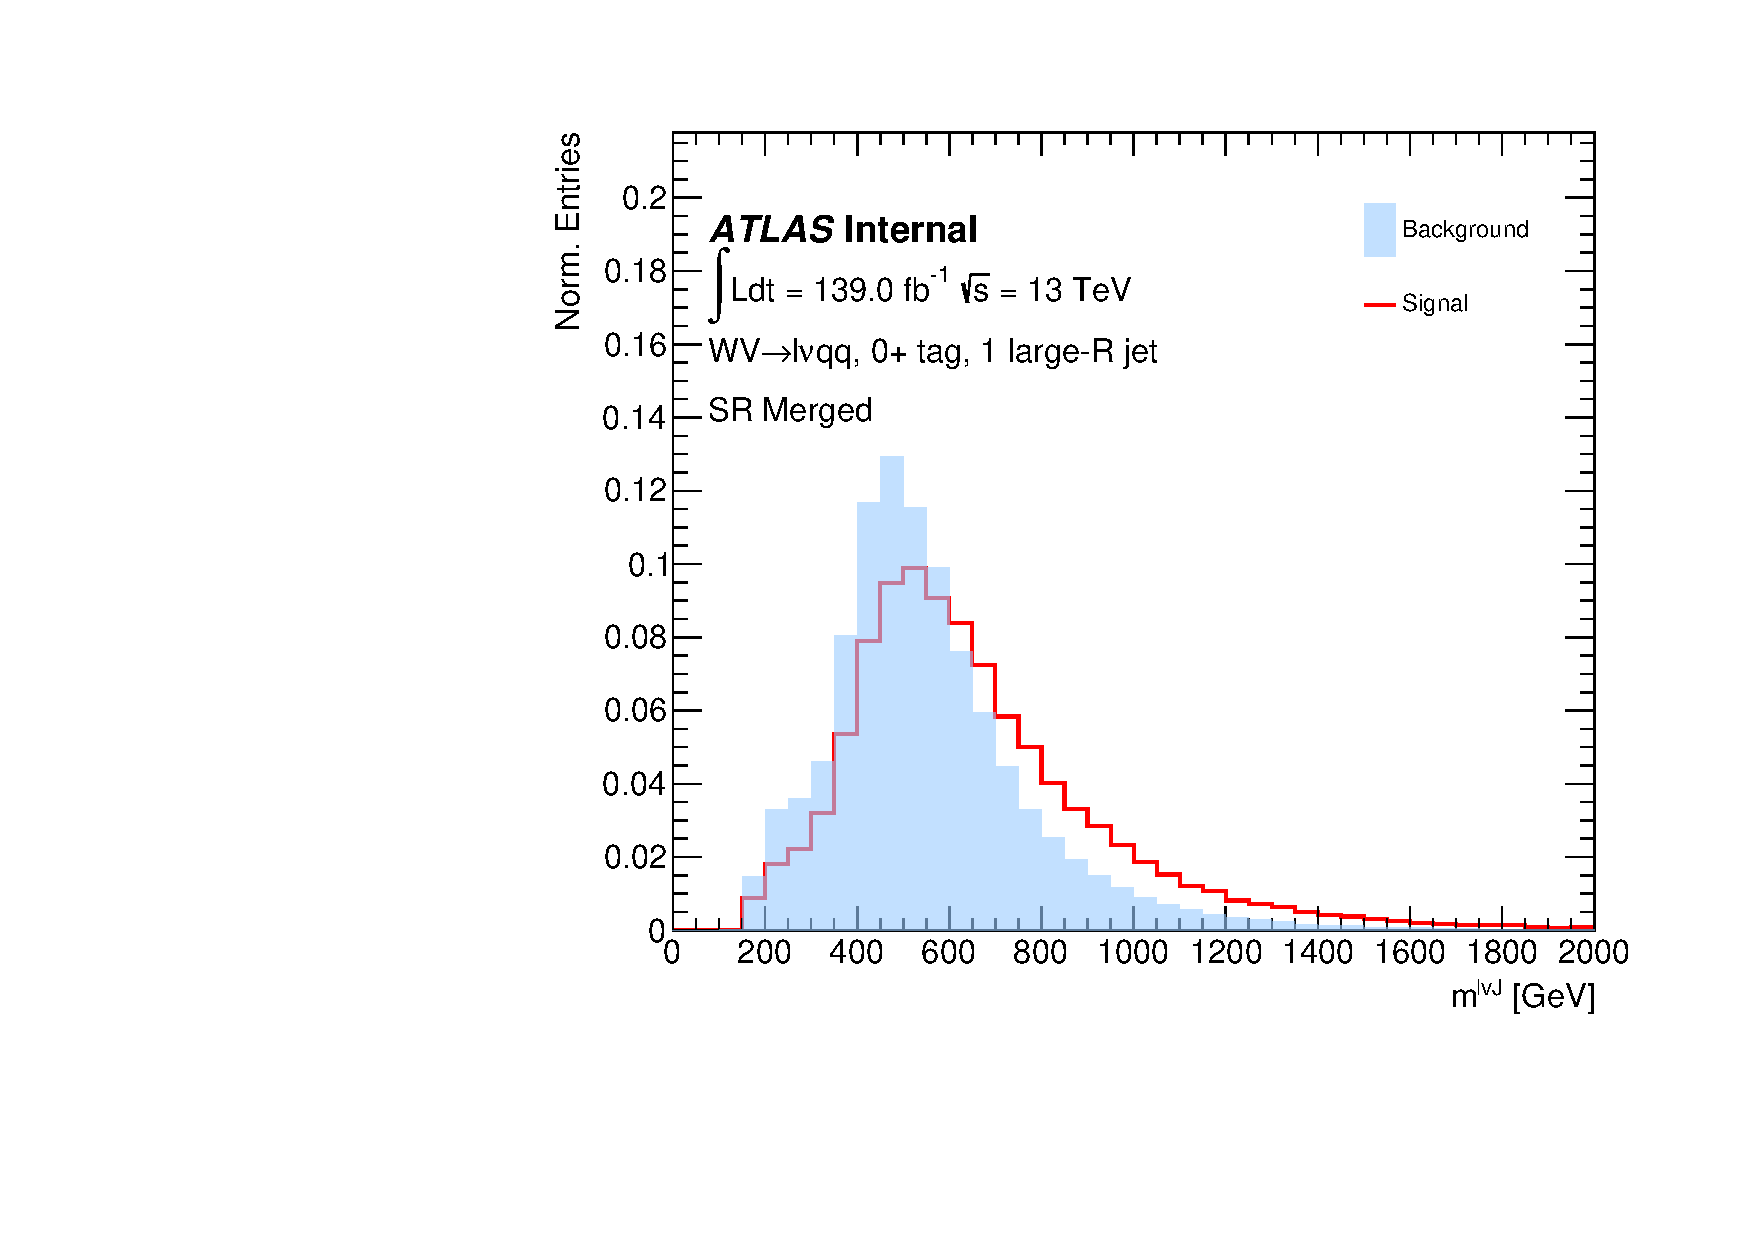
\includegraphics[width=0.3\textwidth]{figures/ml_dnn/variables/SR_Mer/norm_plot_lvJmass.pdf}}\quad
  \subfloat[]{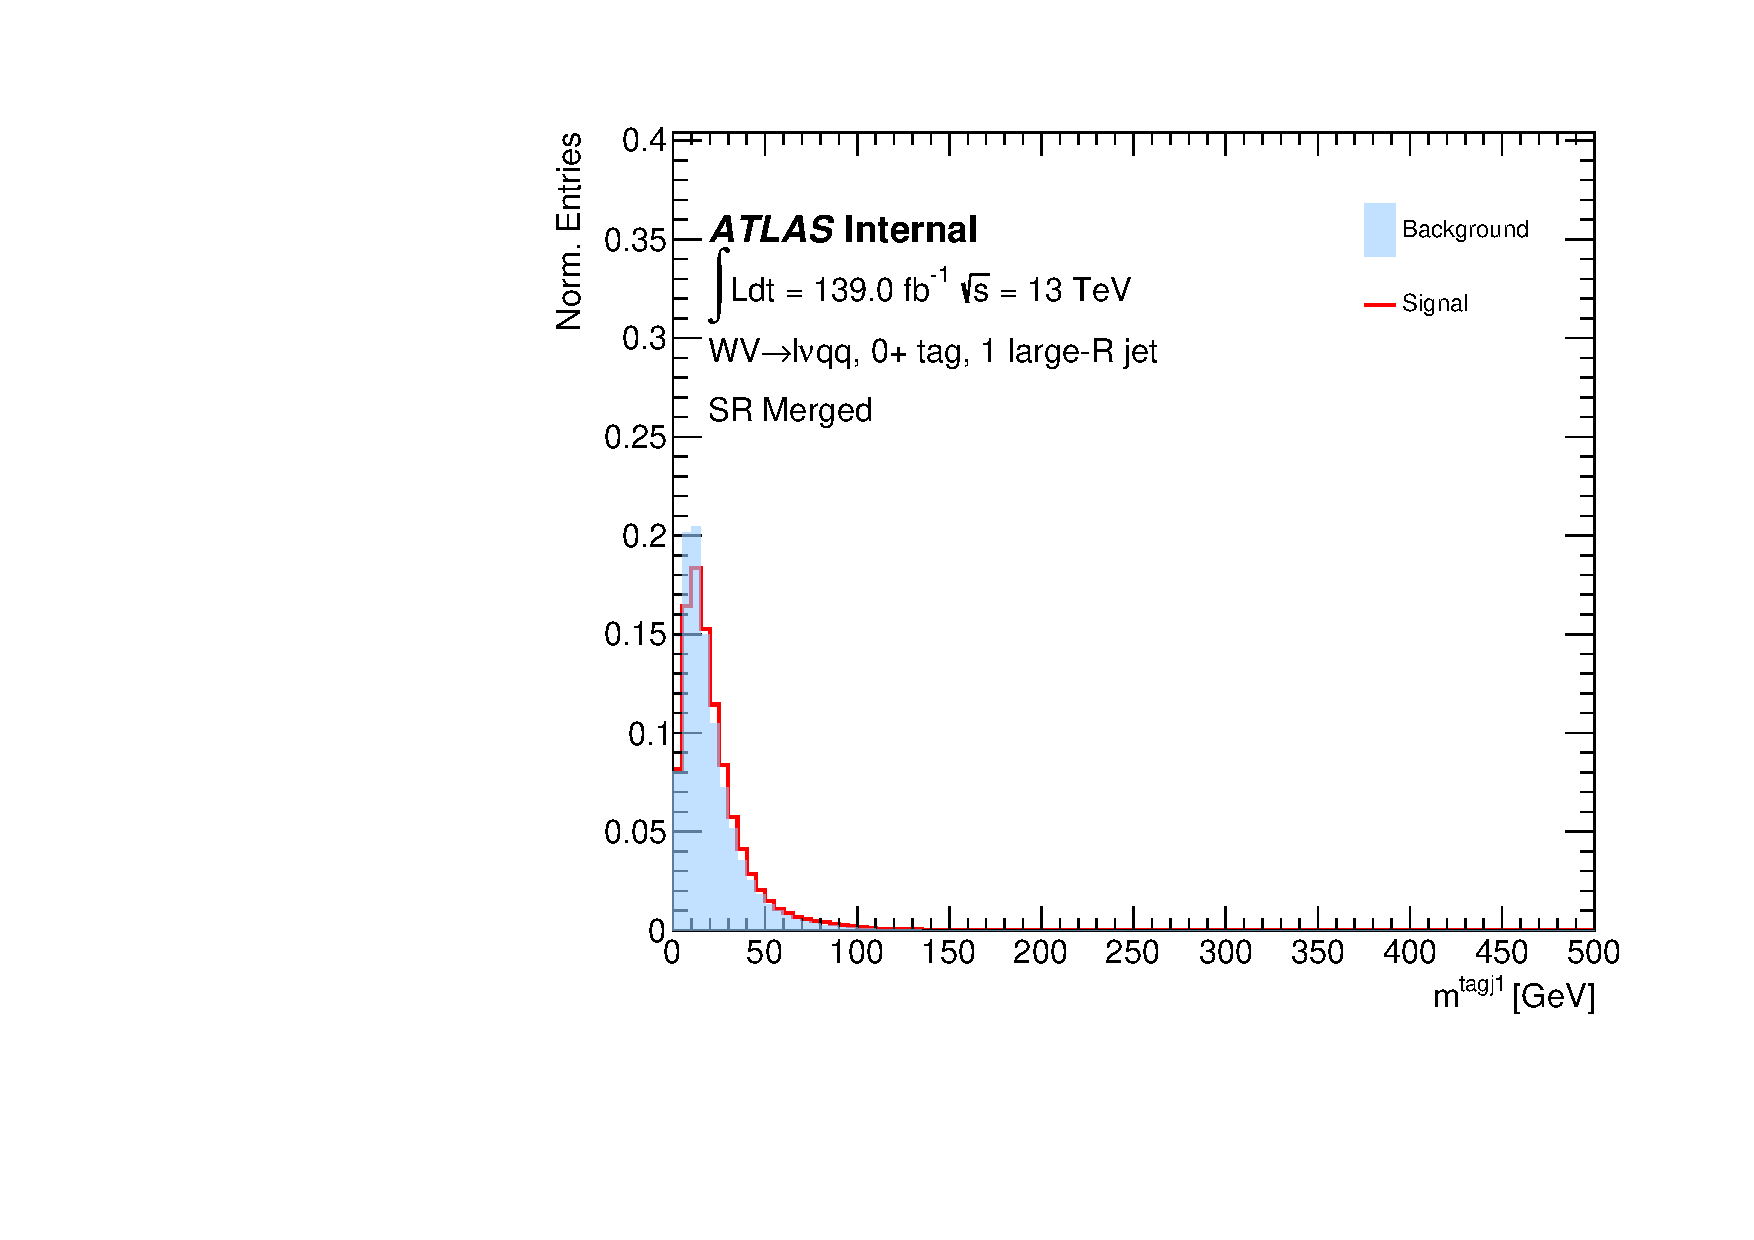
\includegraphics[width=0.3\textwidth]{figures/ml_dnn/variables/SR_Mer/norm_plot_merged_tagJ1_m.pdf}}

  % Row 3
%%  \subfloat[]{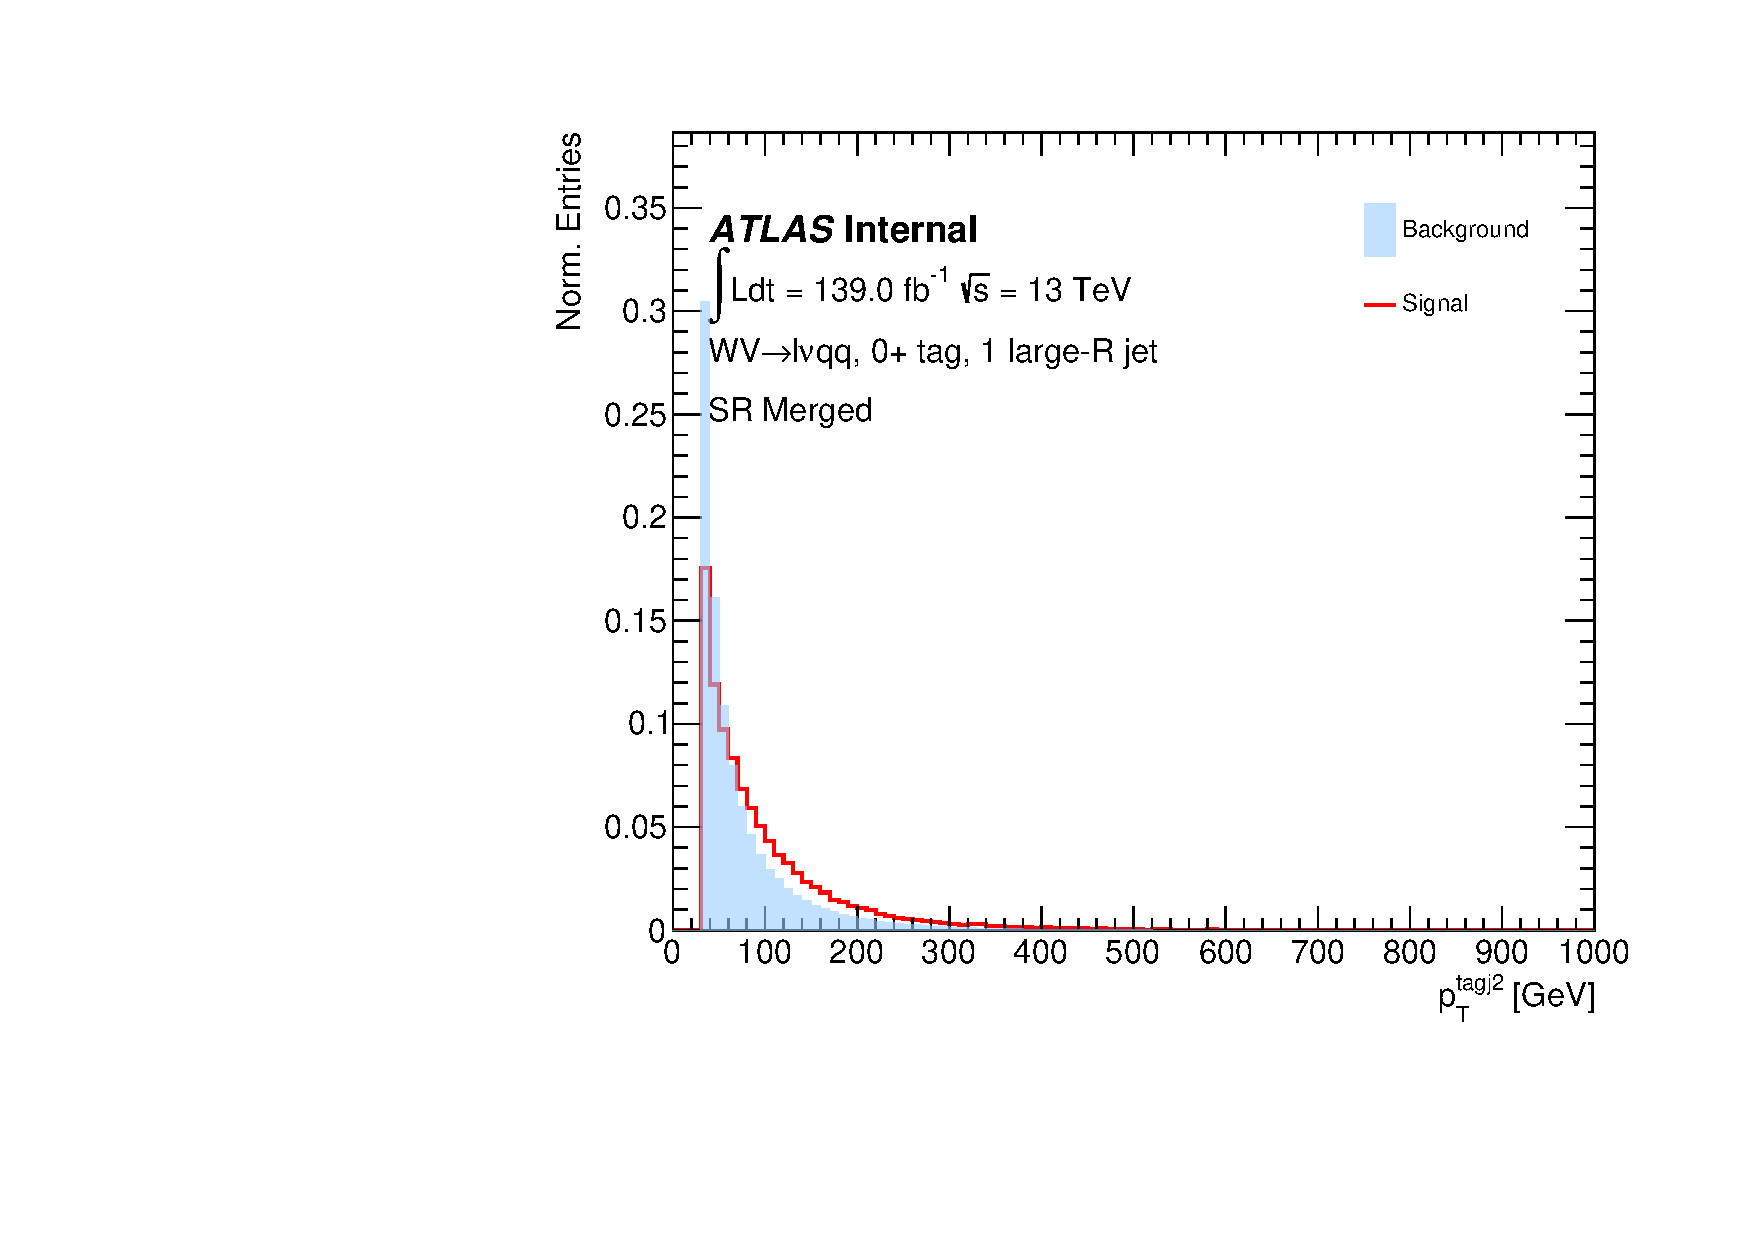
\includegraphics[width=0.3\textwidth]{figures/ml_dnn/variables/SR_Mer/norm_plot_merged_tagJ2_pt.pdf}}\quad
%%  \subfloat[]{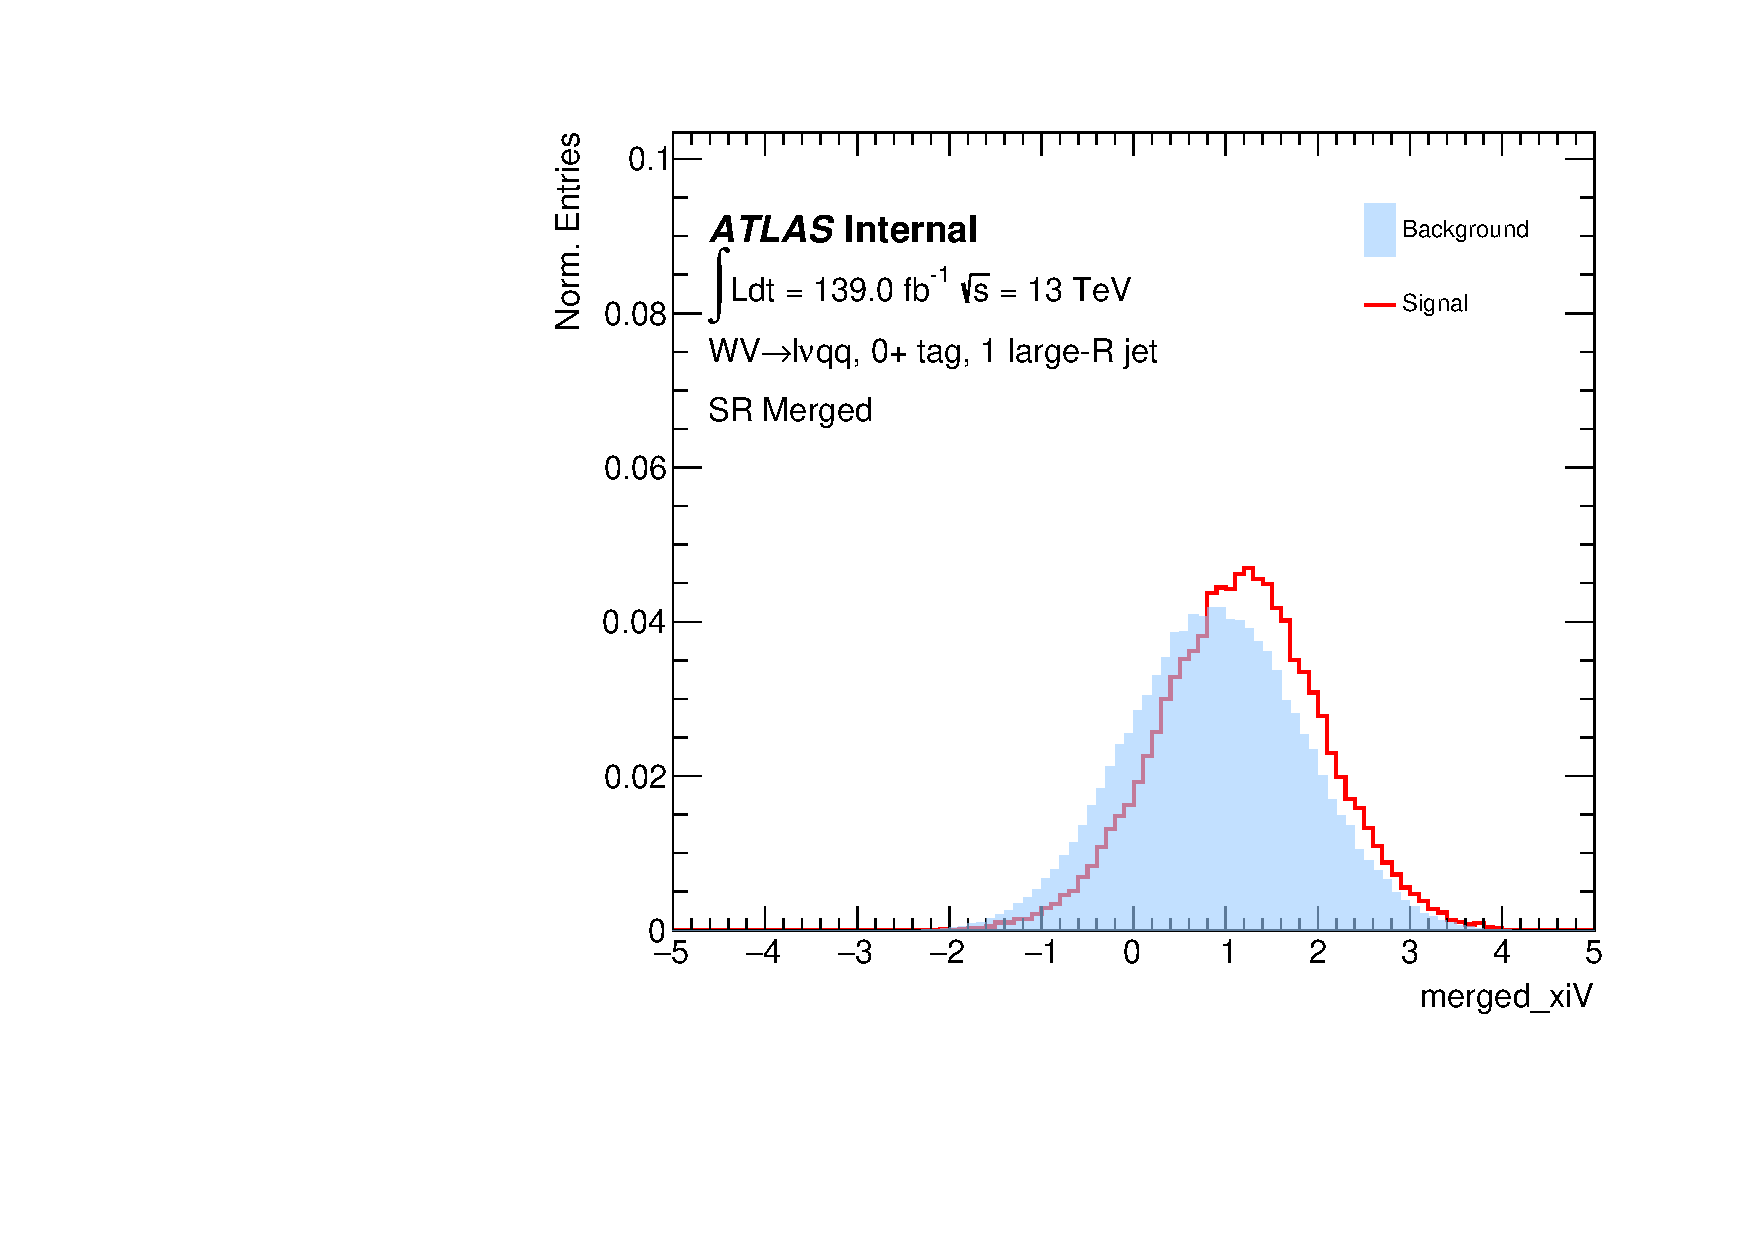
\includegraphics[width=0.3\textwidth]{figures/ml_dnn/variables/SR_Mer/norm_plot_merged_xiV.pdf}}\quad
%%  \subfloat[]{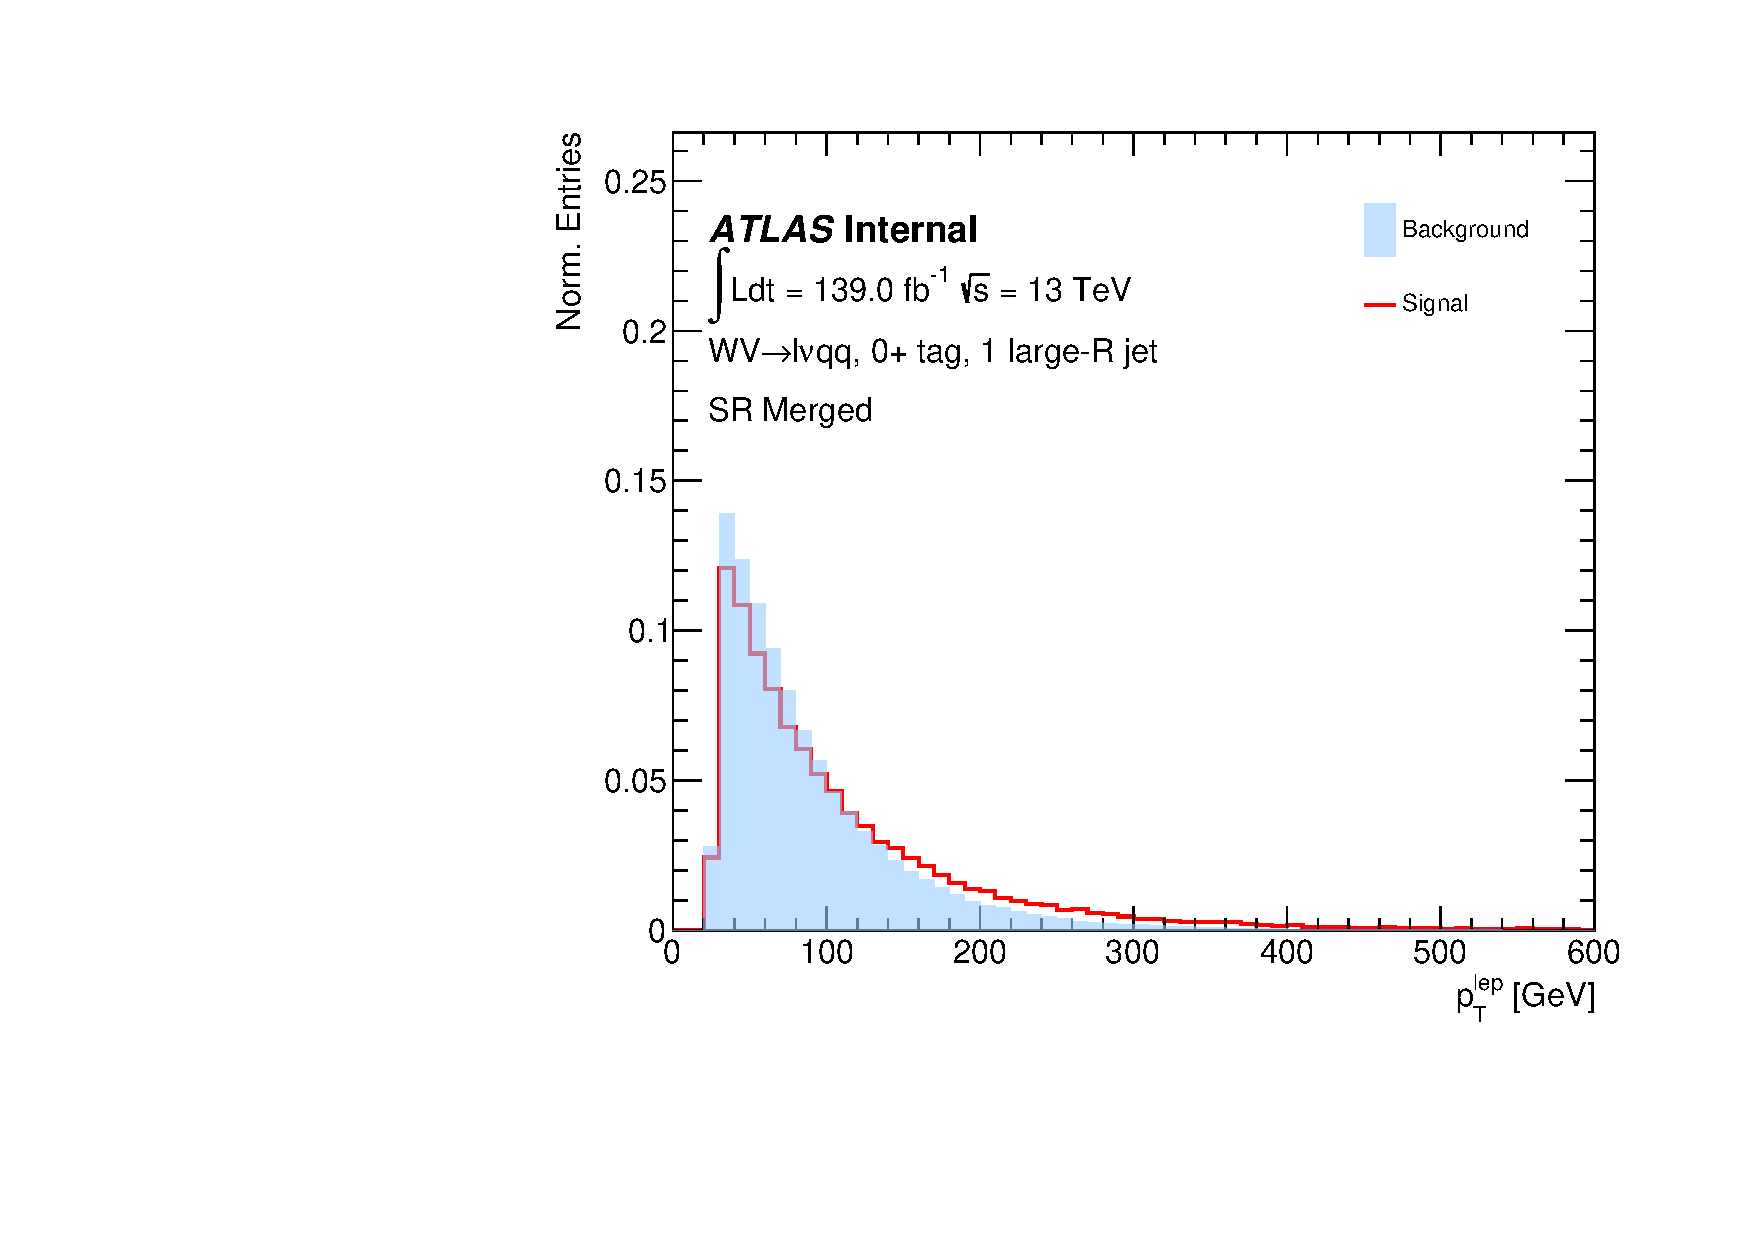
\includegraphics[width=0.3\textwidth]{figures/ml_dnn/variables/SR_Mer/norm_plot_lep_pt.pdf}}

 \caption{Distributions of input variables in the Merged SR (Continued on next page)}
 \label{fig:mer_inputs-part1}
\end{figure}

\begin{figure}[ht]
 \centering
  % Row 3
  \subfloat[]{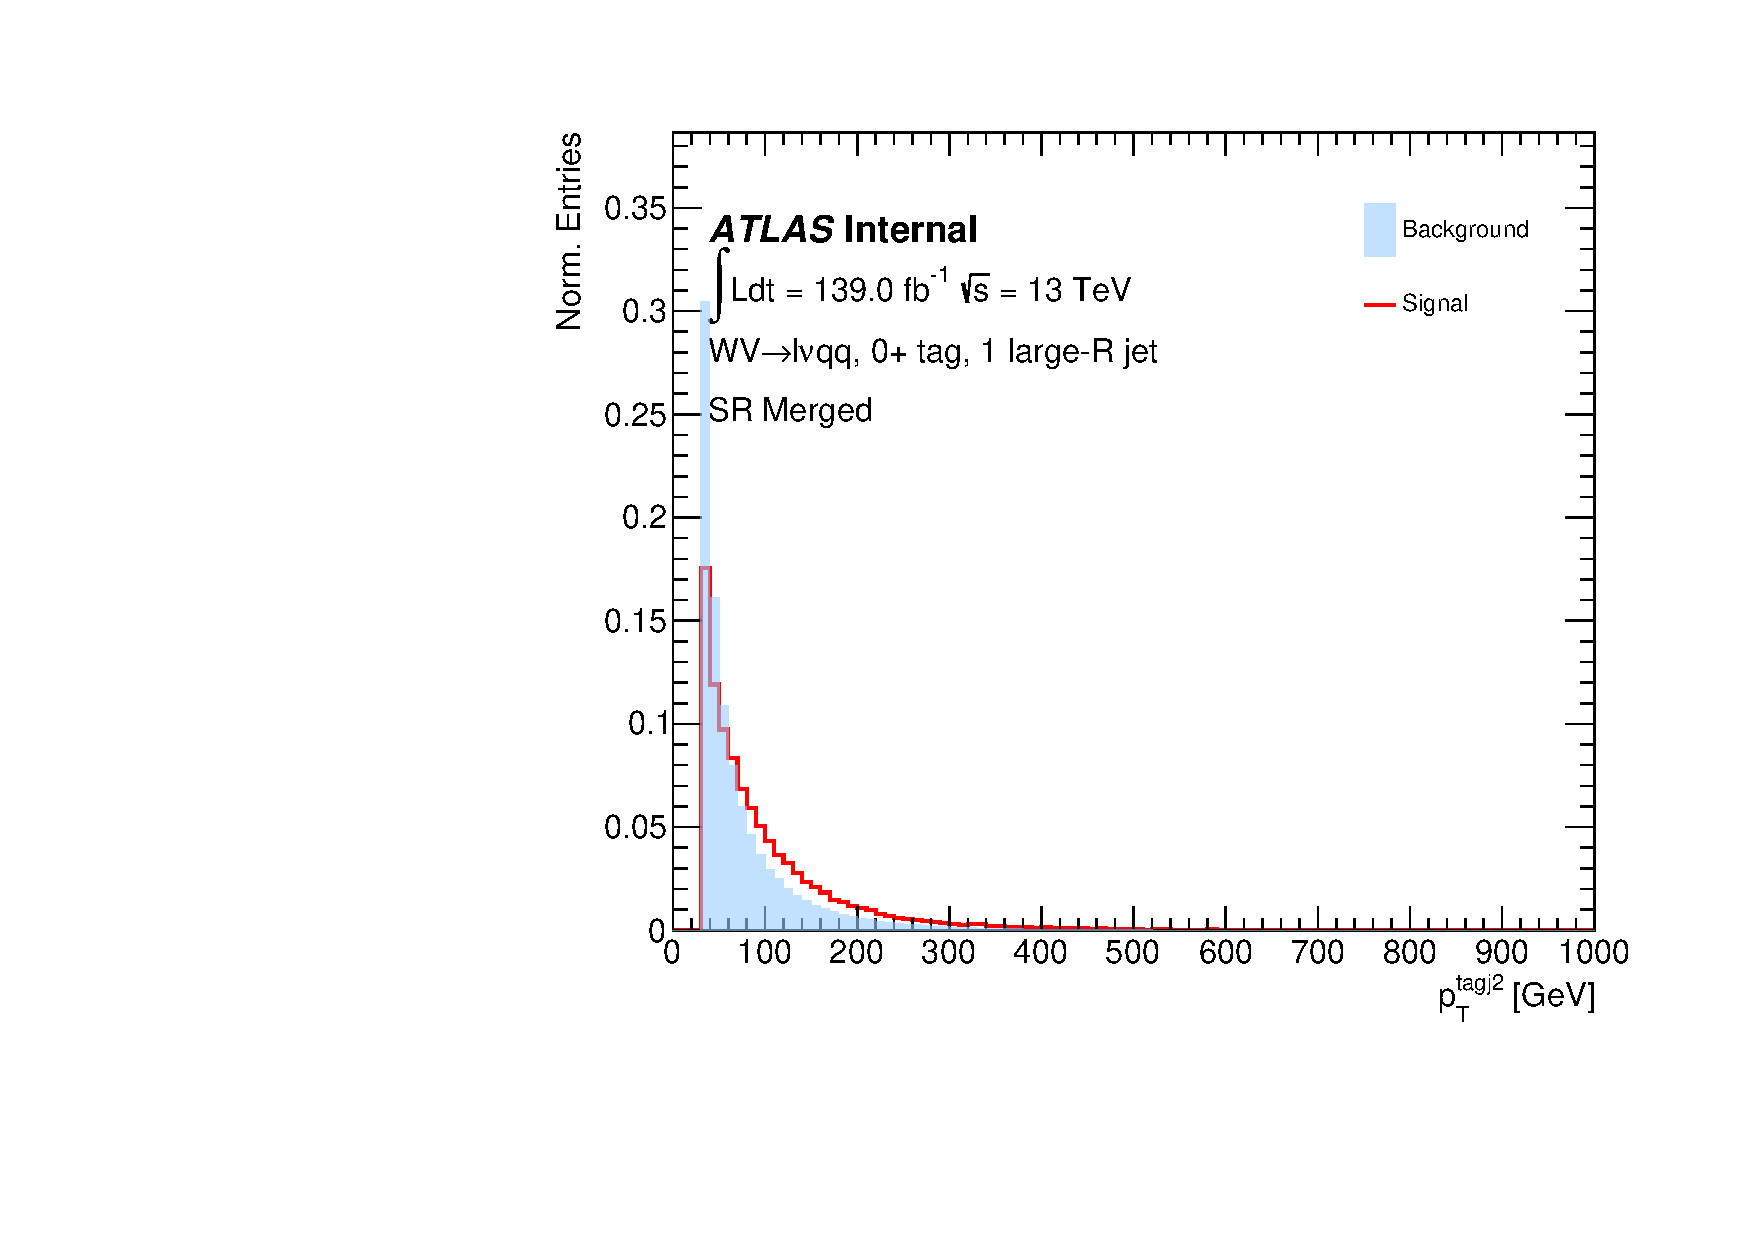
\includegraphics[width=0.3\textwidth]{figures/ml_dnn/variables/SR_Mer/norm_plot_merged_tagJ2_pt.pdf}}\quad
  \subfloat[]{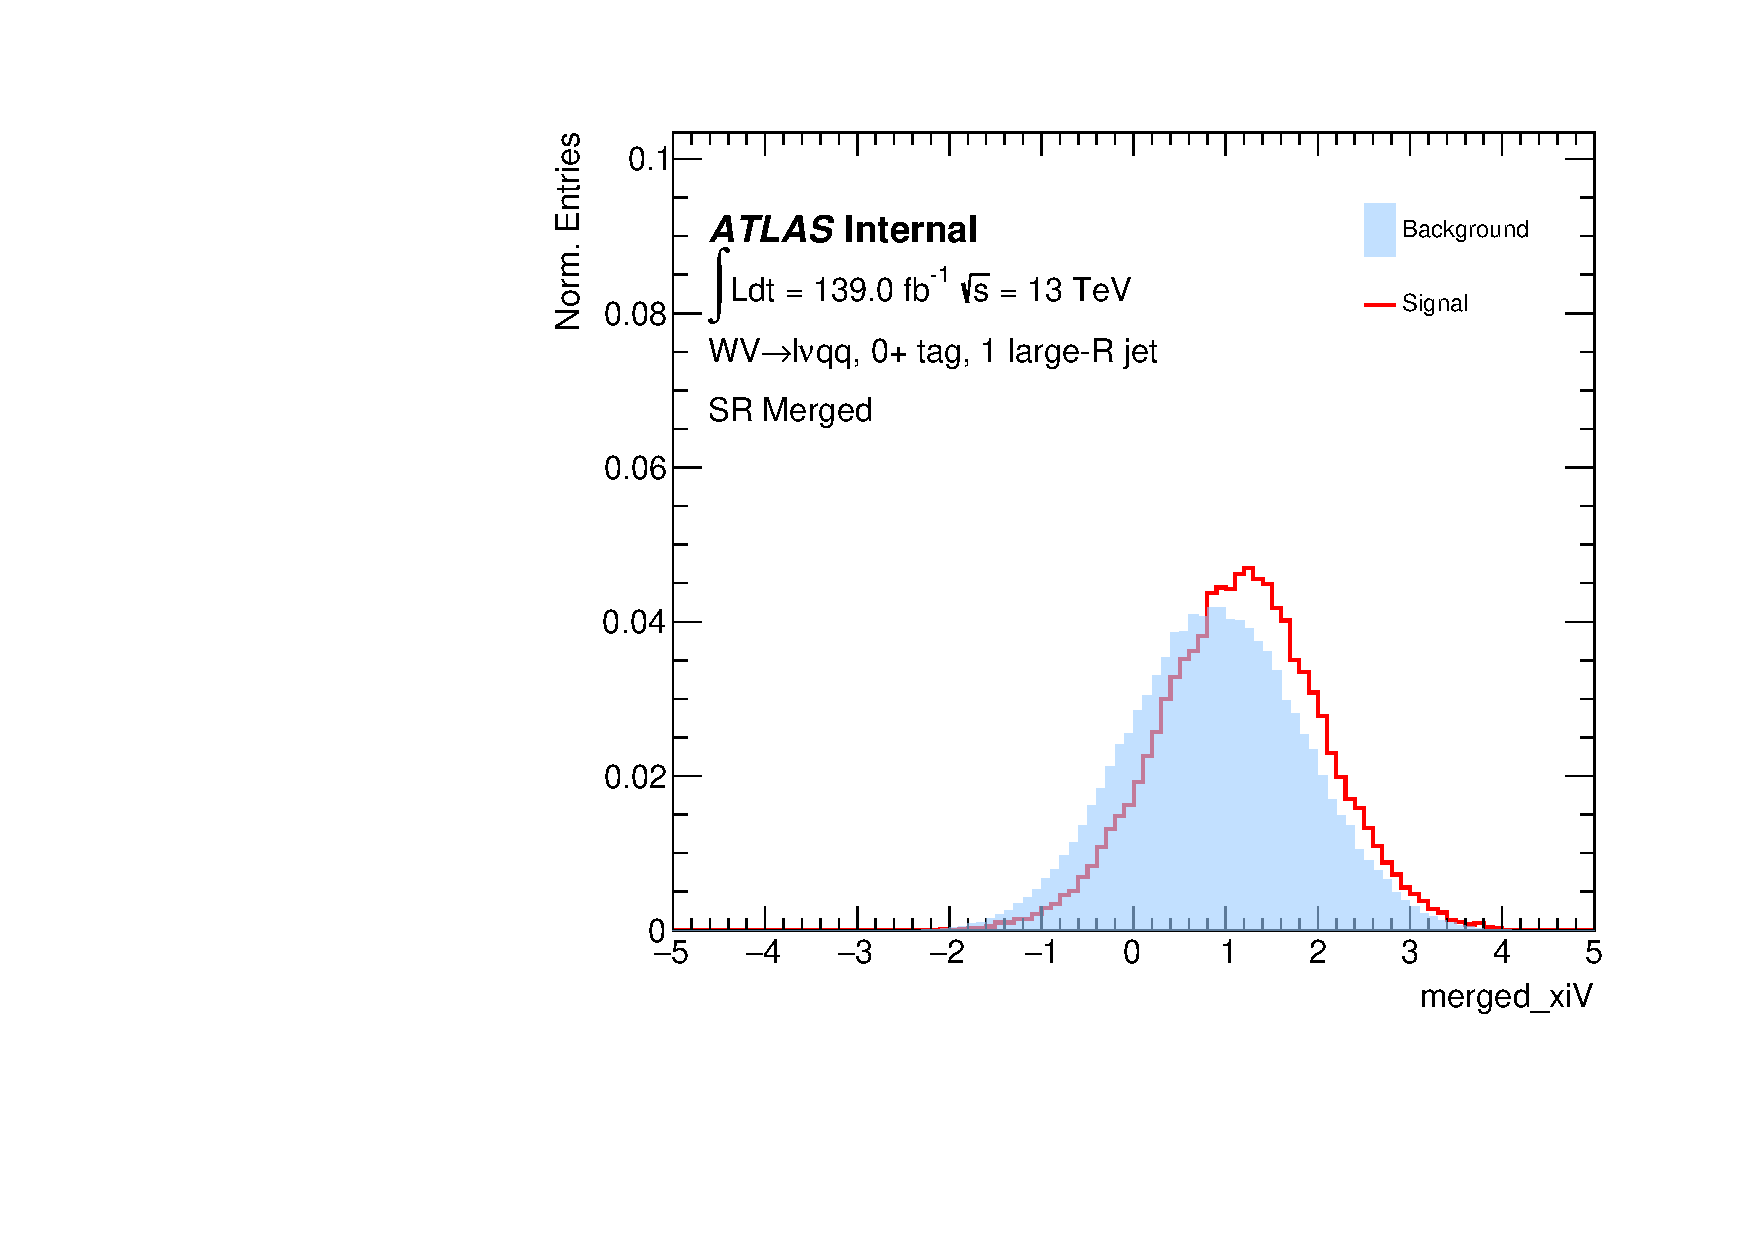
\includegraphics[width=0.3\textwidth]{figures/ml_dnn/variables/SR_Mer/norm_plot_merged_xiV.pdf}}\quad
  \subfloat[]{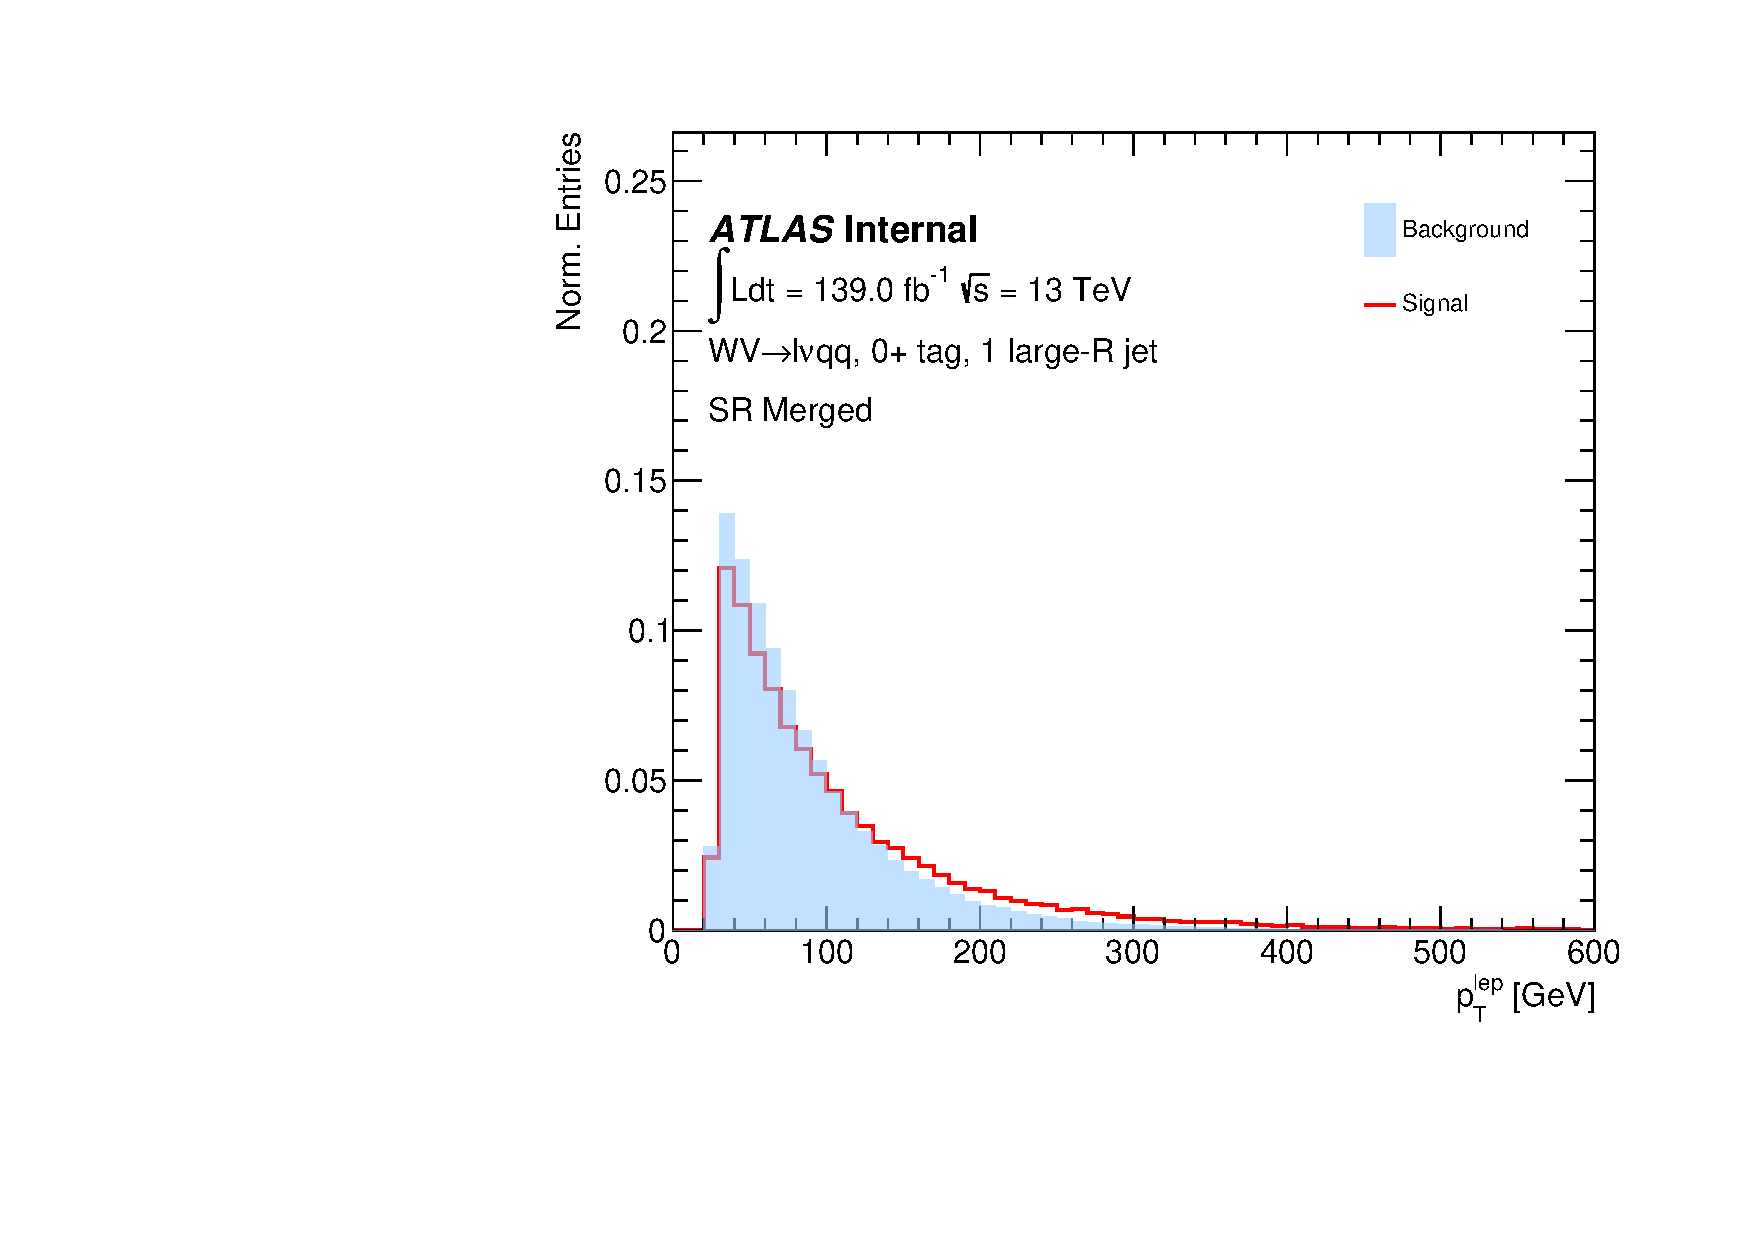
\includegraphics[width=0.3\textwidth]{figures/ml_dnn/variables/SR_Mer/norm_plot_lep_pt.pdf}}

  % Row 4
  \subfloat[]{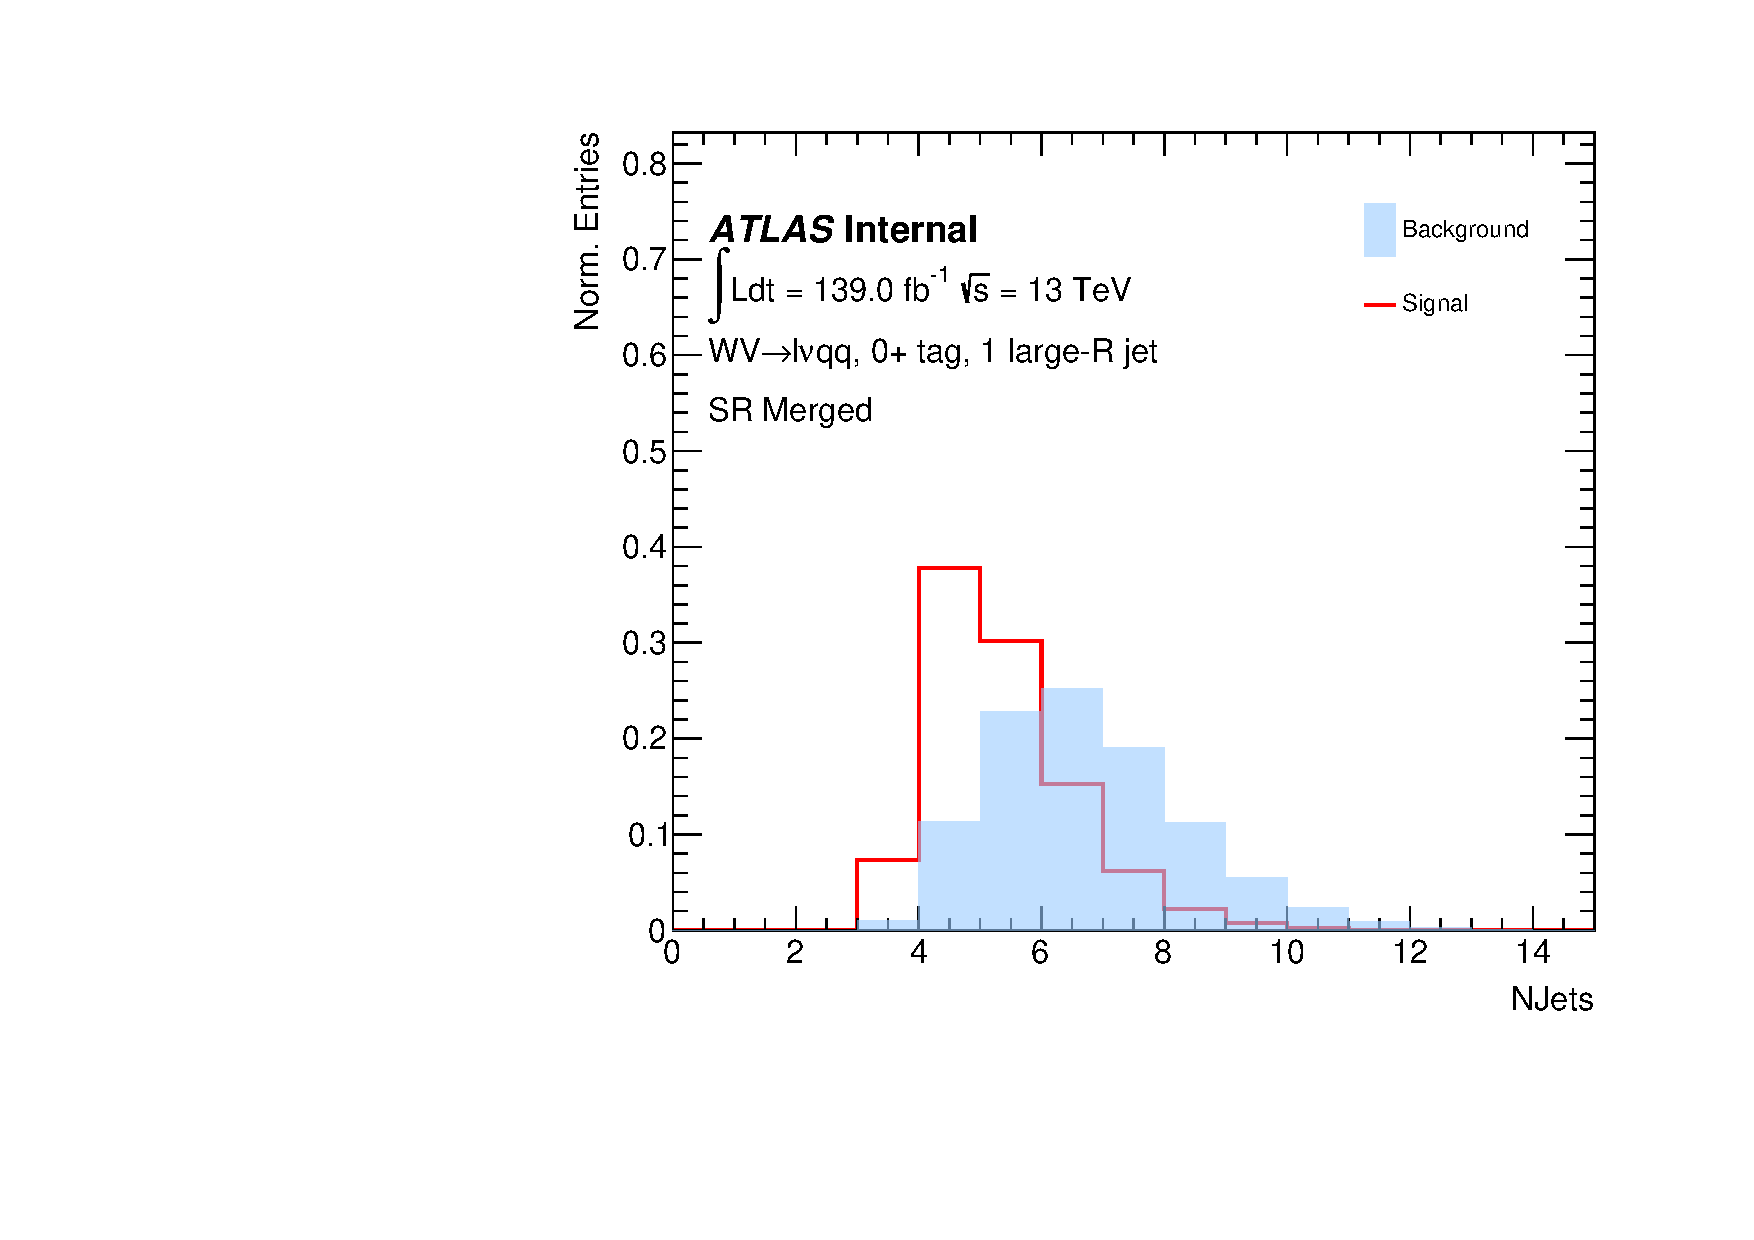
\includegraphics[width=0.3\textwidth]{figures/ml_dnn/variables/SR_Mer/norm_plot_NJets.pdf}}\quad
  \subfloat[]{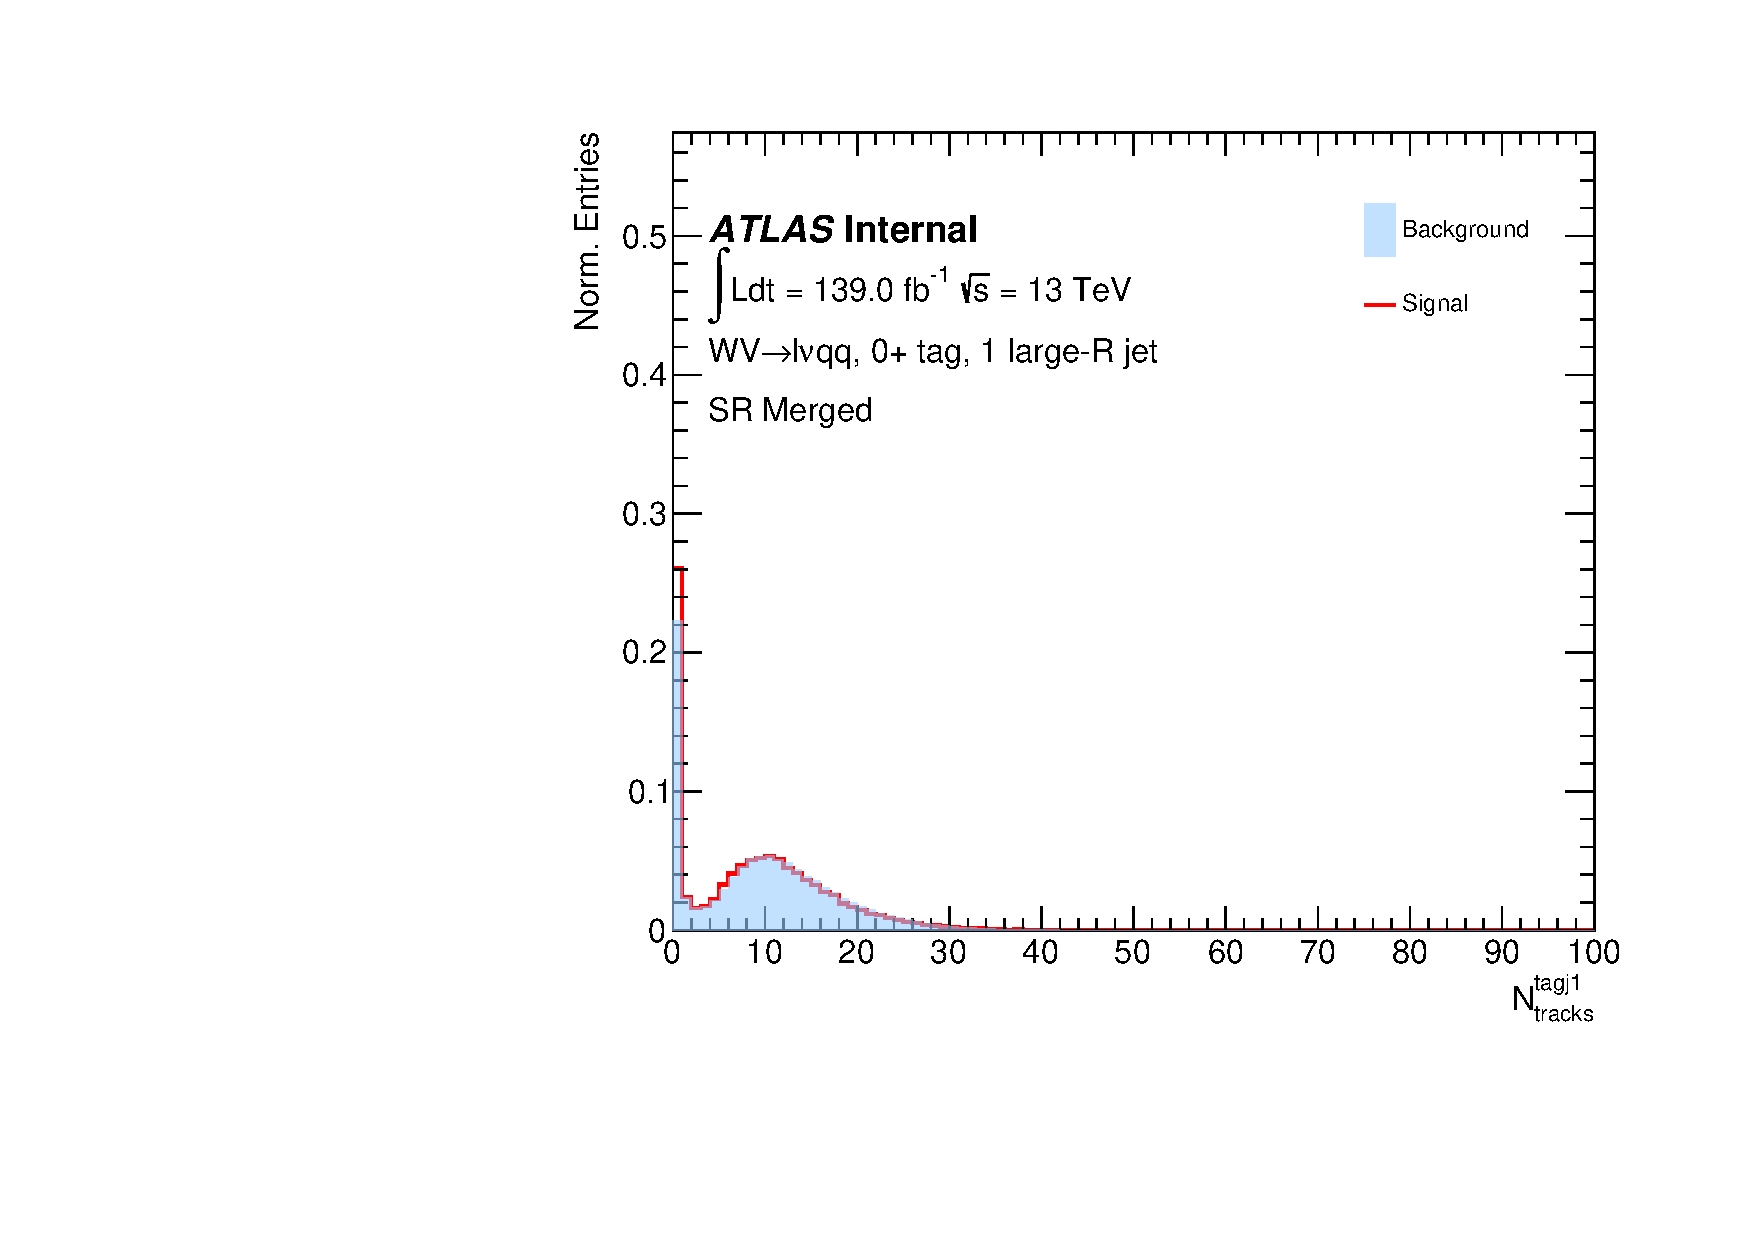
\includegraphics[width=0.3\textwidth]{figures/ml_dnn/variables/SR_Mer/norm_plot_merged_tagJ1_nTracks.pdf}}\quad
  \subfloat[]{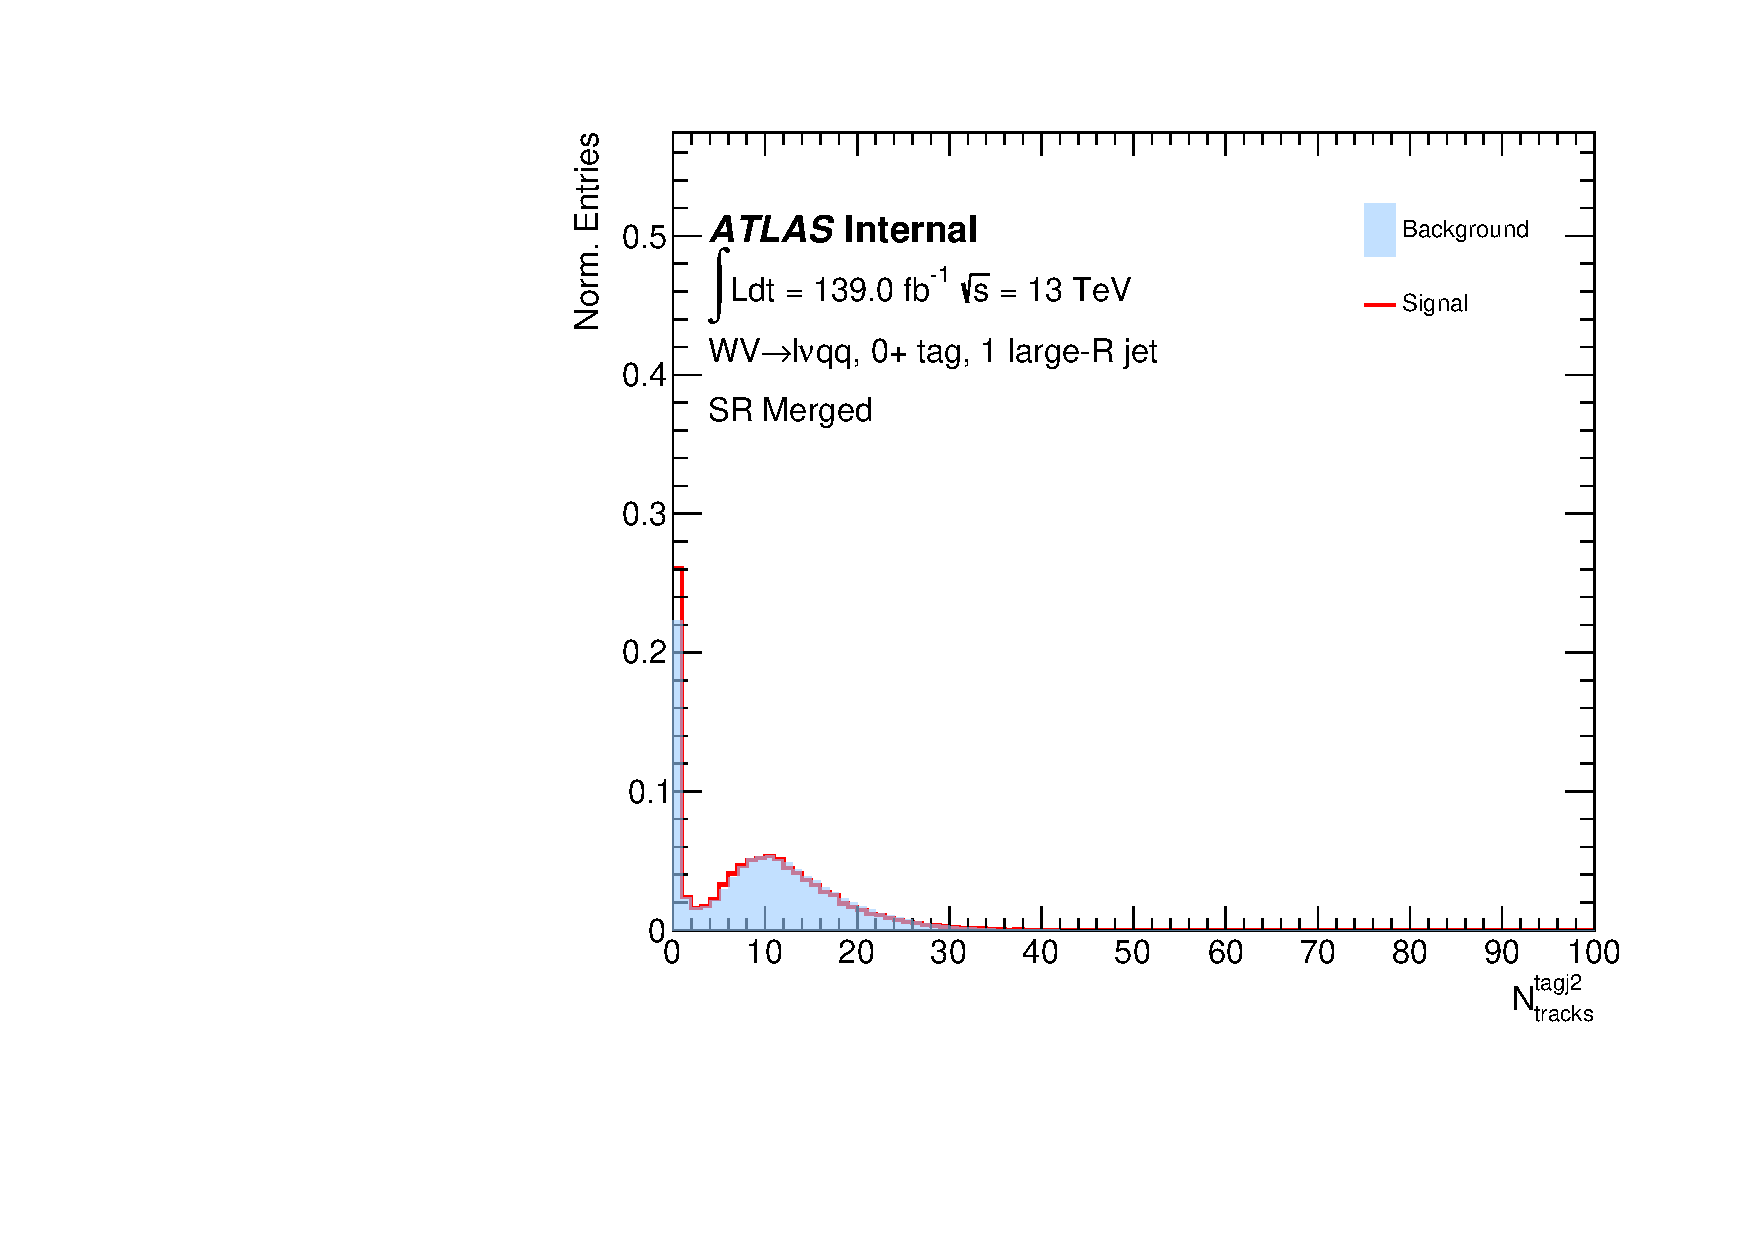
\includegraphics[width=0.3\textwidth]{figures/ml_dnn/variables/SR_Mer/norm_plot_merged_tagJ2_nTracks.pdf}}

  % Row 5
  \subfloat[]{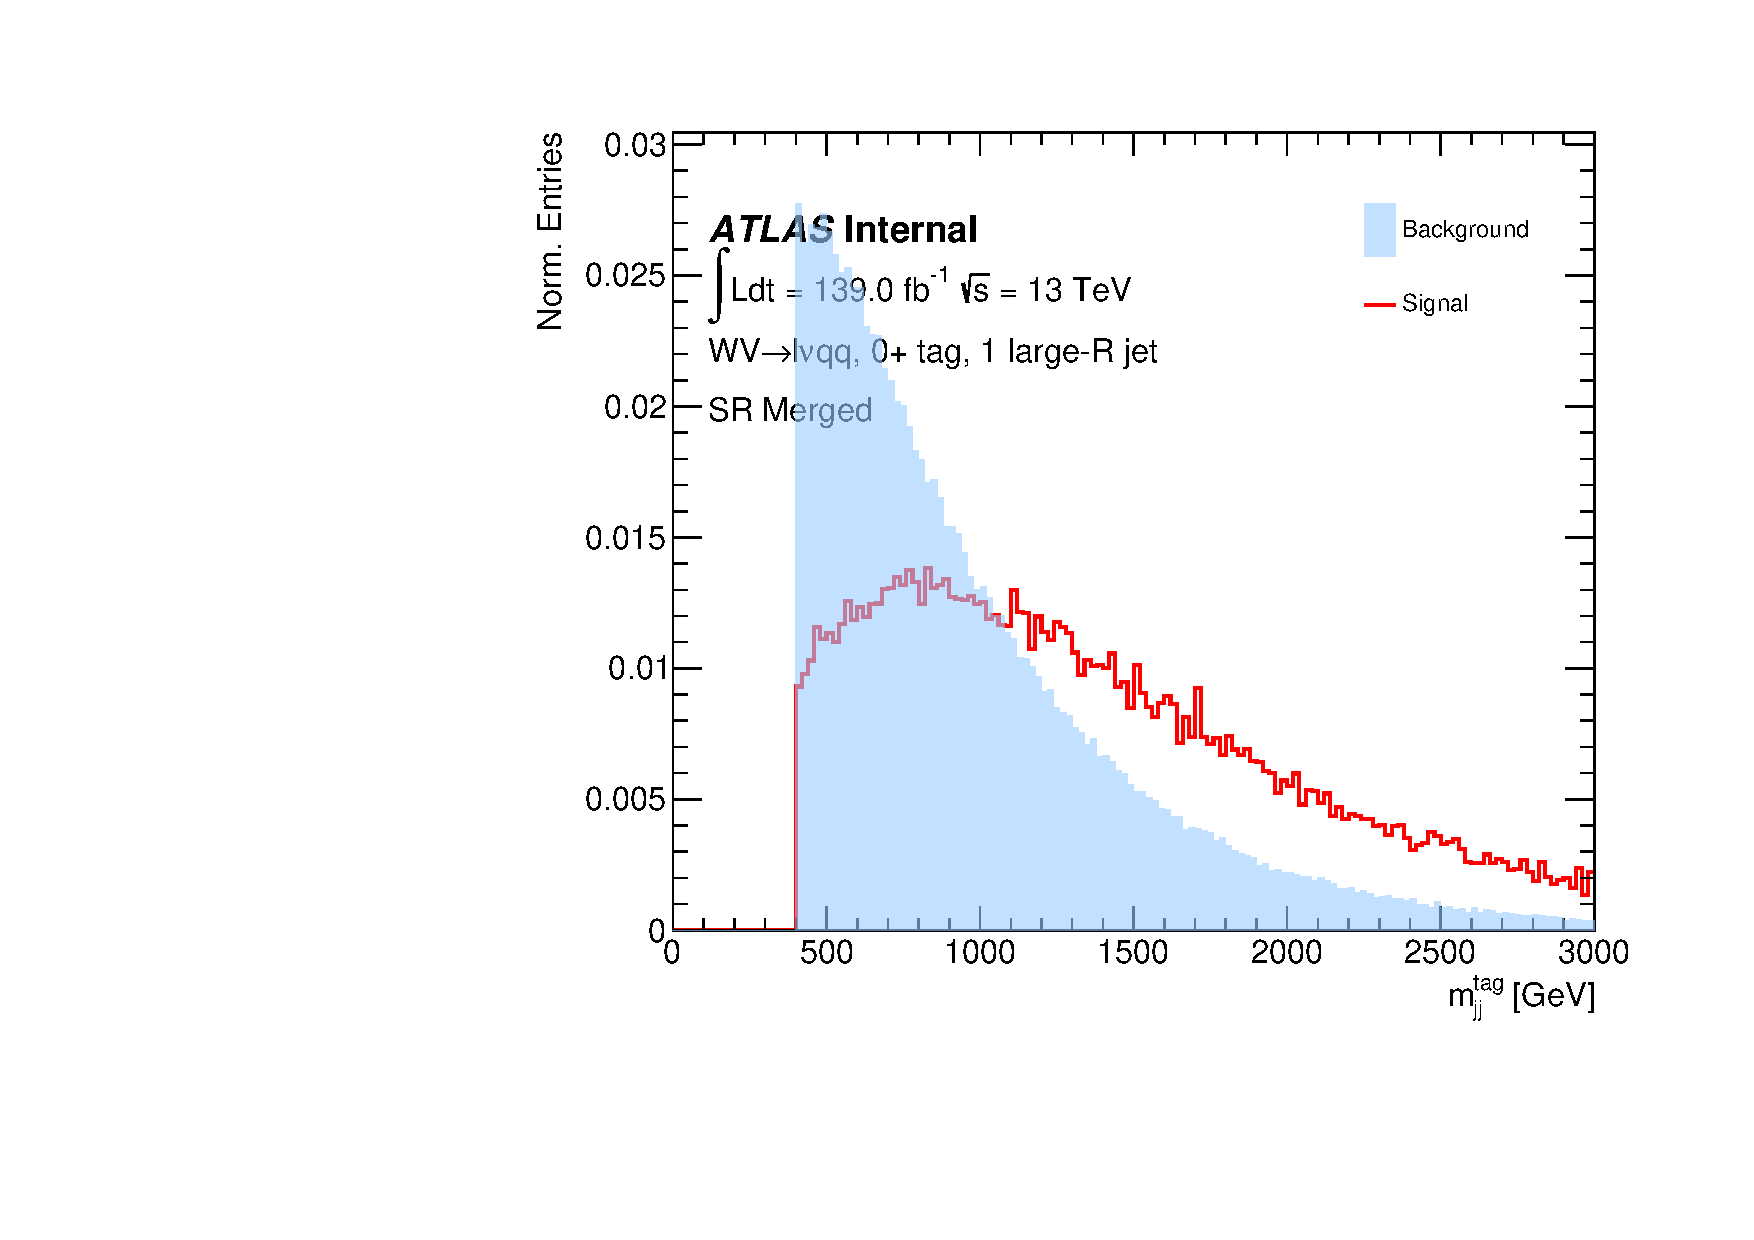
\includegraphics[width=0.3\textwidth]{figures/ml_dnn/variables/SR_Mer/norm_plot_merged_tagMjj.pdf}}\quad
  \subfloat[]{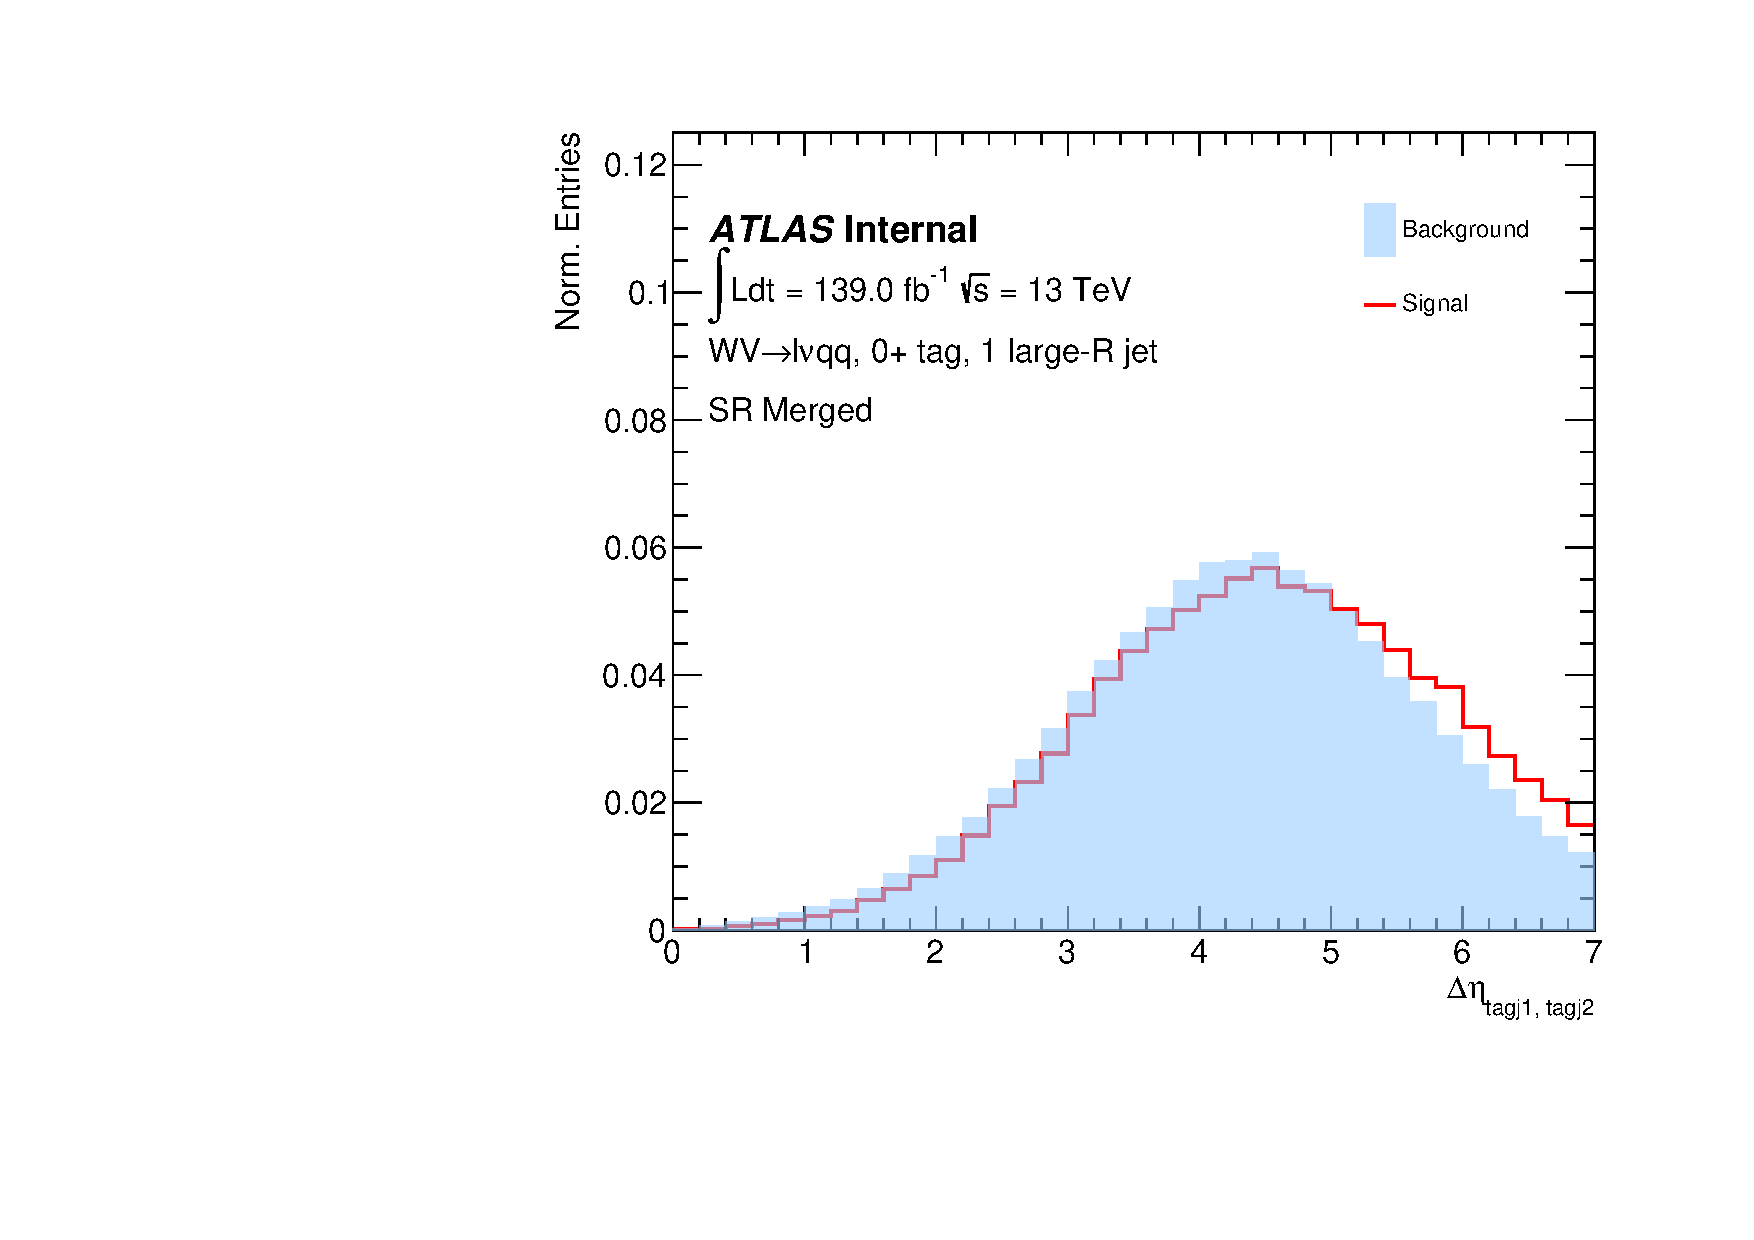
\includegraphics[width=0.3\textwidth]{figures/ml_dnn/variables/SR_Mer/norm_plot_merged_tagJdEta.pdf}}\quad
  \subfloat[]{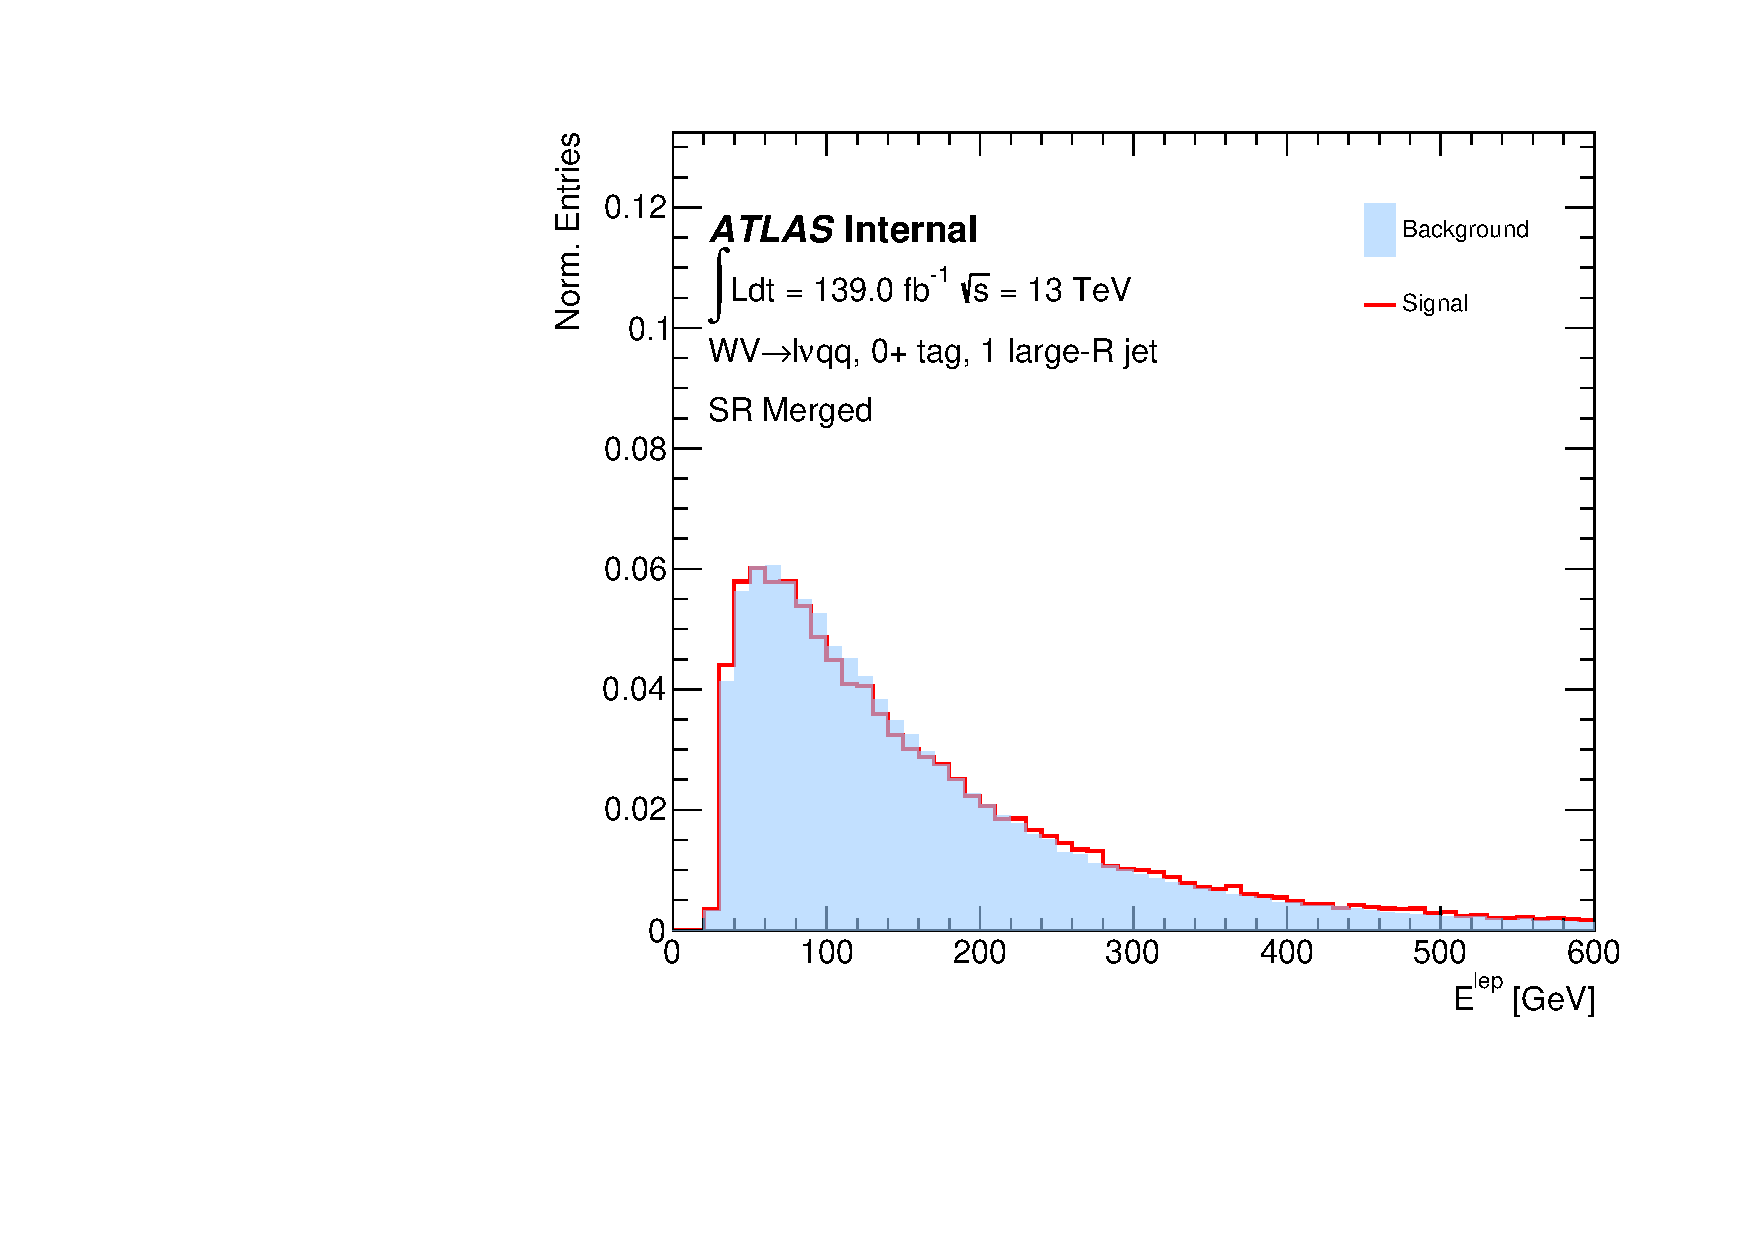
\includegraphics[width=0.3\textwidth]{figures/ml_dnn/variables/SR_Mer/norm_plot_lep_e.pdf}}

 \caption{Distributions of input variables in the Merged SR (Continued)}
 \label{fig:mer_inputs-part2}
\end{figure}

\begin{figure}[ht]
 \centering
  % Row 1
  \subfloat[]{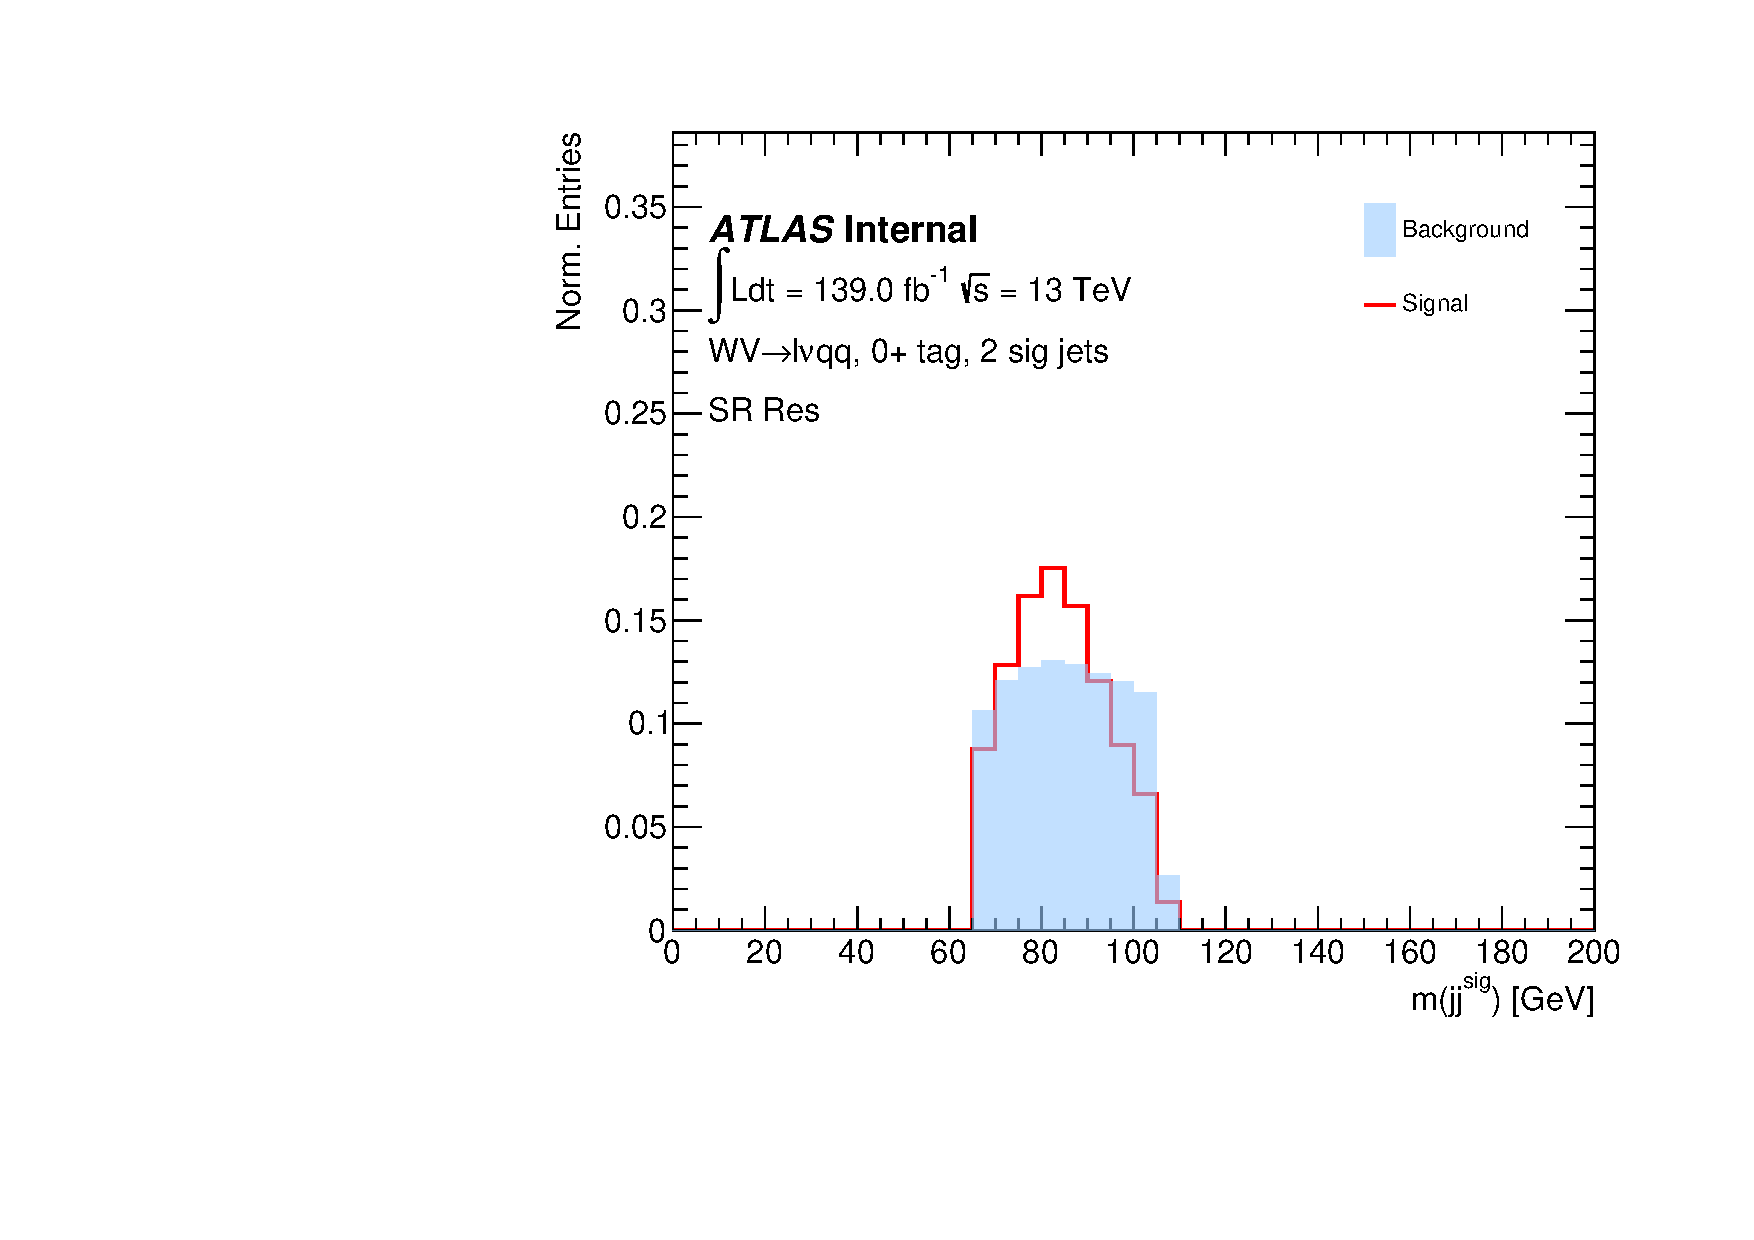
\includegraphics[width=0.3\textwidth]{figures/ml_dnn/variables/SR_Res/norm_plot_Dijet_m.pdf}}\quad
  \subfloat[]{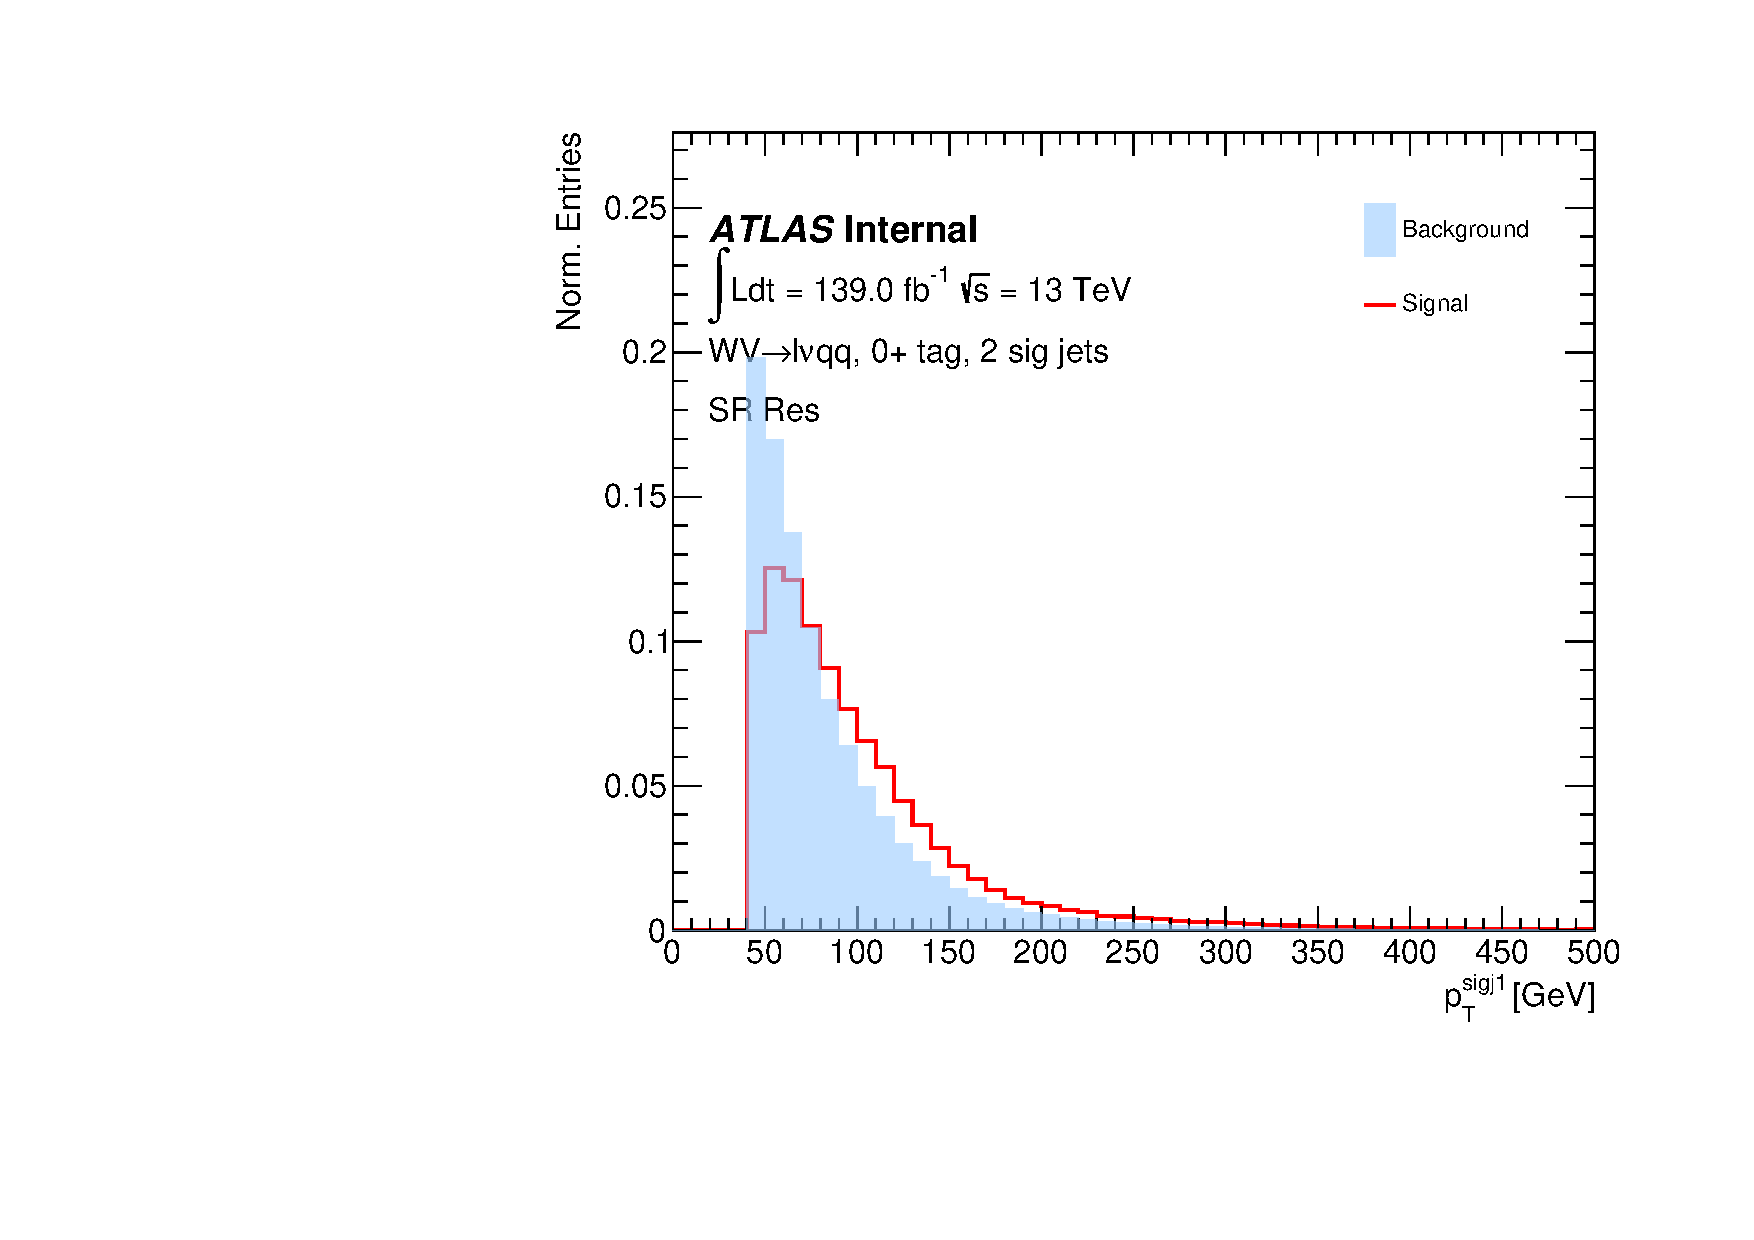
\includegraphics[width=0.3\textwidth]{figures/ml_dnn/variables/SR_Res/norm_plot_sigJ1_pt.pdf}}\quad
  \subfloat[]{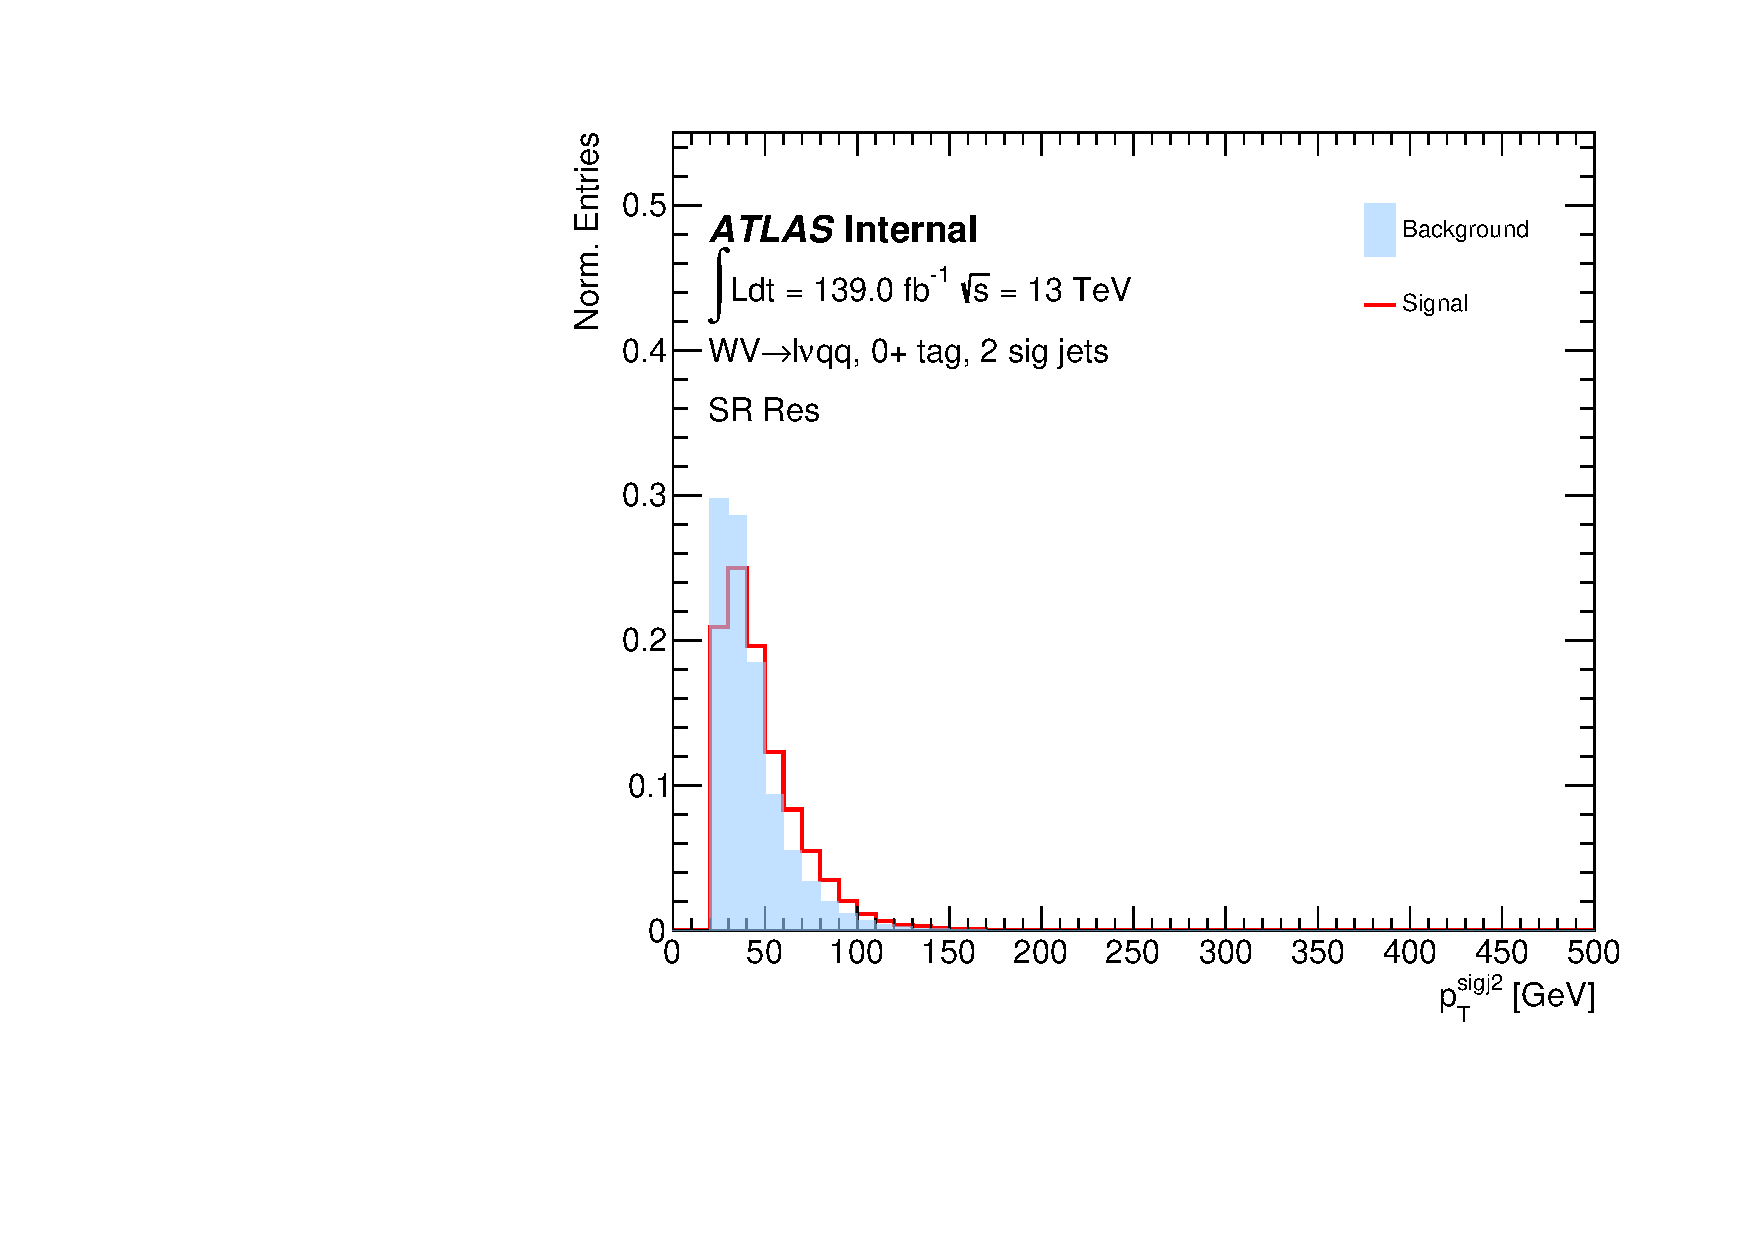
\includegraphics[width=0.3\textwidth]{figures/ml_dnn/variables/SR_Res/norm_plot_sigJ2_pt.pdf}}
  
  % Row 2
  \subfloat[]{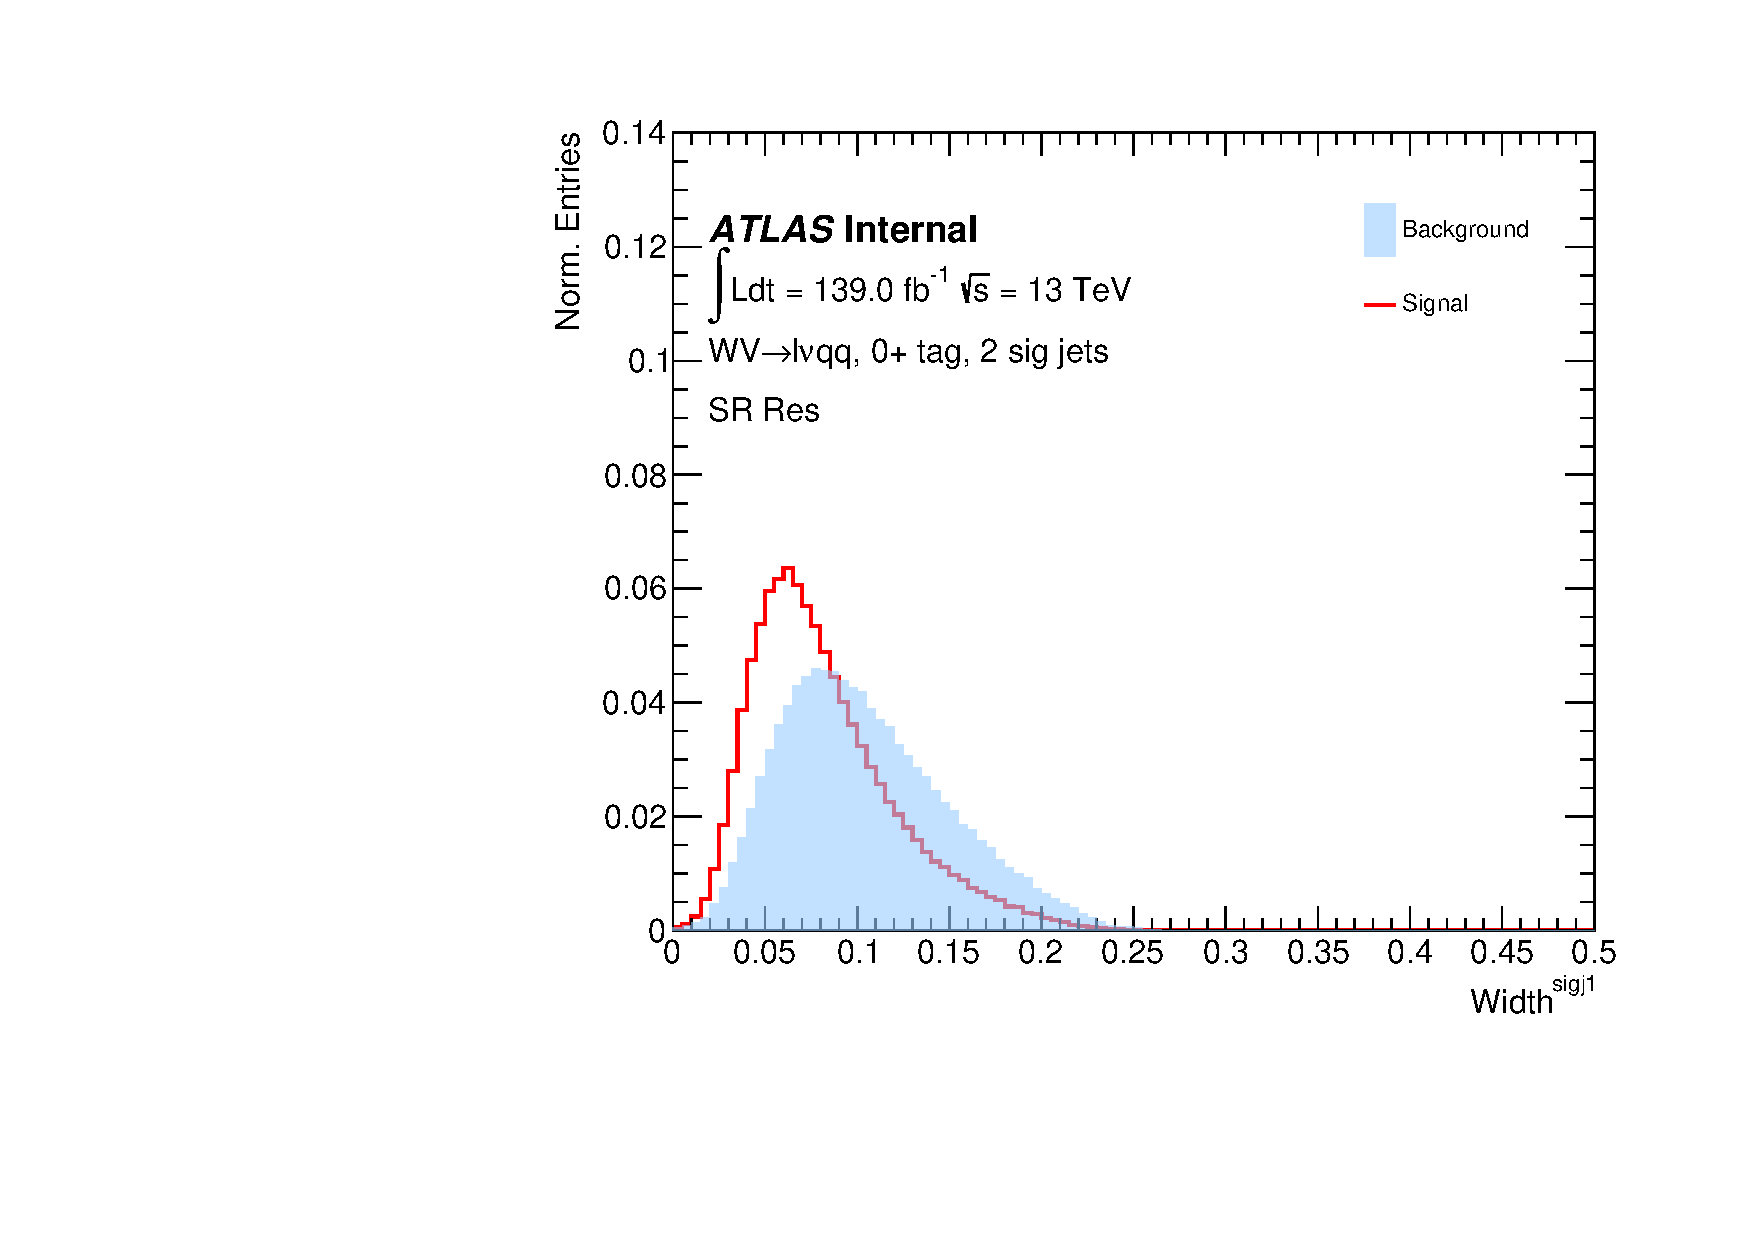
\includegraphics[width=0.3\textwidth]{figures/ml_dnn/variables/SR_Res/norm_plot_sigJ1_width.pdf}}\quad
  \subfloat[]{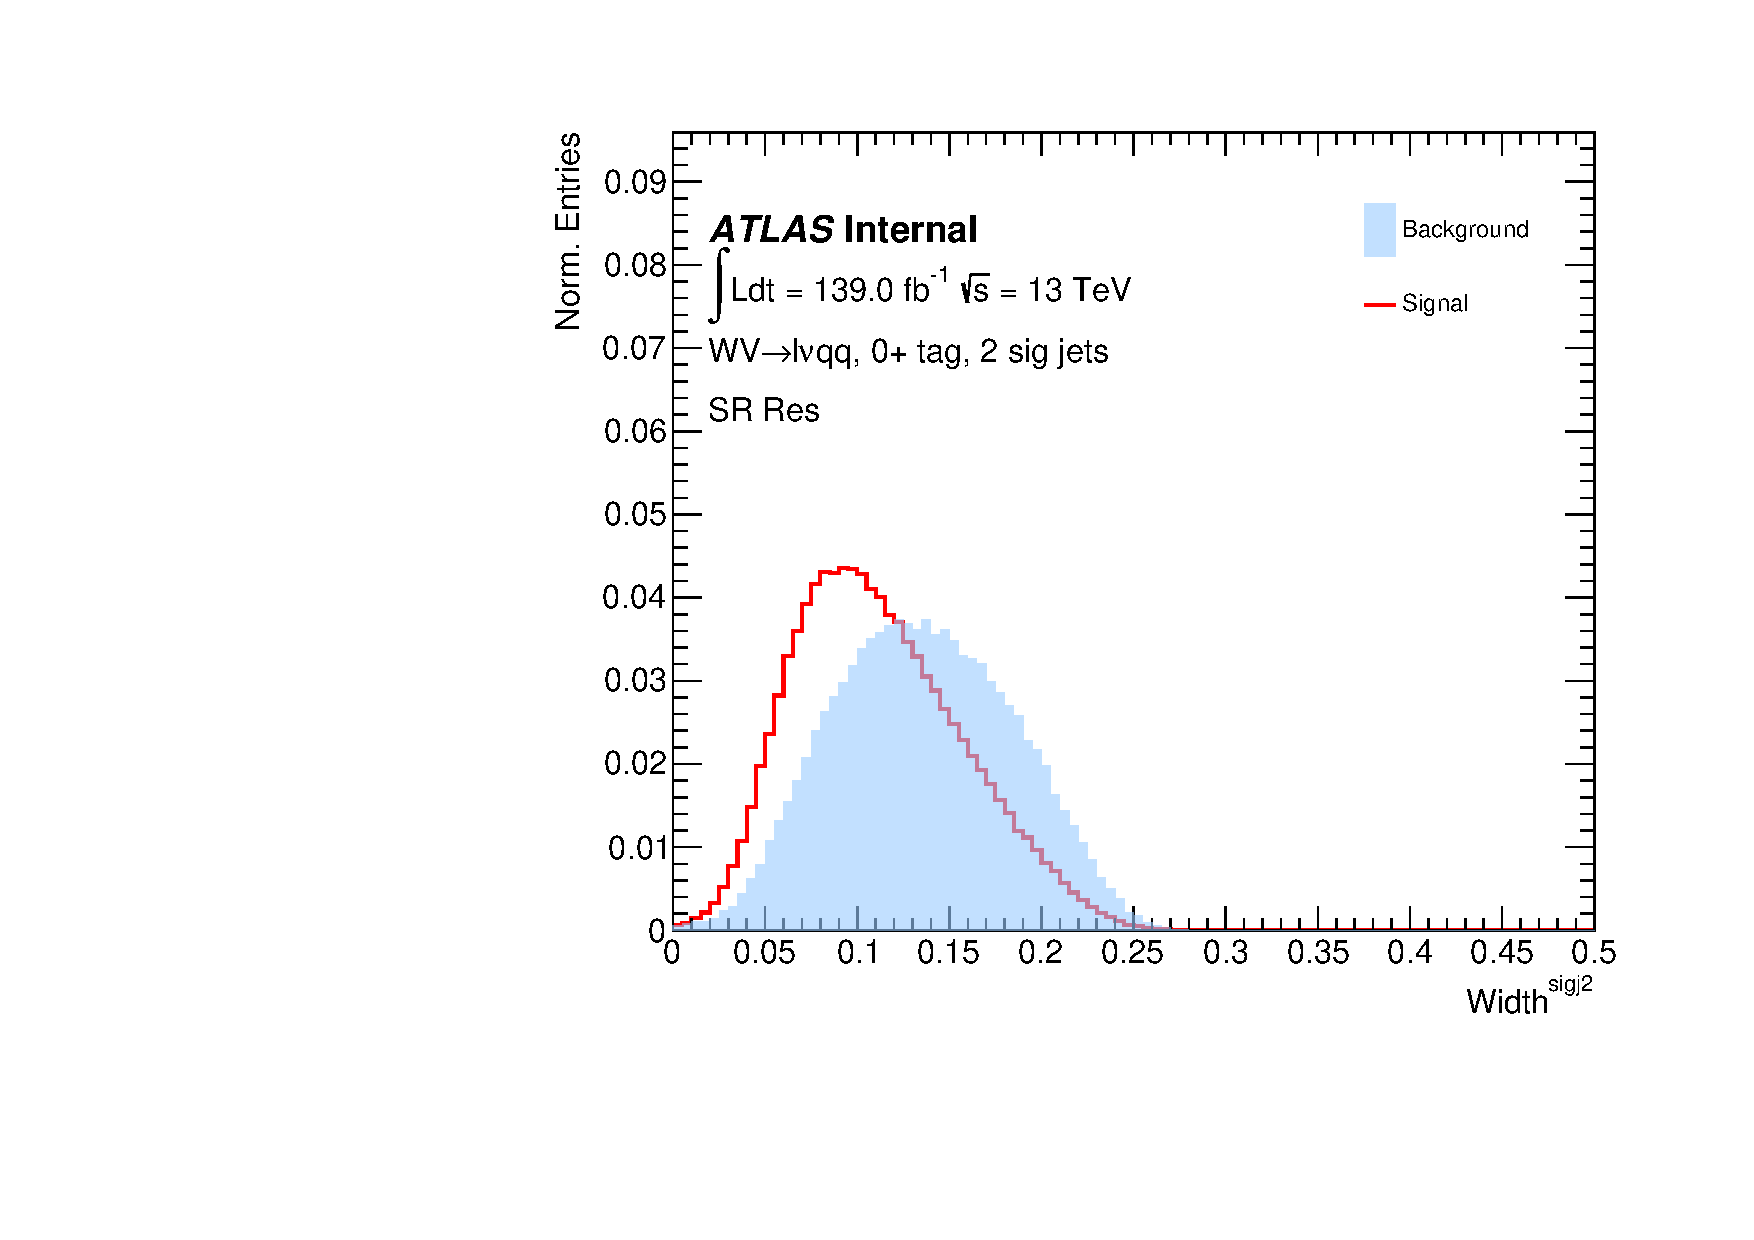
\includegraphics[width=0.3\textwidth]{figures/ml_dnn/variables/SR_Res/norm_plot_sigJ2_width.pdf}}\quad
  \subfloat[]{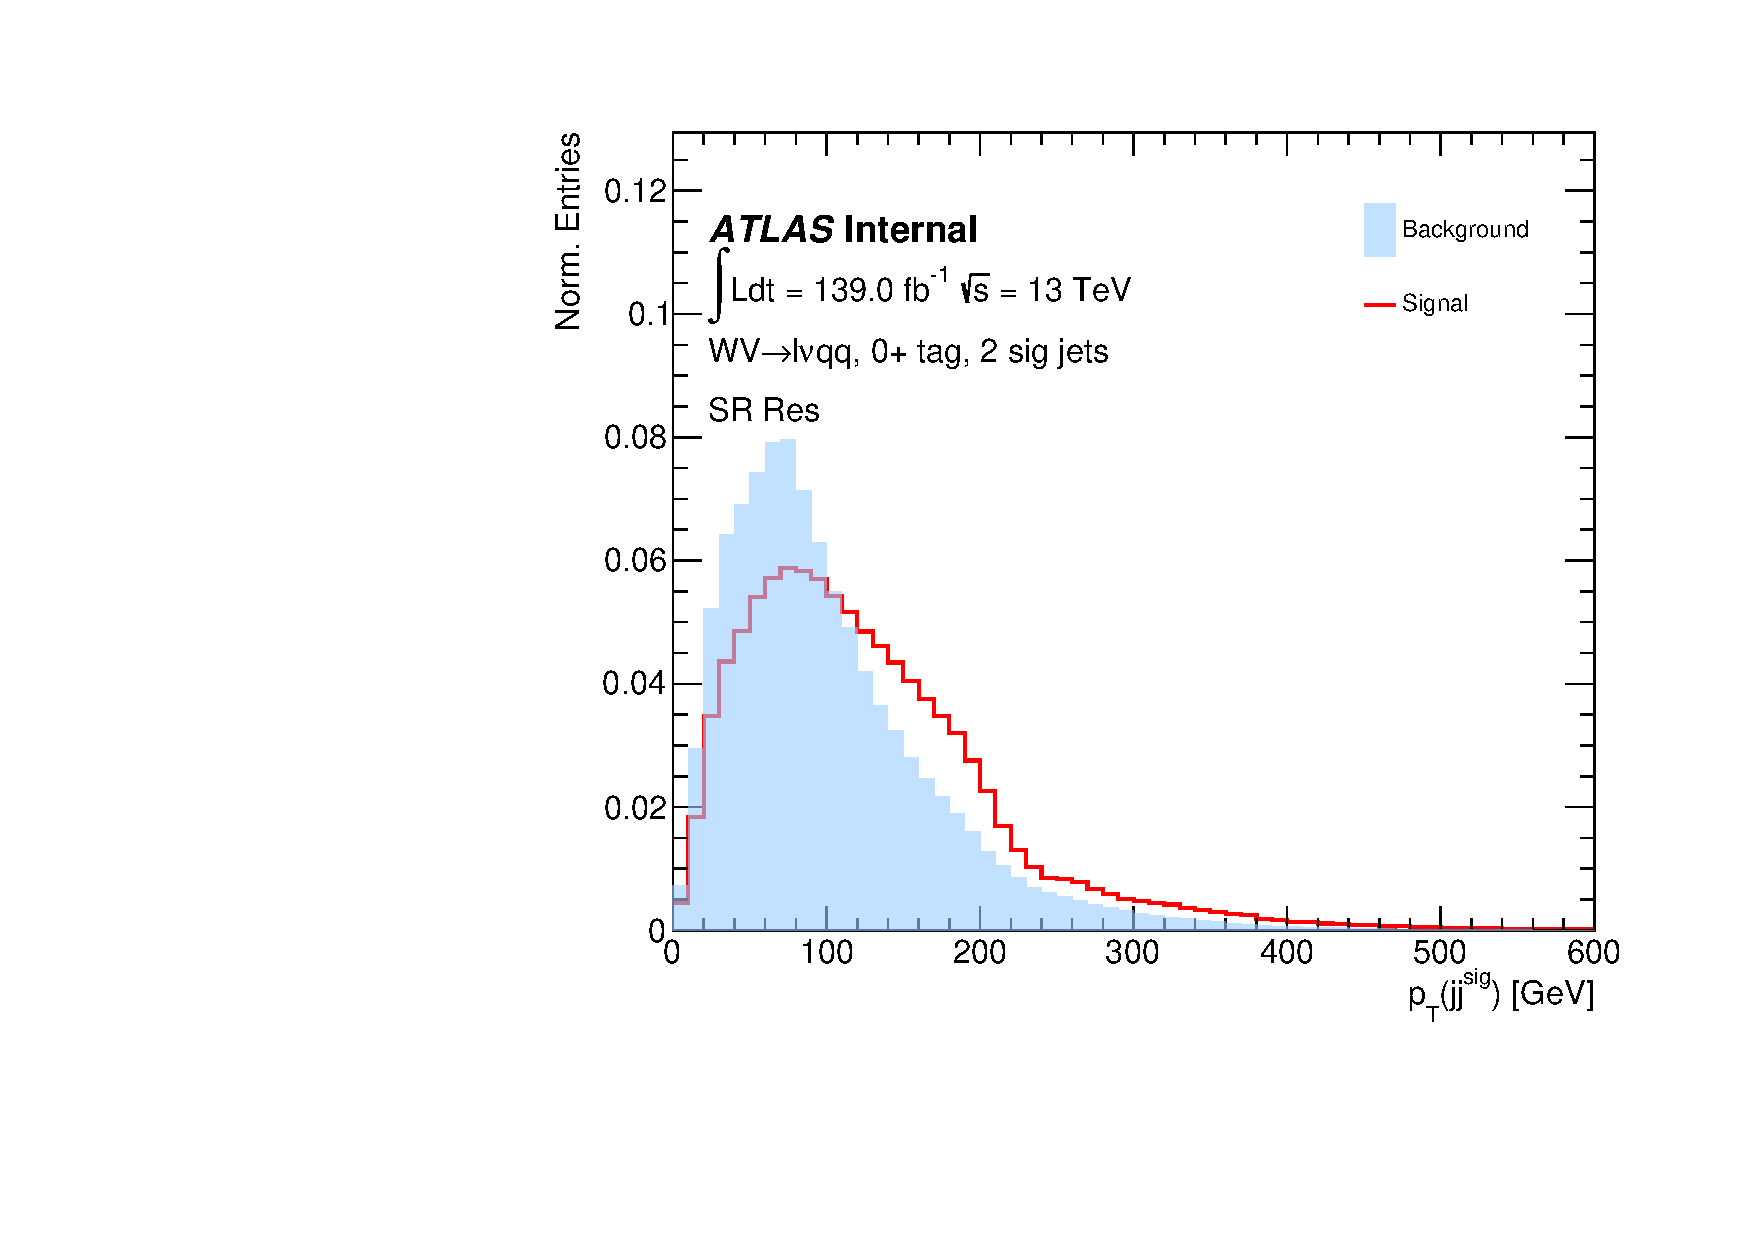
\includegraphics[width=0.3\textwidth]{figures/ml_dnn/variables/SR_Res/norm_plot_Dijet_pt.pdf}}
  
  % Row 3
  \subfloat[]{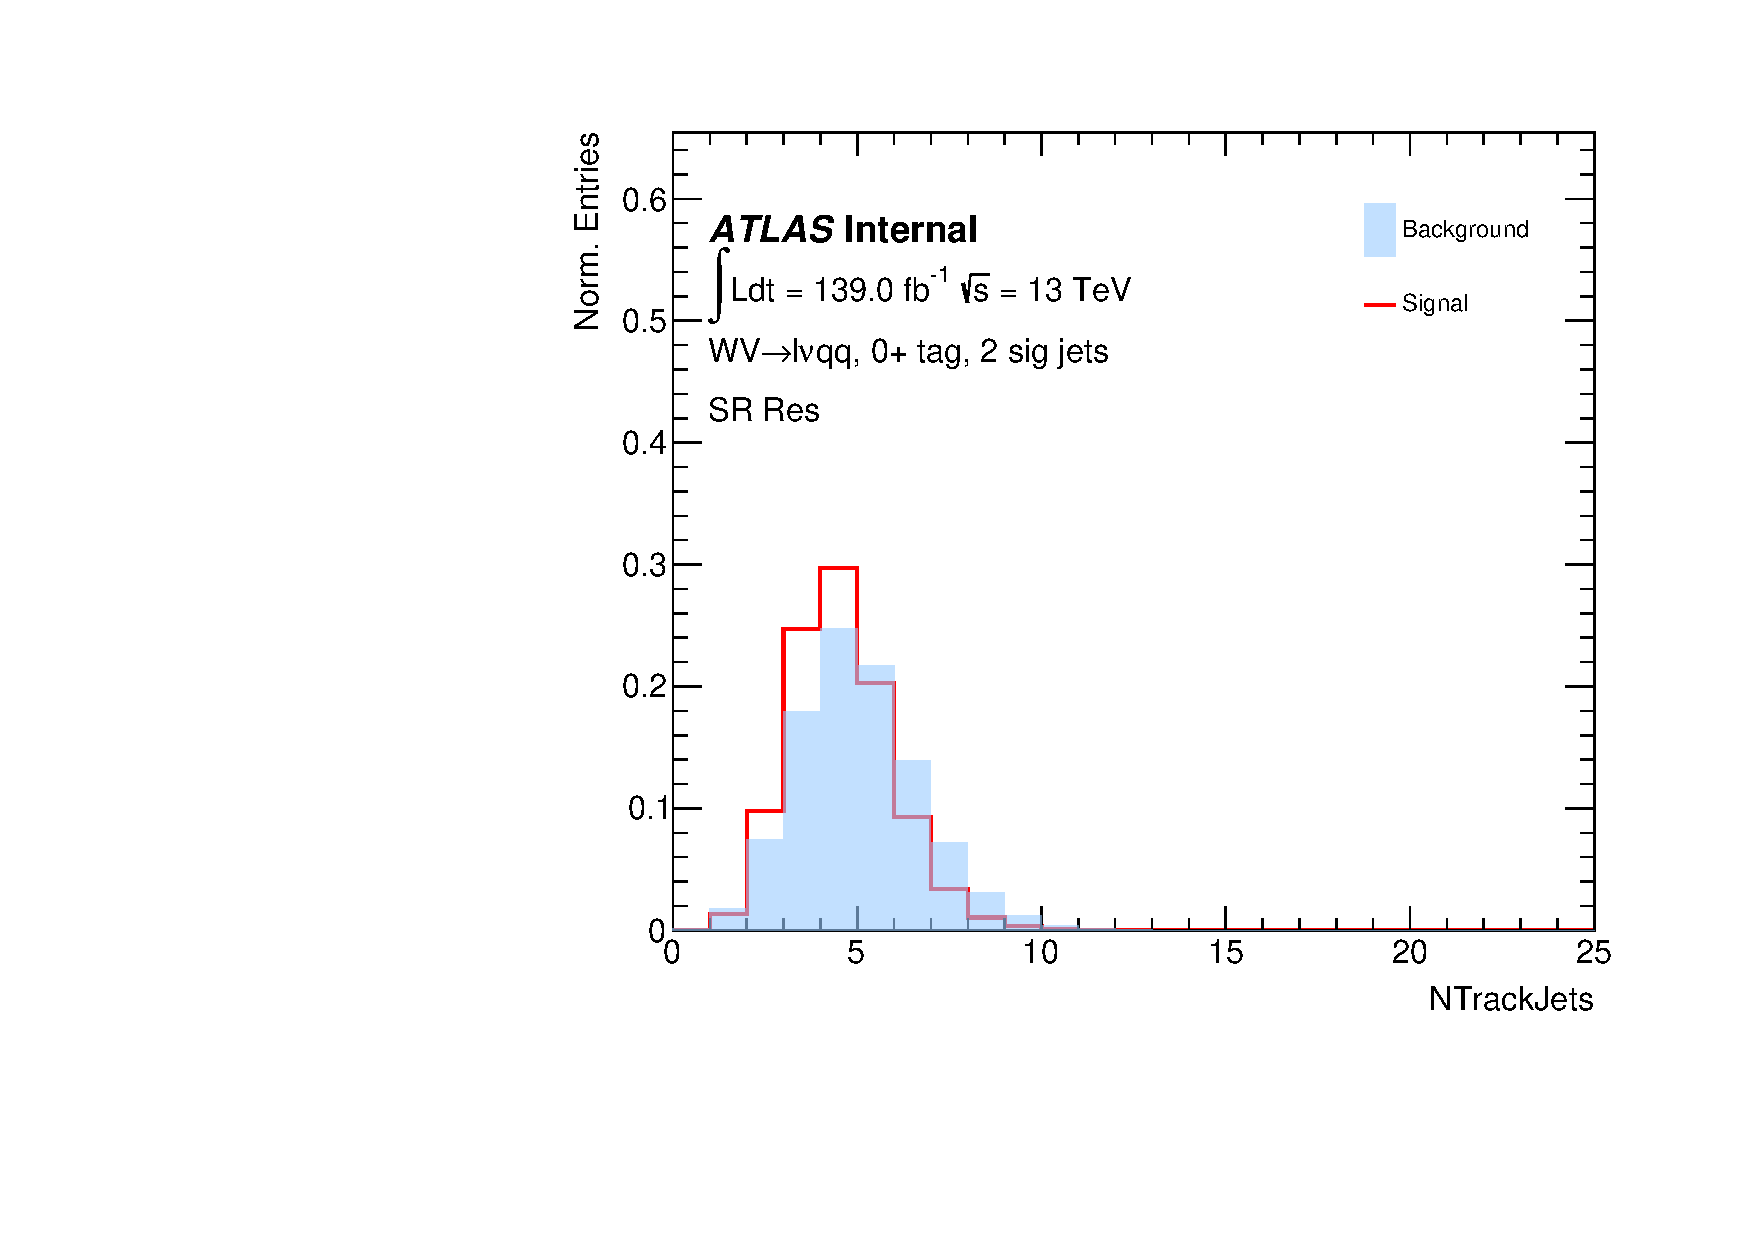
\includegraphics[width=0.3\textwidth]{figures/ml_dnn/variables/SR_Res/norm_plot_NTrackJets.pdf}}\quad
  \subfloat[]{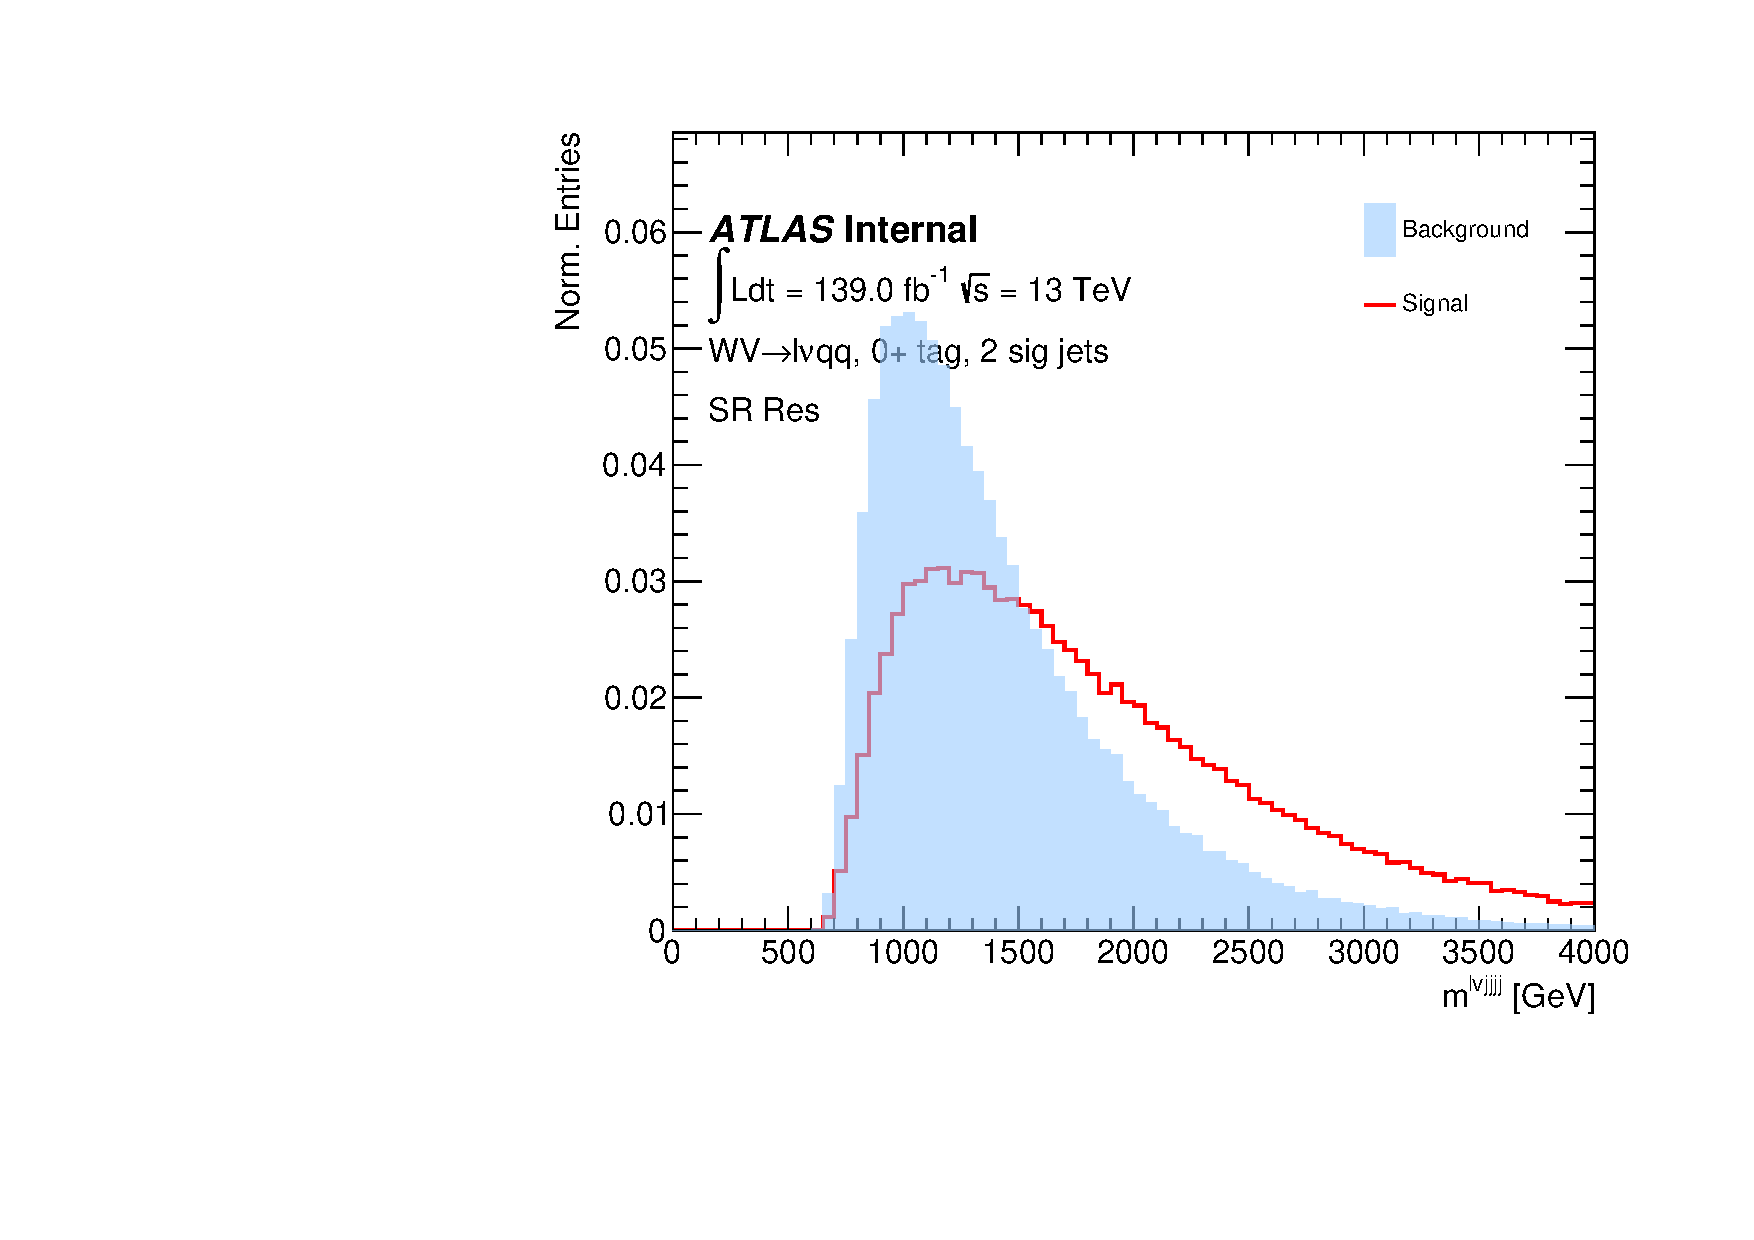
\includegraphics[width=0.3\textwidth]{figures/ml_dnn/variables/SR_Res/norm_plot_lvjjjjmass.pdf}}\quad
  \subfloat[]{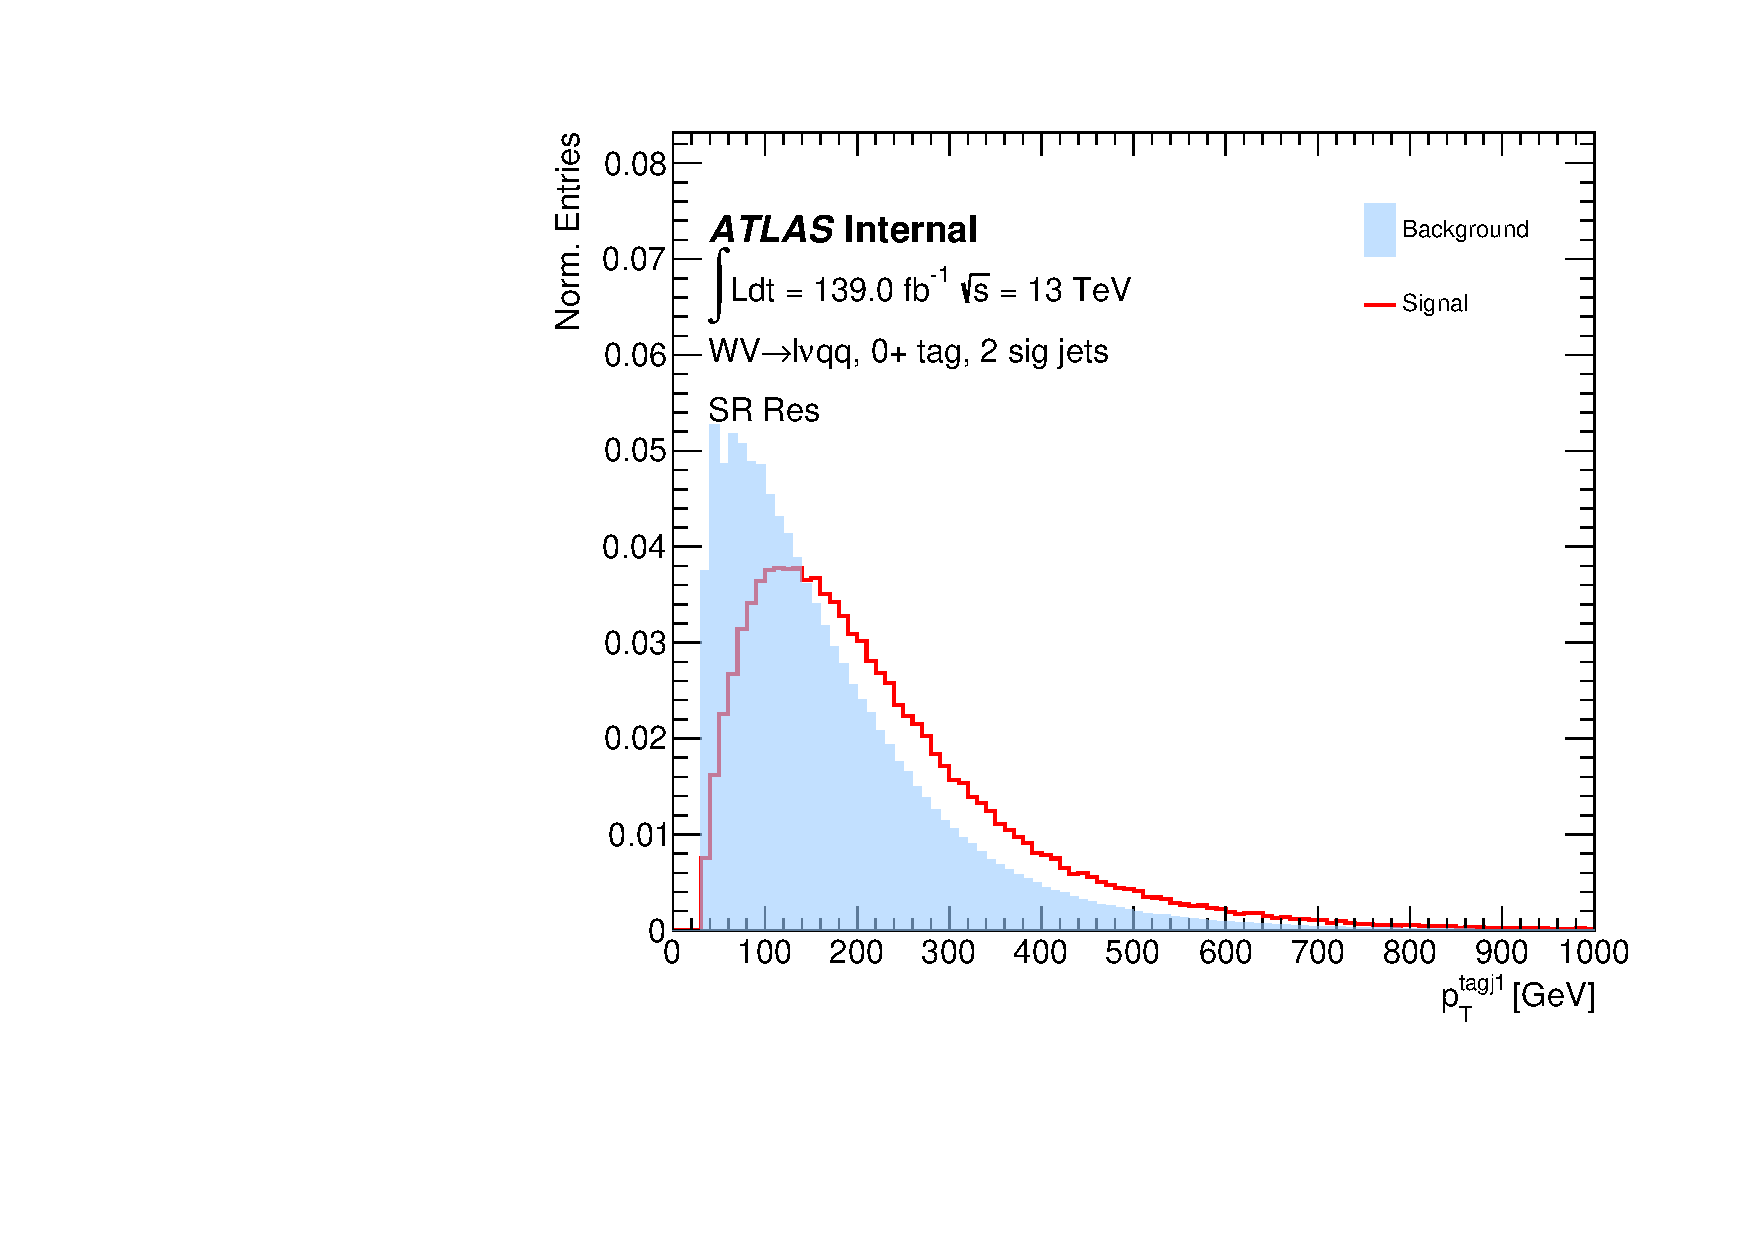
\includegraphics[width=0.3\textwidth]{figures/ml_dnn/variables/SR_Res/norm_plot_resolved_tagJ1_pt.pdf}}
  
 \caption{Distributions of input variables in the Resolved SR (Continued on next page)}
 \label{fig:res_inputs-part1}
\end{figure}

\begin{figure}[ht]
 \centering

  % Row 4
  \subfloat[]{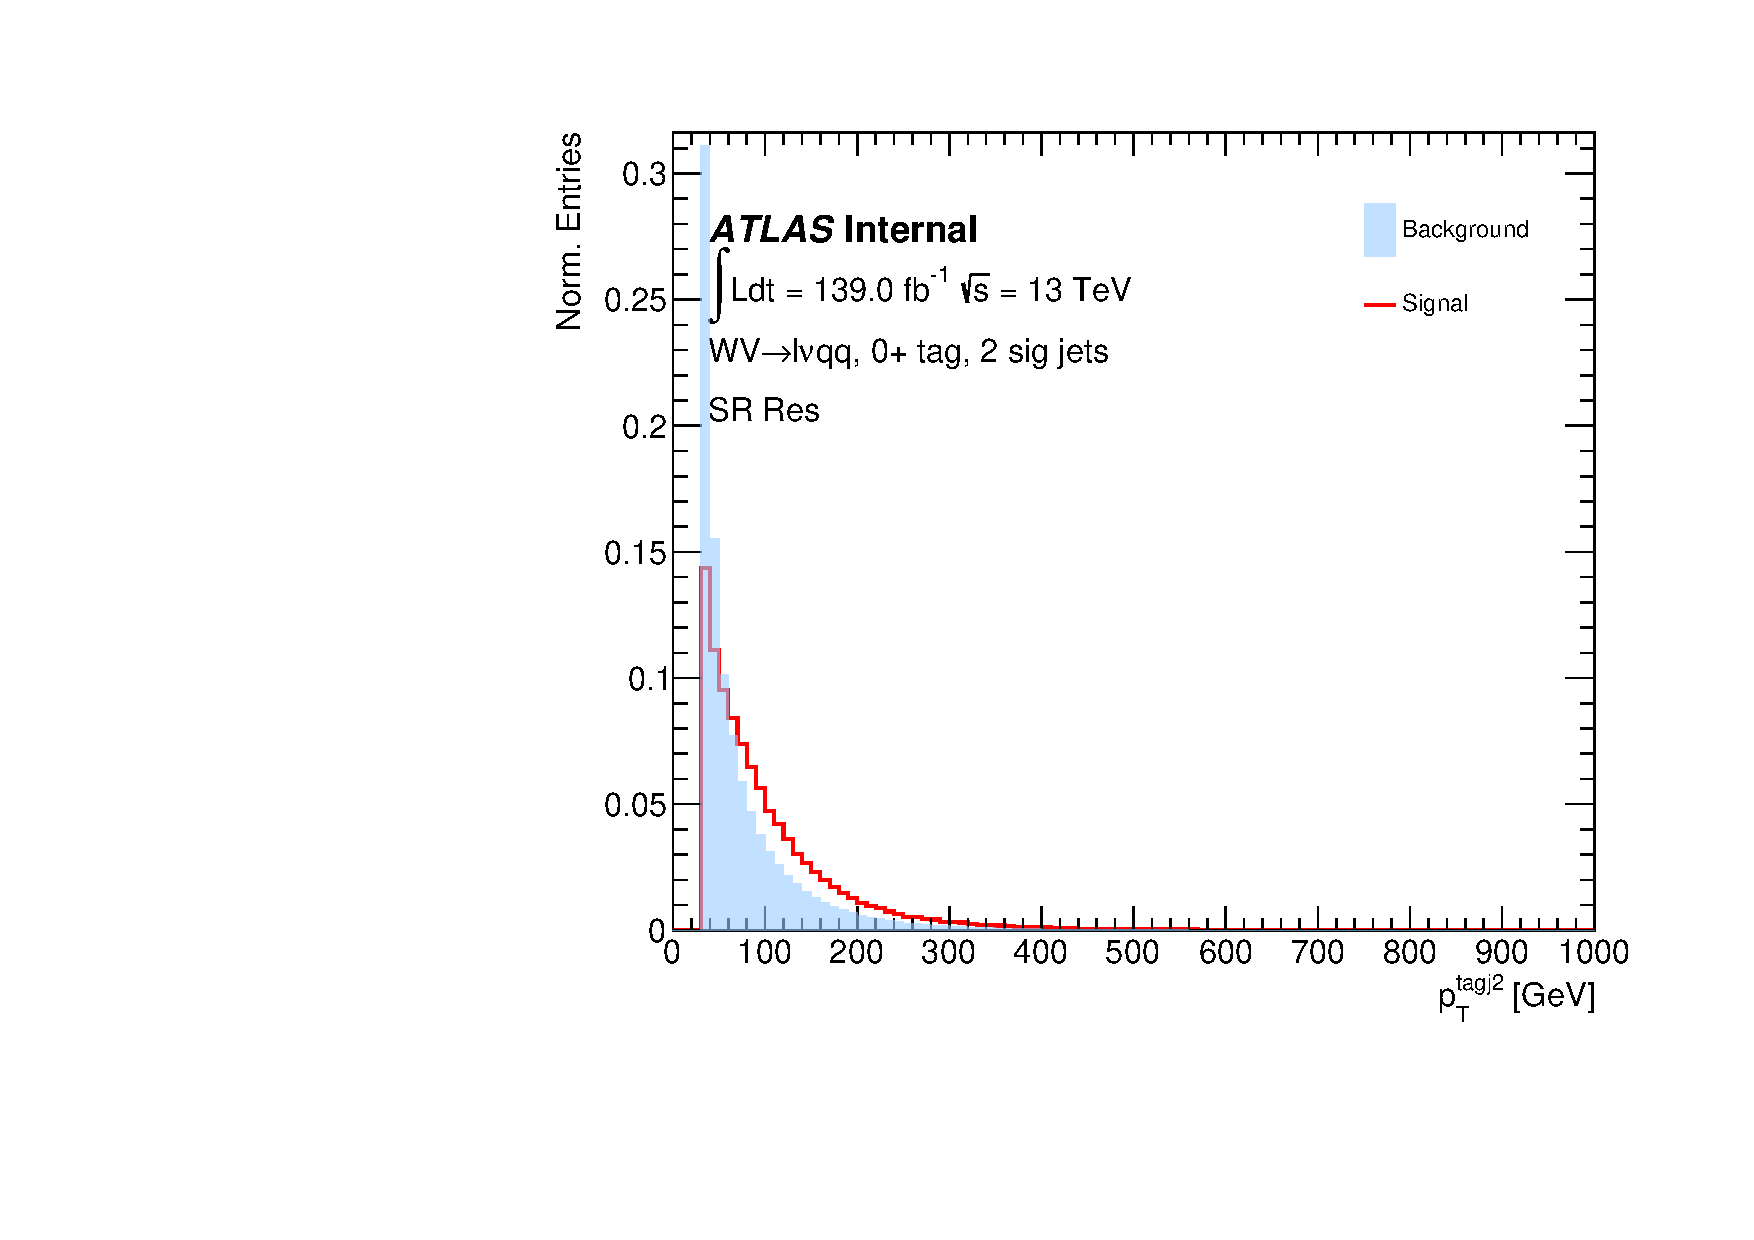
\includegraphics[width=0.3\textwidth]{figures/ml_dnn/variables/SR_Res/norm_plot_resolved_tagJ2_pt.pdf}}\quad
  \subfloat[]{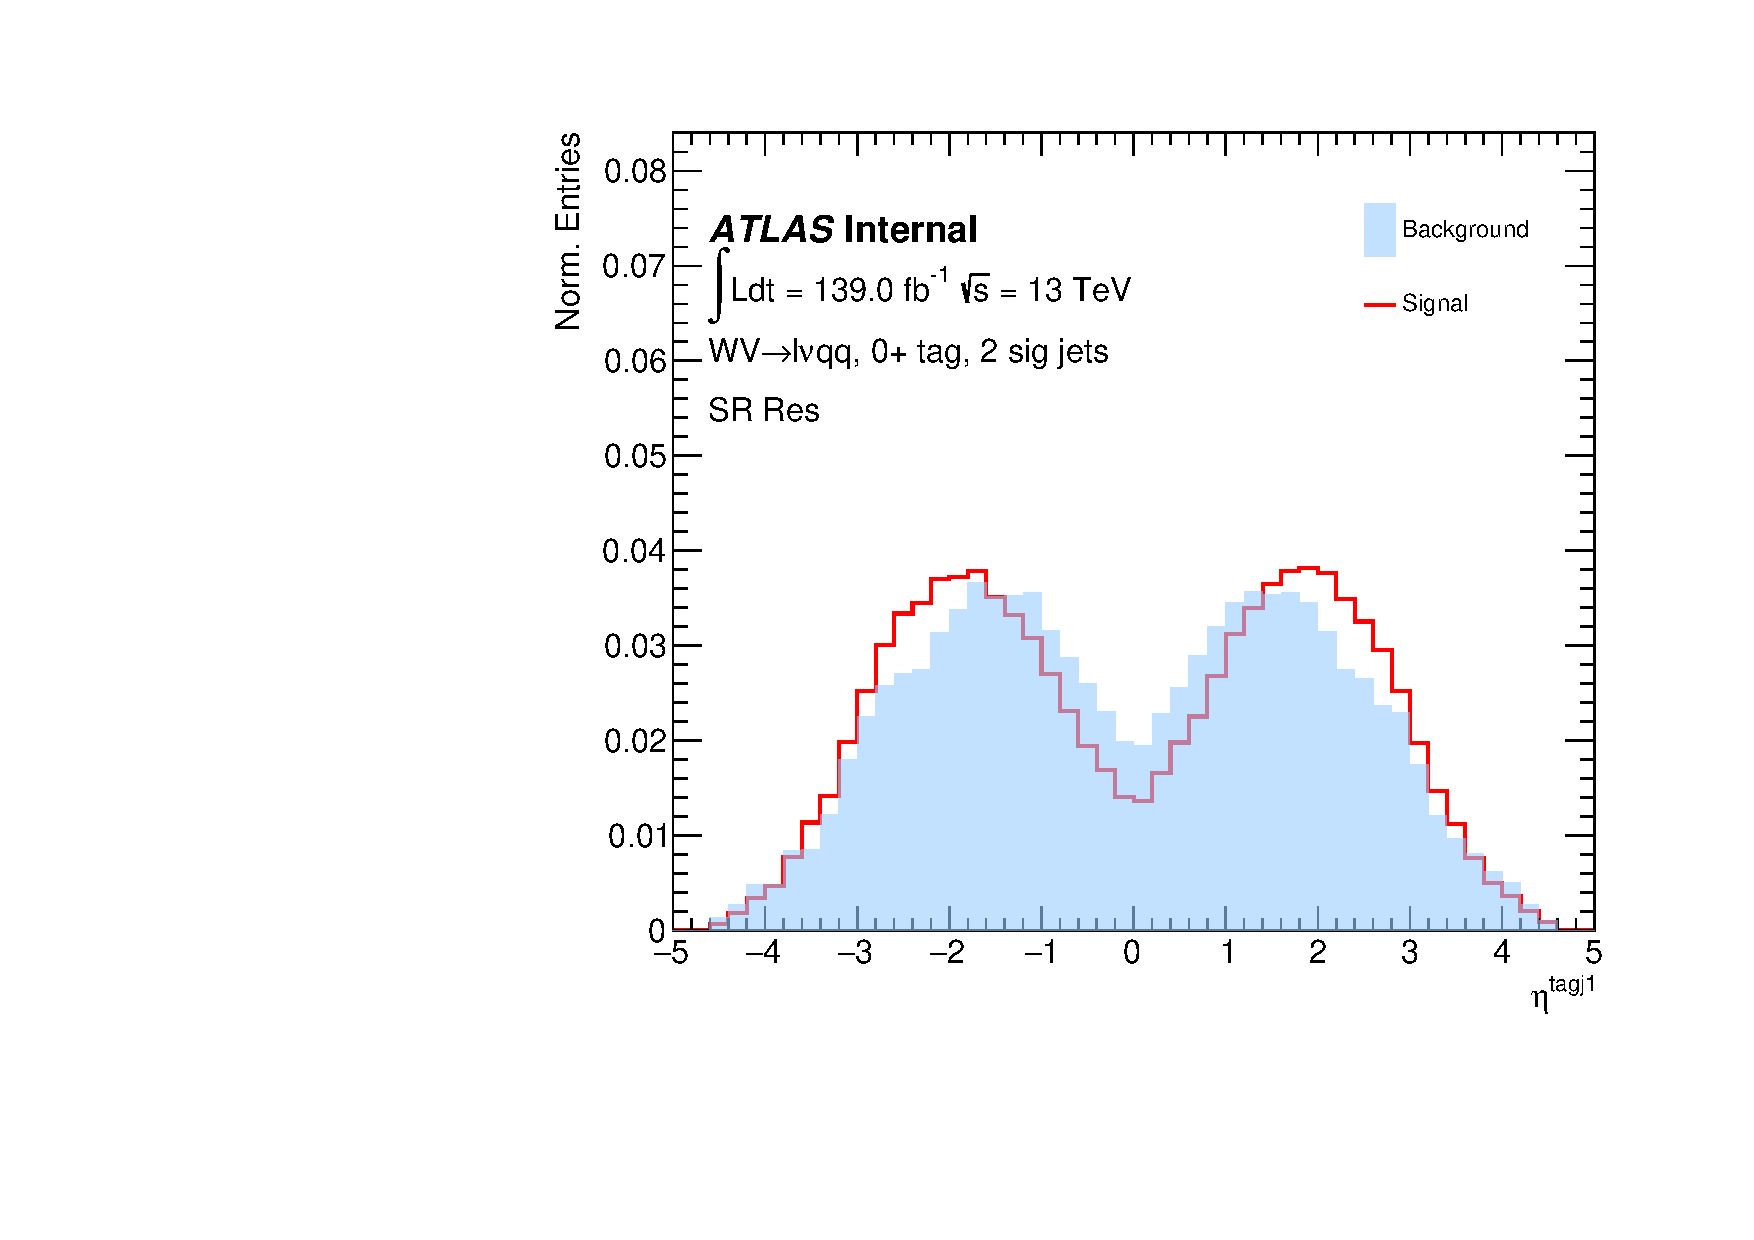
\includegraphics[width=0.3\textwidth]{figures/ml_dnn/variables/SR_Res/norm_plot_resolved_tagJ1_eta.pdf}}\quad
  \subfloat[]{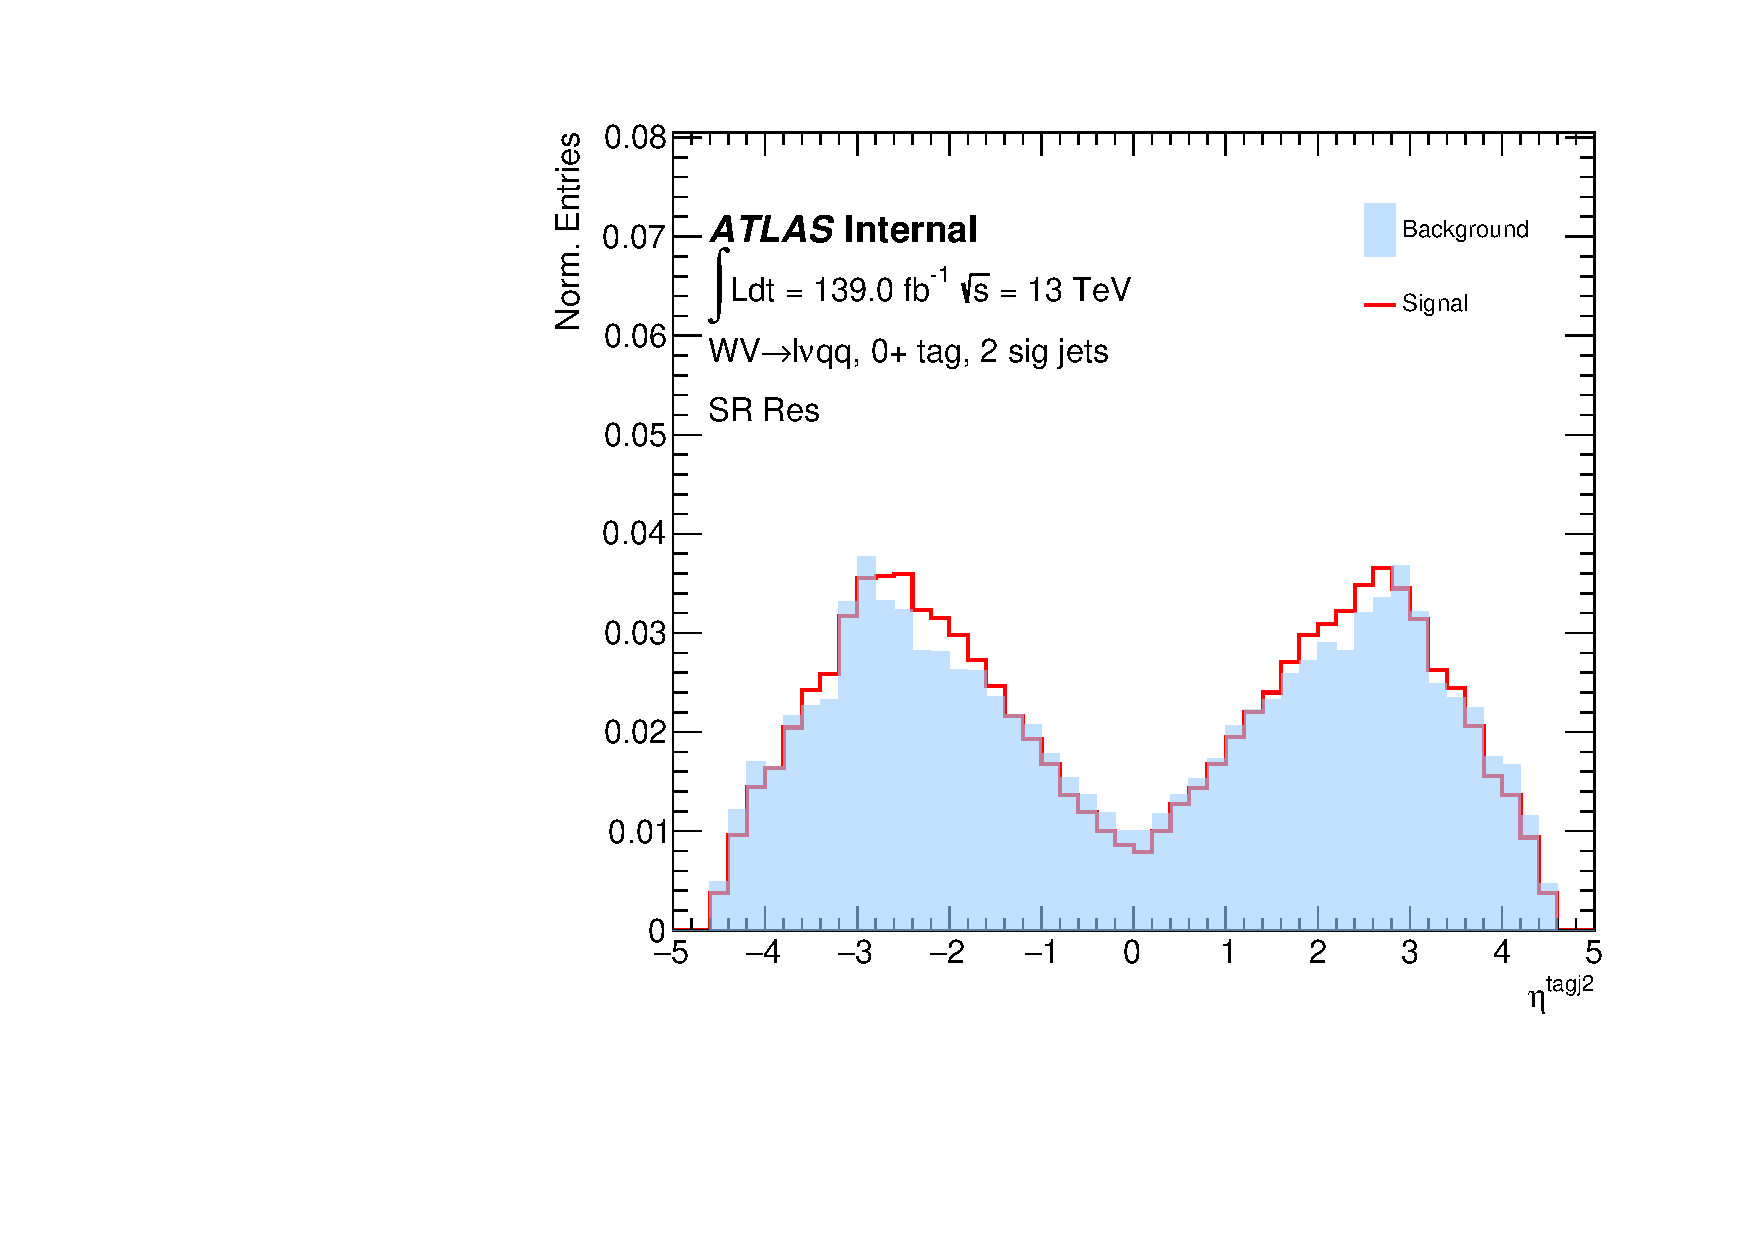
\includegraphics[width=0.3\textwidth]{figures/ml_dnn/variables/SR_Res/norm_plot_resolved_tagJ2_eta.pdf}}
  
  % Row 5
  \subfloat[]{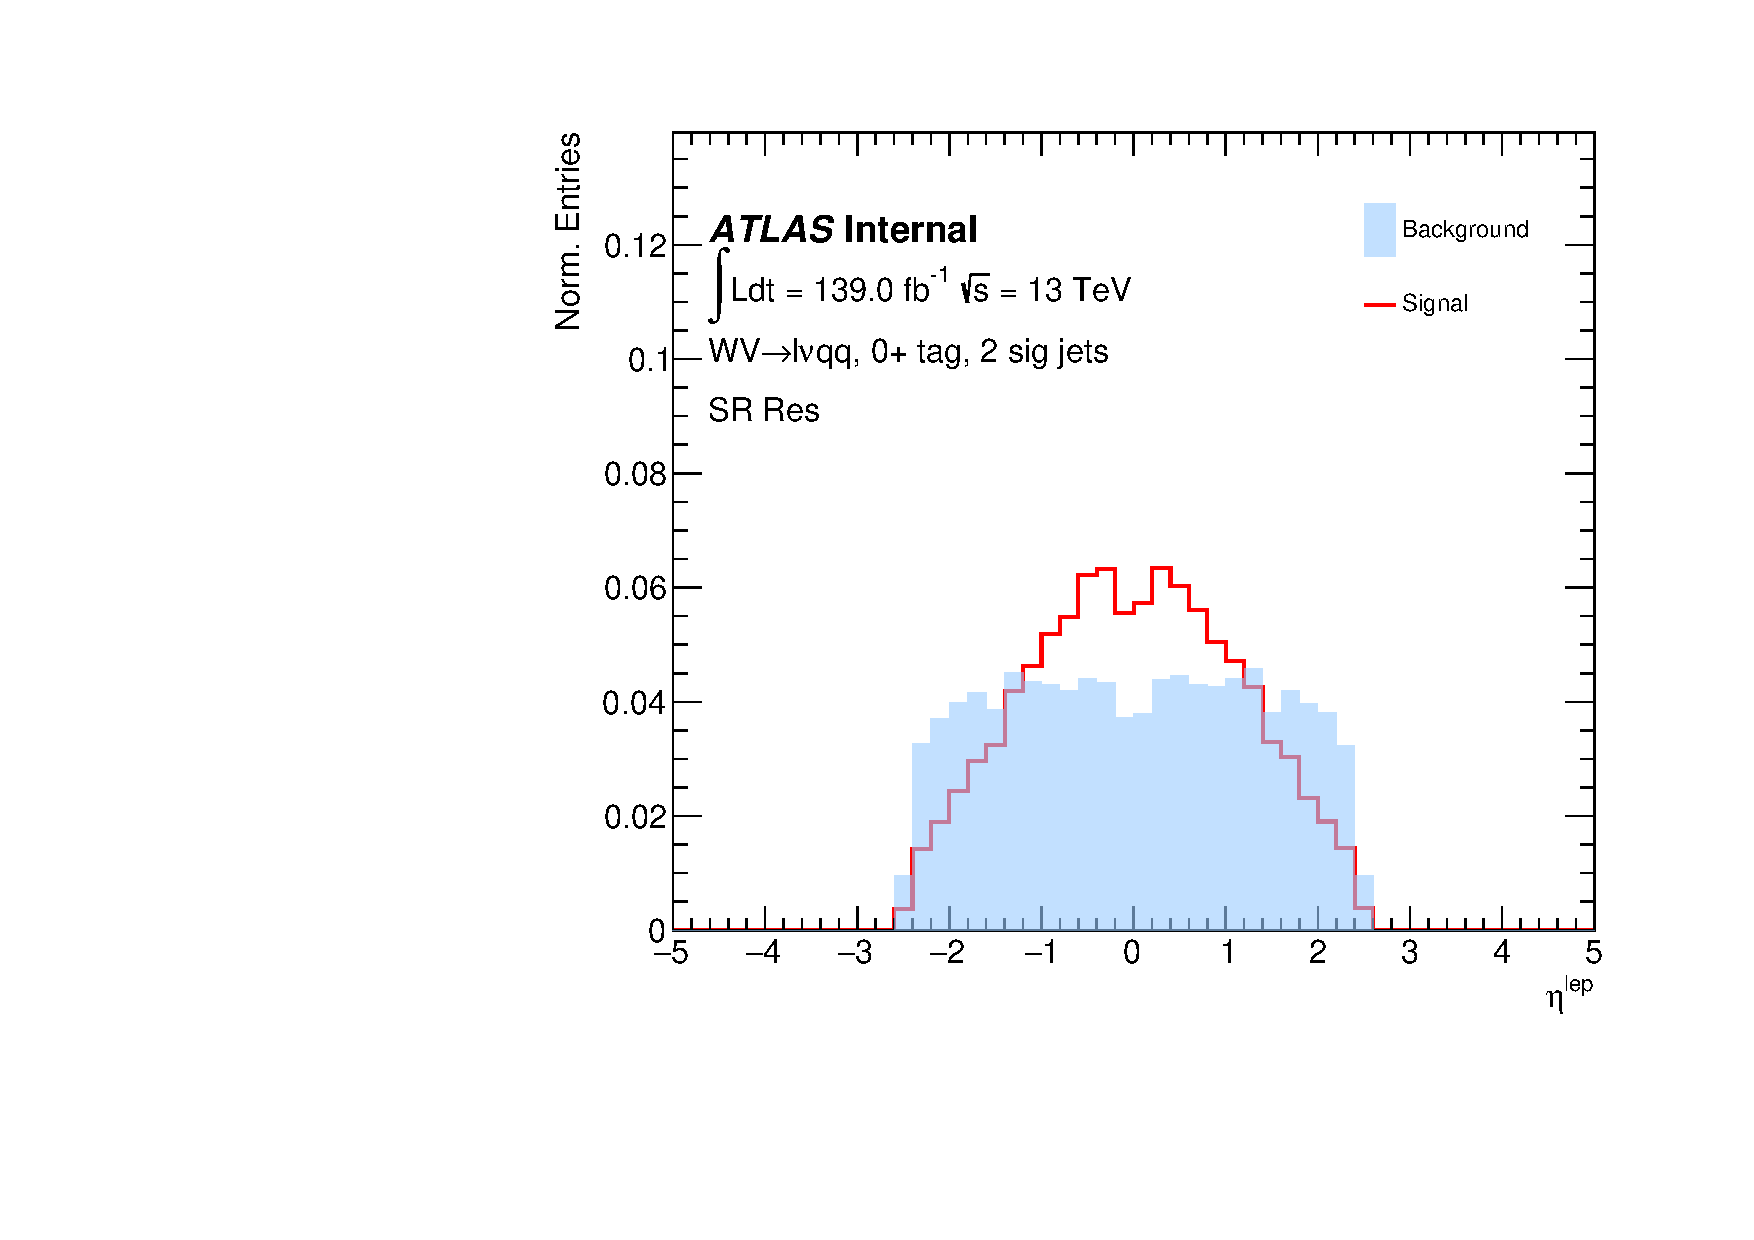
\includegraphics[width=0.3\textwidth]{figures/ml_dnn/variables/SR_Res/norm_plot_lep_eta.pdf}}\quad
  \subfloat[]{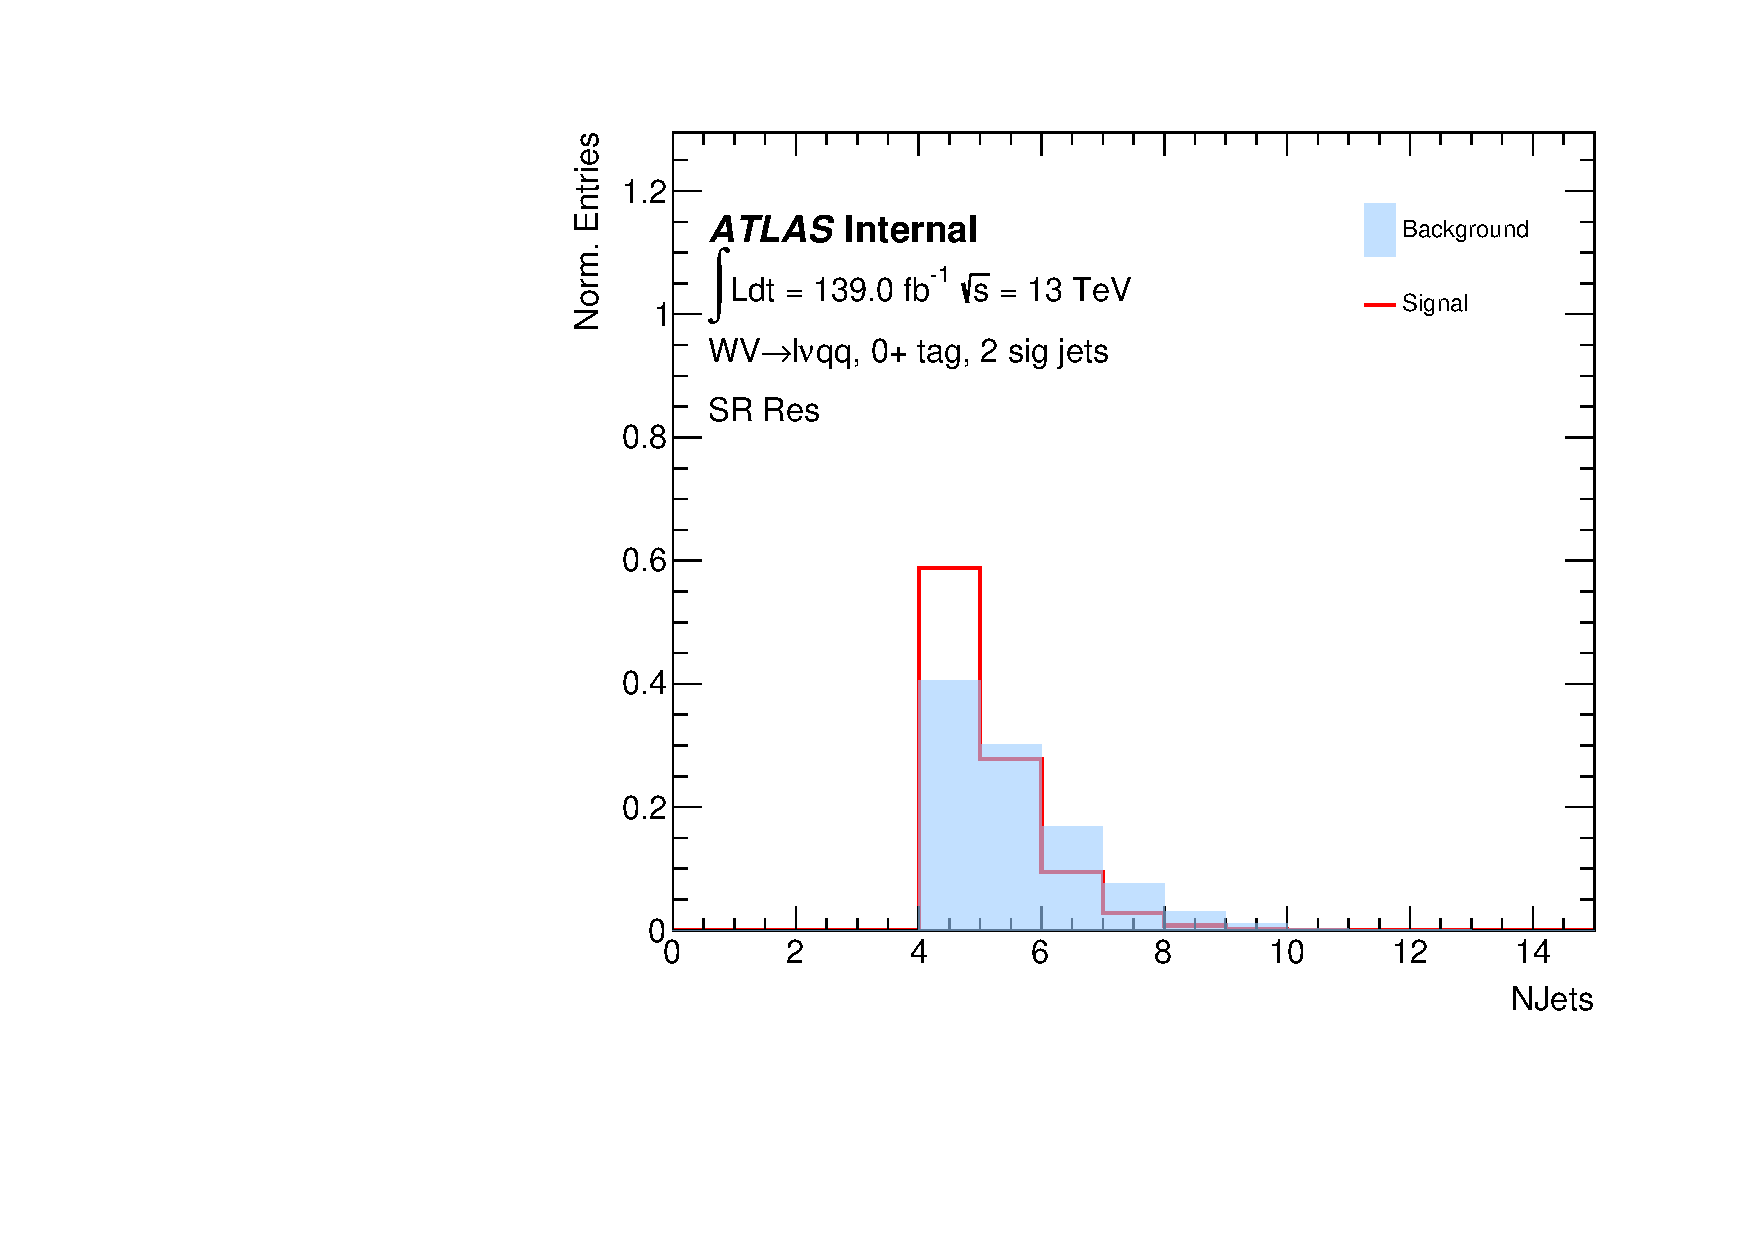
\includegraphics[width=0.3\textwidth]{figures/ml_dnn/variables/SR_Res/norm_plot_NJets.pdf}}\quad
  \subfloat[]{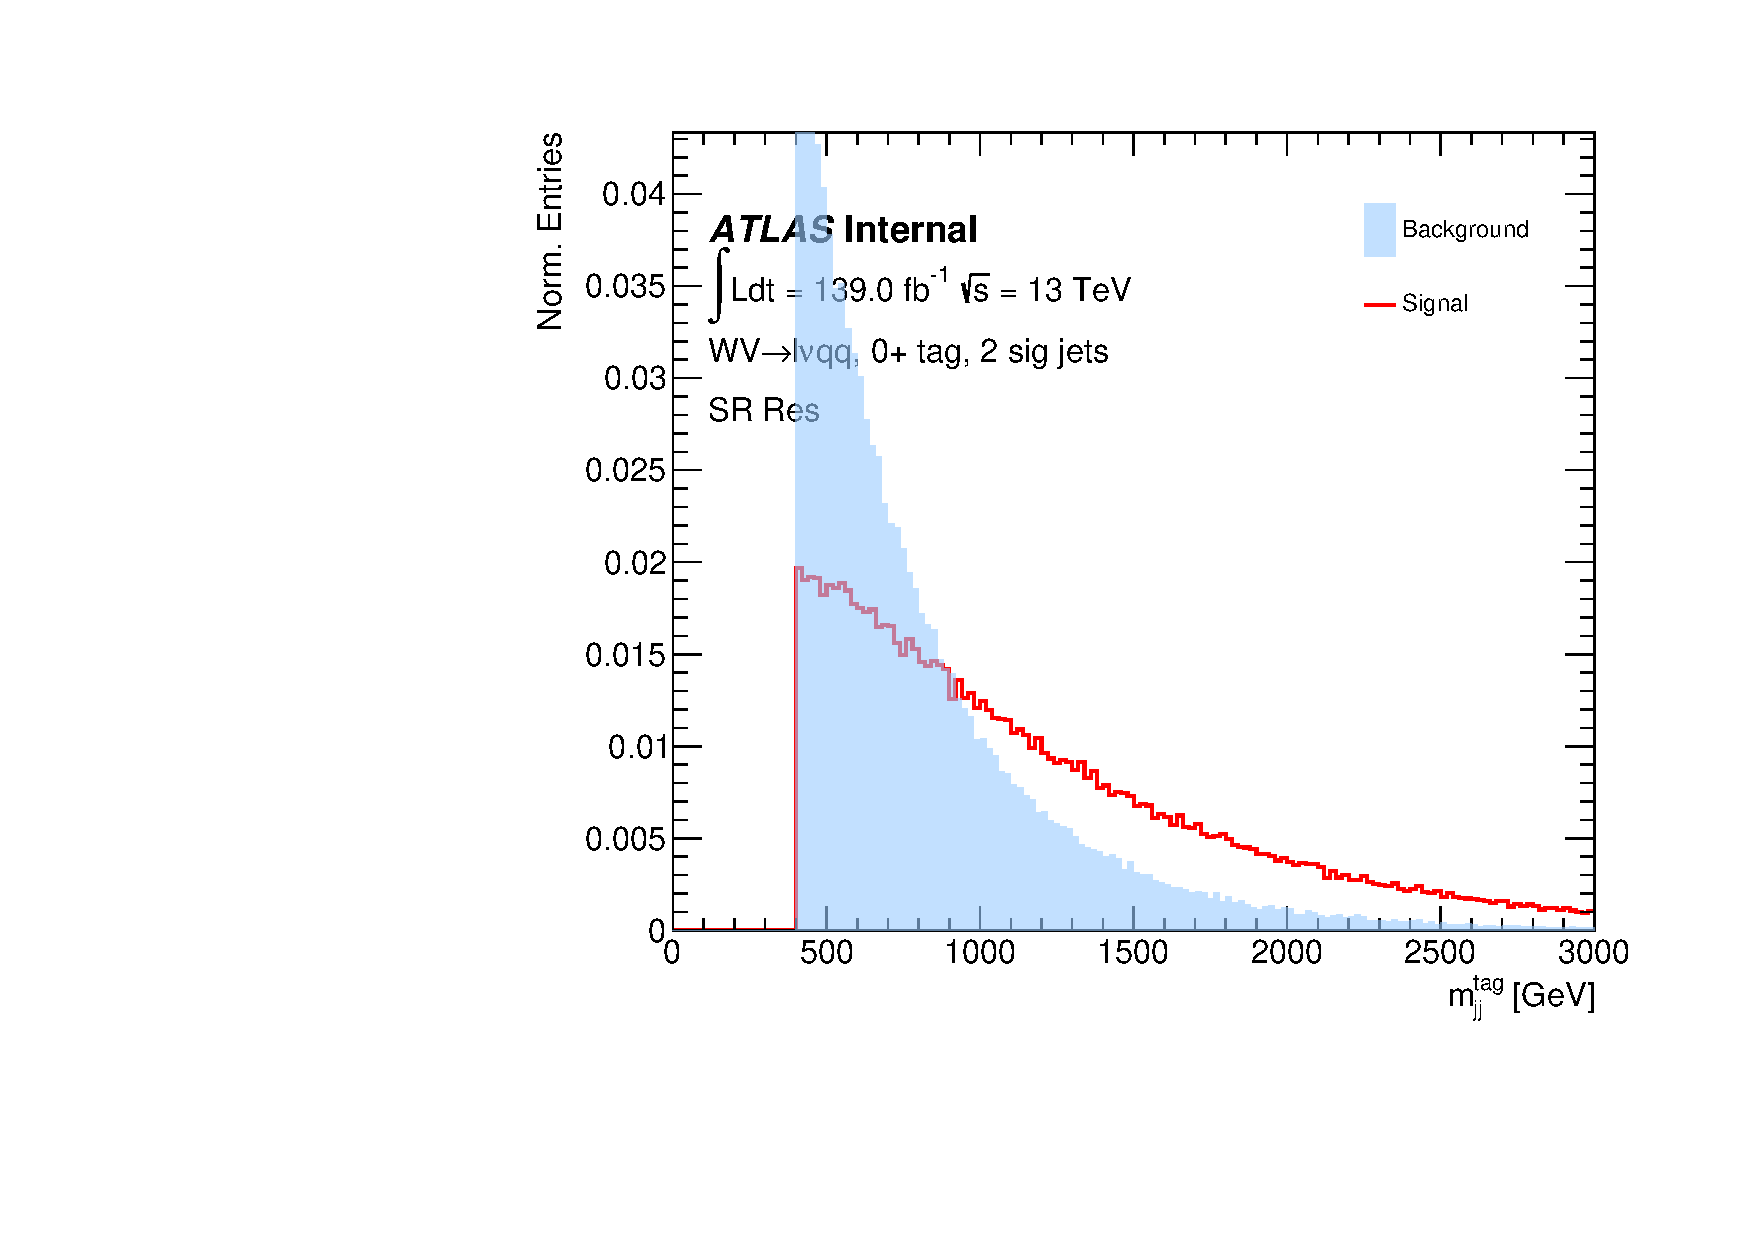
\includegraphics[width=0.3\textwidth]{figures/ml_dnn/variables/SR_Res/norm_plot_resolved_tagMjj.pdf}}
  
  % Row 6
  \subfloat[]{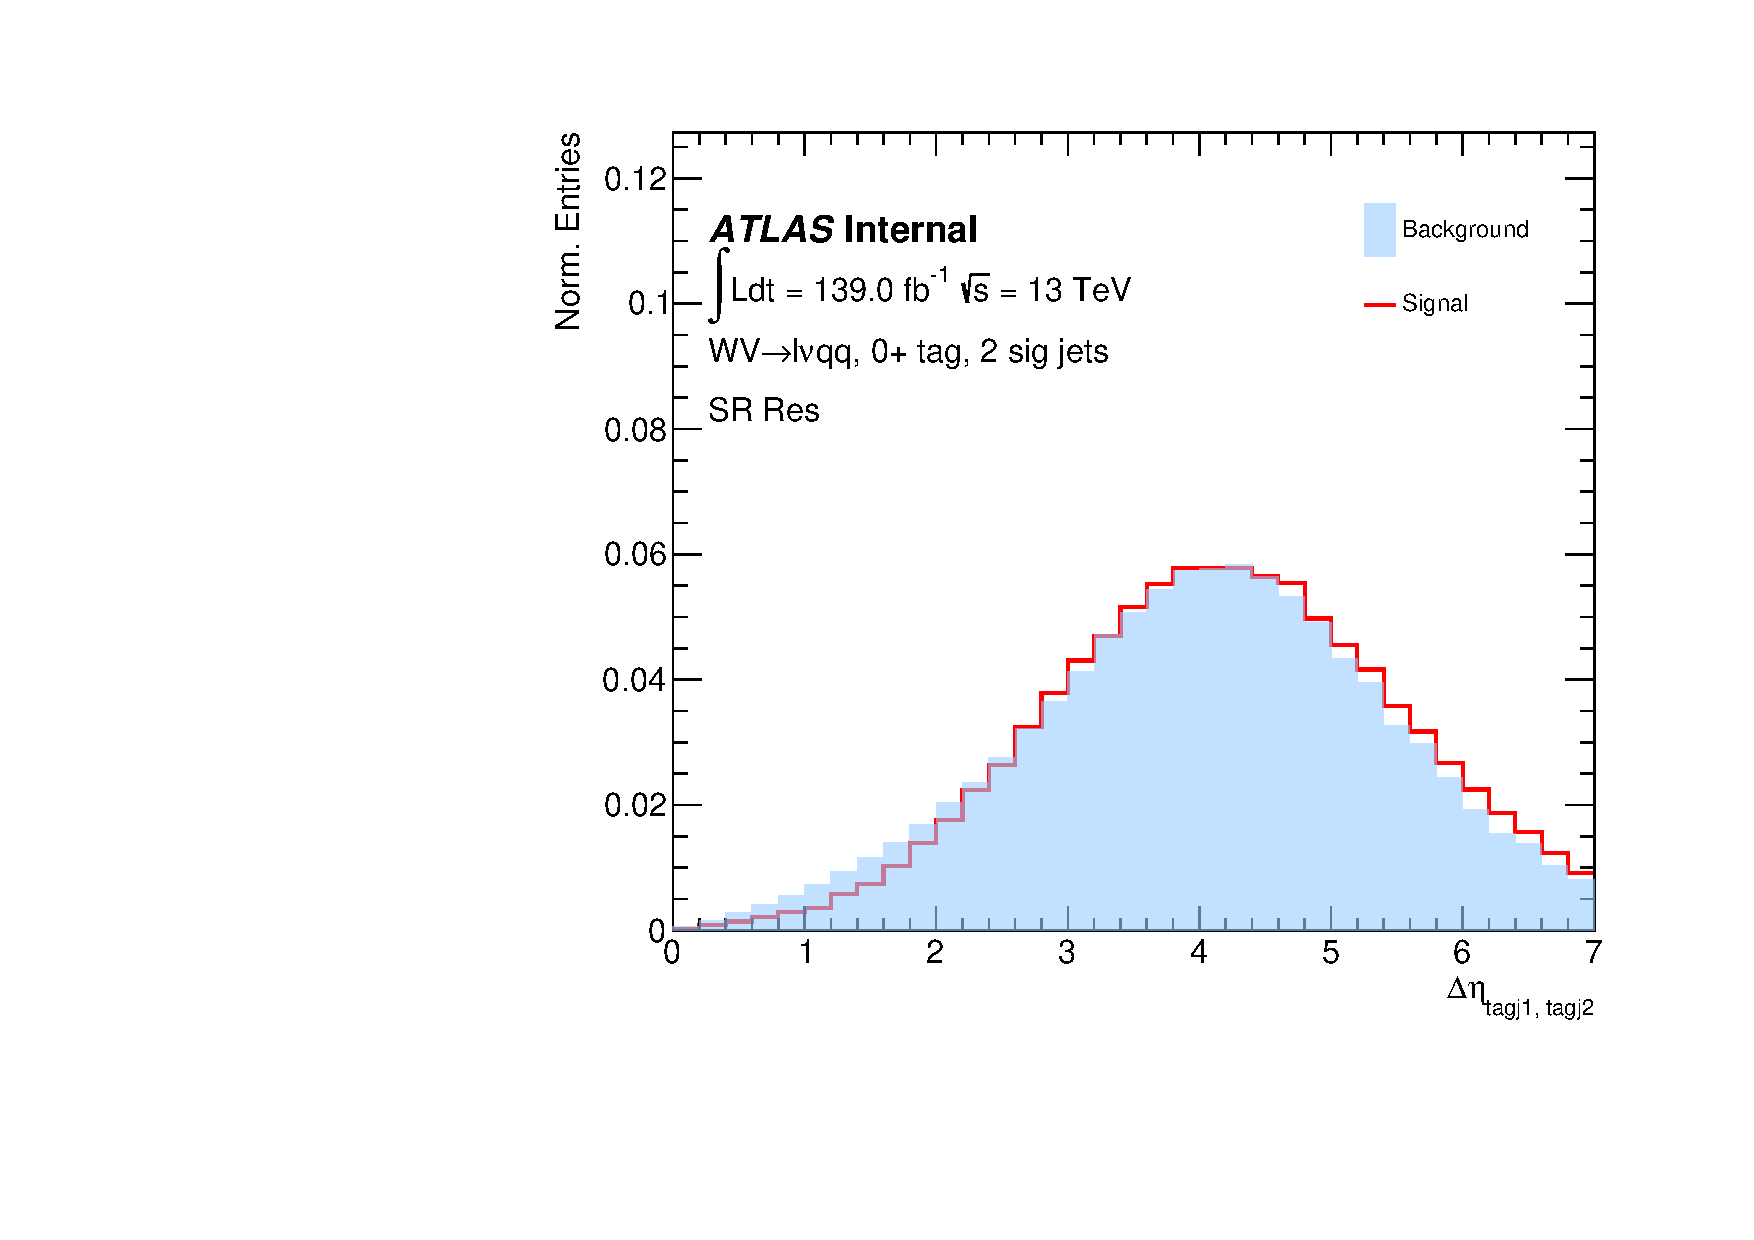
\includegraphics[width=0.3\textwidth]{figures/ml_dnn/variables/SR_Res/norm_plot_resolved_tagJdEta.pdf}}\quad
  \subfloat[]{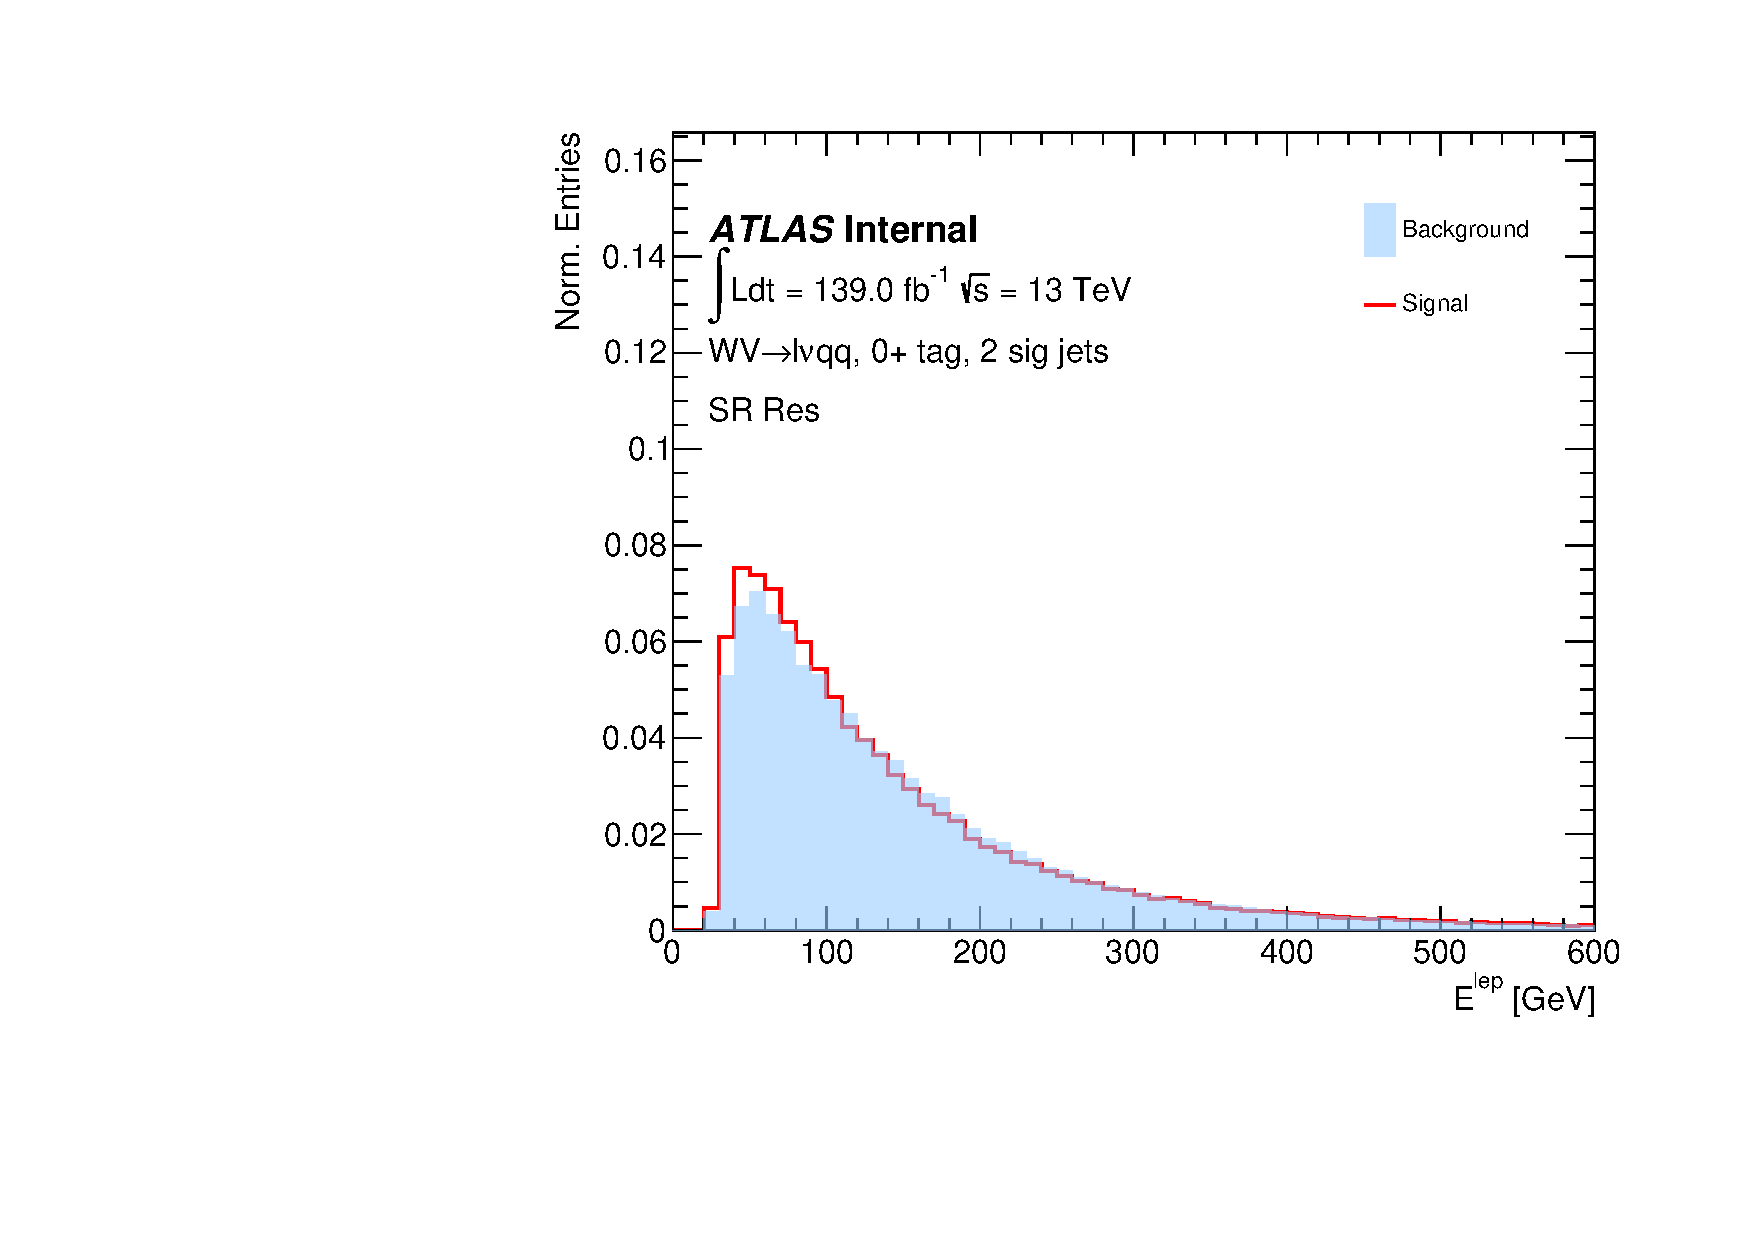
\includegraphics[width=0.3\textwidth]{figures/ml_dnn/variables/SR_Res/norm_plot_lep_e.pdf}}
  
  \caption{Distributions of input variables in the Resolved SR (Continued)}
  \label{fig:res_inputs-part2}
\end{figure}


\clearpage
\section{Trainings and Validations}
\label{trainings_and_validations}

We train separate DNN models for the merged and resolved categories. In the merged category, a single model is trained using events from both high and low purity SRs, whereas the resolved category uses its own dedicated model. For each category, the MC sample is divided into two parts: one for training and the other for validation. Within this framework, signal EW $VV+jj$ events are labeled as ``1'' and background events as ``0''.

The loss function employed is binary cross-entropy, which is well-suited for models that output binary labels, as demonstrated in Figure~\ref{fig:LossAndAccuracy}. Experiments with Adaptive Moment Estimation (Adam) and Stochastic Gradient Descent (SGD) optimizers reveal a preference for SGD due to its effectiveness in fine-tuning the distribution of DNN scores, likely attributed to its more consistent convergence behavior in our specific application.

%%%k-fold
%In this analysis, we employ the k-fold cross-validation method to fully leverage our MC samples, ensuring an unbiased evaluation of performance. 
%We utilize a 5-fold cross-validation strategy. This approach divides the dataset into 5 equally sized parts(or folds), then the DNN is trained and validated 5 times. 
%During each of the five iterations, four folds are used for training the model, while the remaining fold serves as the validation set. 
%This cyclical process ensures that every MC event in the SRs is used for both training and validation across the iterations.
%Figure \ref{fig:kfoldValidations} provides a clear indication of the DNN approach's reliability across different subsets of the dataset.

In this analysis, we employ the k-fold cross-validation method to fully leverage our MC samples, ensuring an unbiased evaluation of model performance. We utilize a 5-fold cross-validation strategy, which divides the dataset into five equally sized parts (or folds). The DNN is trained and validated five times, using a cyclical process. During each iteration, four folds are used for training the model, while the remaining fold serves as the validation set. This approach ensures that every MC event in the Signal Regions (SRs) is used for both training and validation across the iterations, thereby enhancing the robustness and generalizability of our model. Figure~\ref{fig:kfoldValidations} provides a clear indication of the reliability of the DNN approach across different subsets of the dataset.

For practicality and reliability, I implement a 2-fold cross-validation method for the DNN approach. The complete MC sample is evenly divided into two parts: one for training and the other for validation. 
The consistent performance across these datasets, highlighted in Figure~\ref{fig:ROCValidations}, indicates an absence of training set bias. This consistency ensures the model's robustness and unbiased evaluation.

Figure~\ref{fig:1lepDNN_performance} demonstrates the effective separation between signal and background in the DNN distributions for both merged and resolved regimes. Figure~\ref{fig:1lepDNNoutputs} presents the distributions of DNN scores across all three signal regions, with some data bins partially blinded.

%For practicality and reliability, I employs a 2-fold cross-validation method for the DNN approach. The complete MC sample is evenly divided into training and testing datasets. The consistent performance between these datasets, highlighted in Figure \ref{fig:ROCValidations}, indicates no training set bias. 
%Figure~\ref{fig:1lepDNN_performance} demonstrates the effective separation between signal and background in the DNN distribution for both merged and resolved regimes. Figure~\ref{fig:1lepDNNoutputs} presents the DNN score distributions across all three signal regions, featuring partially blinded data bins.

\begin{figure}[ht]
      \centering
       \subfloat[\emph{Loss curve}]{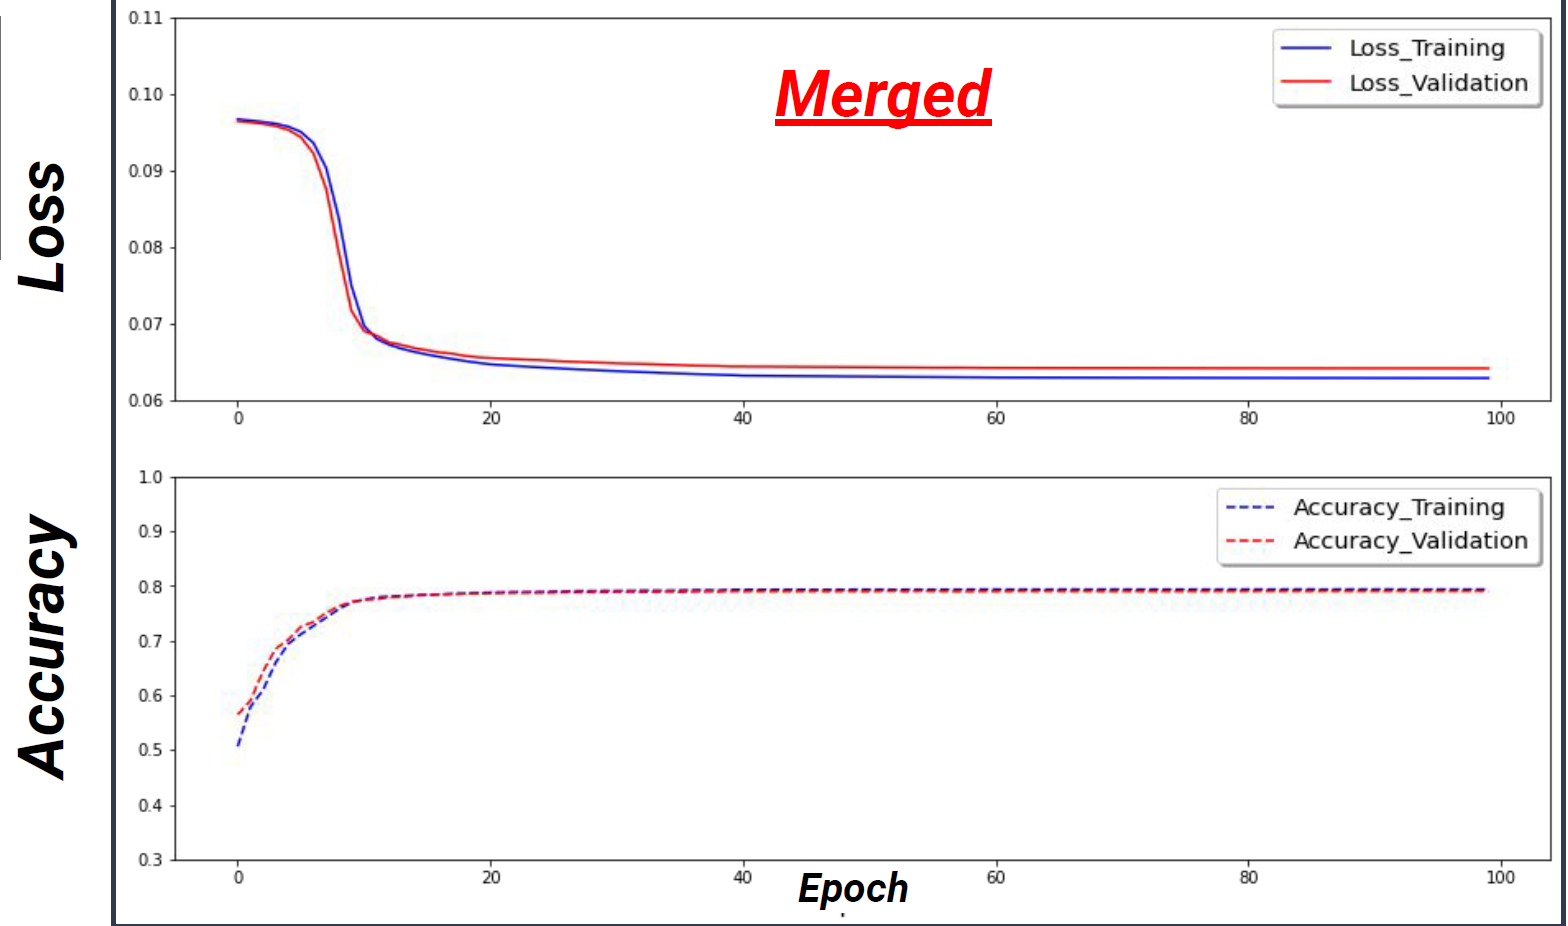
\includegraphics[width=0.45\textwidth]{figures/ml_dnn/loss_mer.png}}
       \subfloat[\emph{Loss curve}]{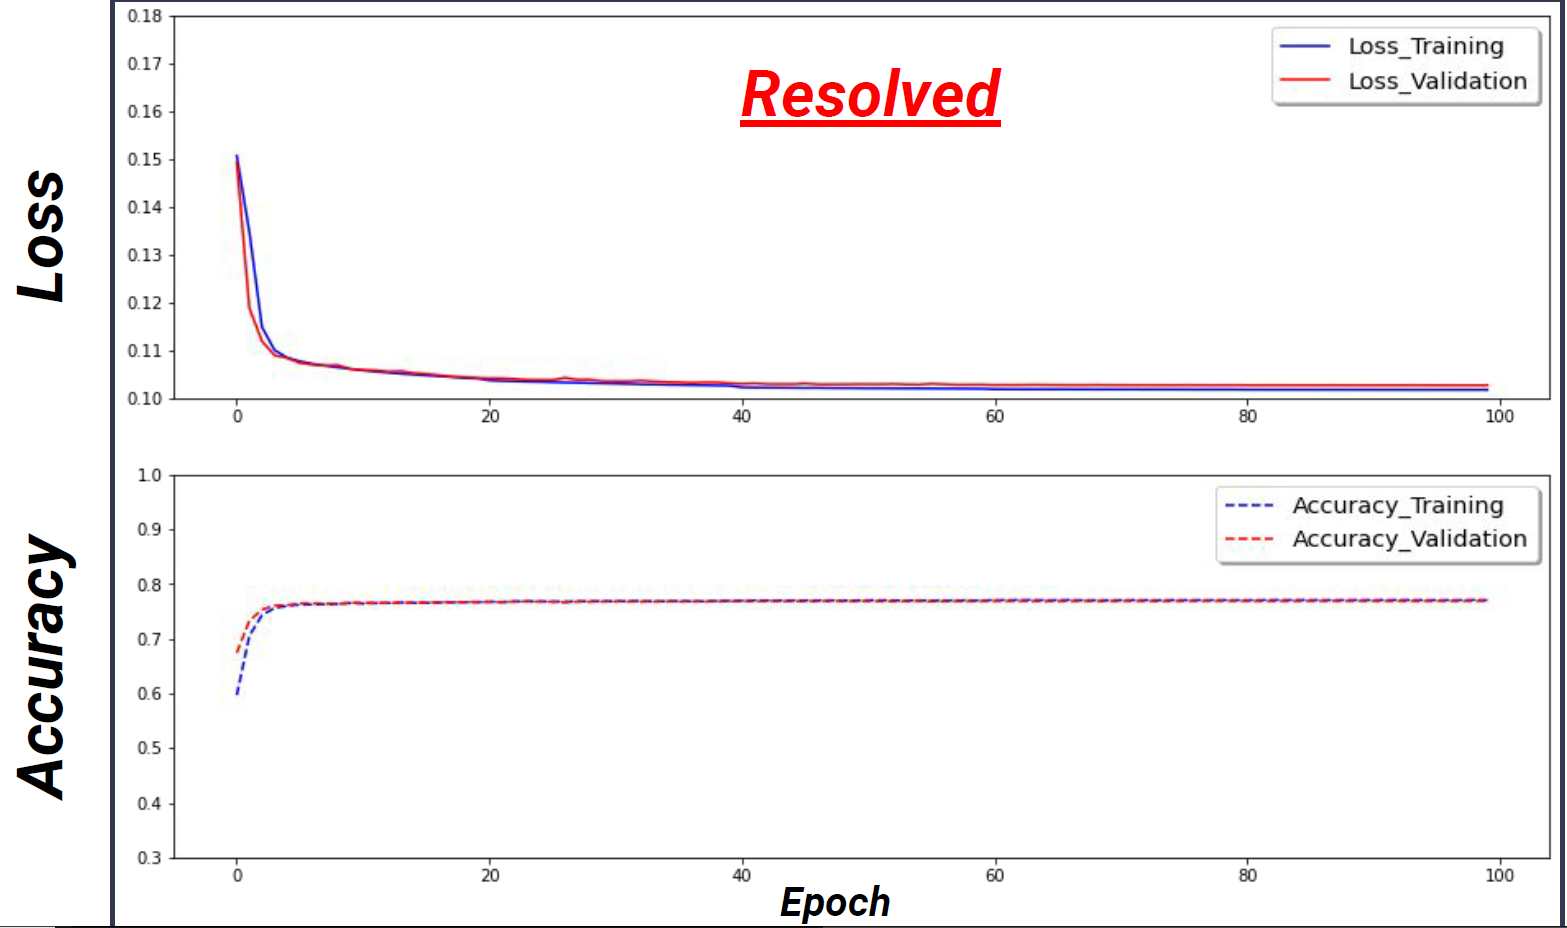
\includegraphics[width=0.45\textwidth]{figures/ml_dnn/loss_res.png}}
       \caption{Trainings for the DNN models in the merged and resolved regimes.}
       \label{fig:LossAndAccuracy}
\end{figure}

\begin{figure}[ht]
      \centering
       \subfloat[\emph{ROC curve}]{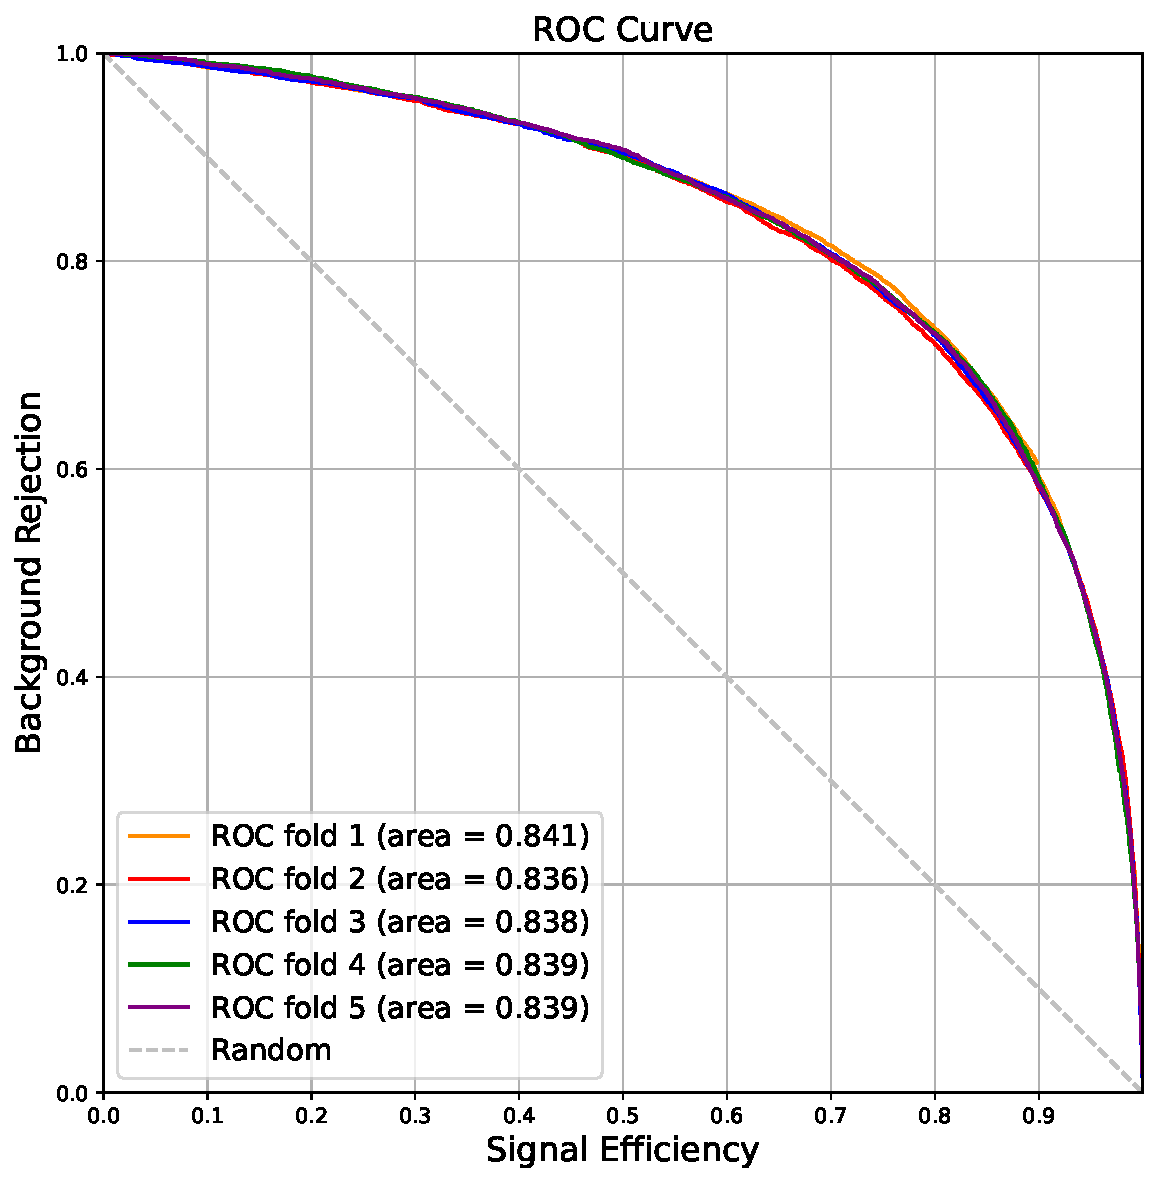
\includegraphics[width=0.45\textwidth]{figures/ml_dnn/kfold/roc_curve_mer.pdf}}
       \subfloat[\emph{ROC curve}]{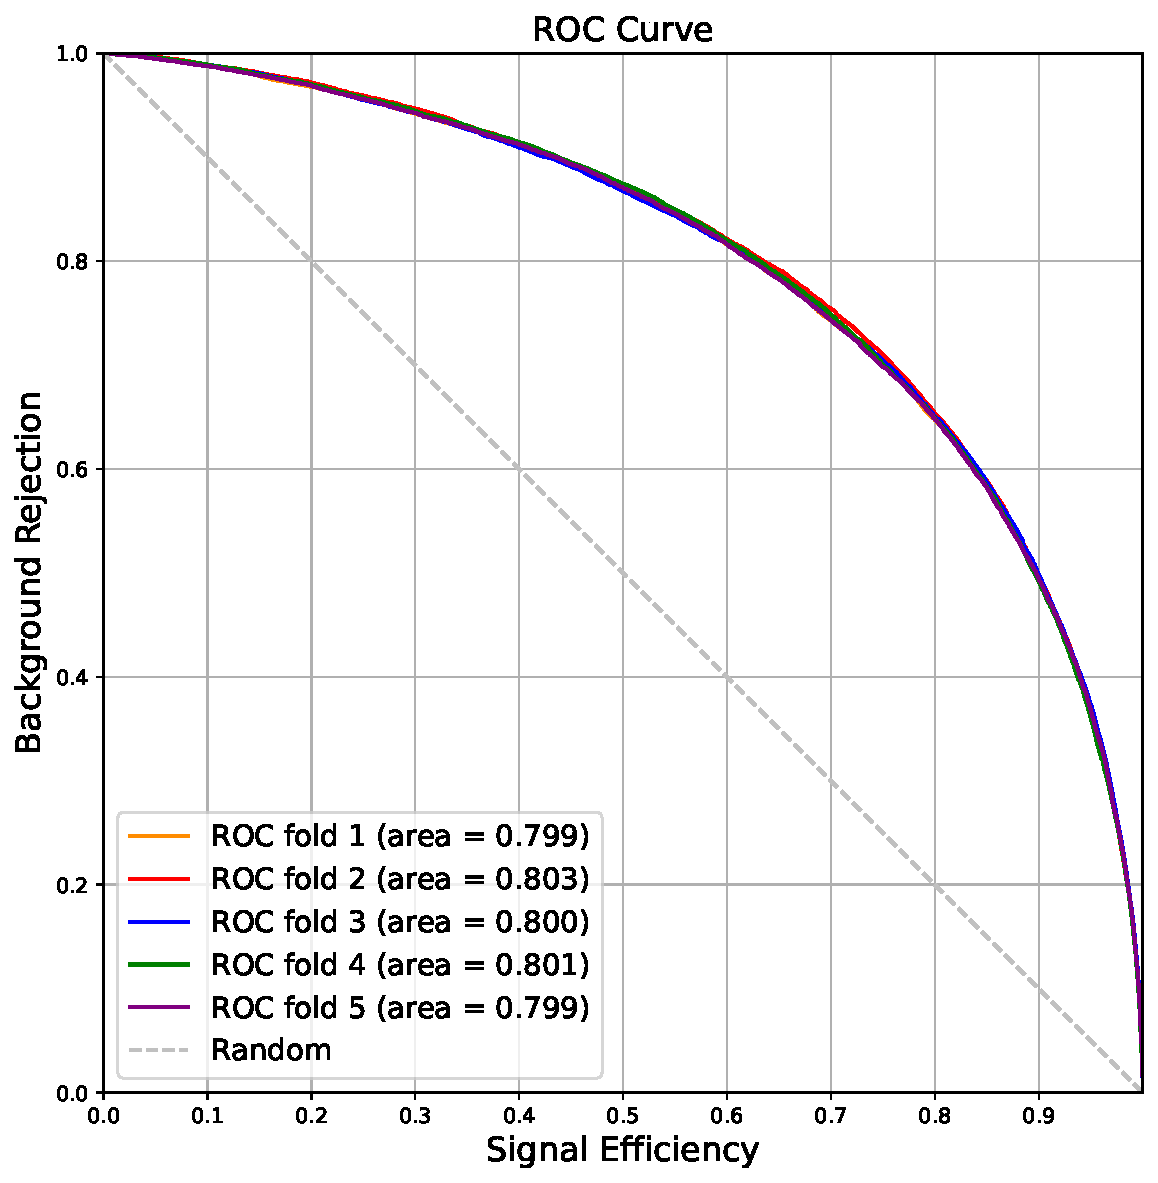
\includegraphics[width=0.45\textwidth]{figures/ml_dnn/kfold/roc_curve_res.pdf}}
       \caption{K-fold cross-validation for the DNN model trained in the merged and resolved regimes.}
       \label{fig:kfoldValidations}
\end{figure}


\begin{figure}[ht]
      \centering
       \subfloat[\emph{ROC curve}]{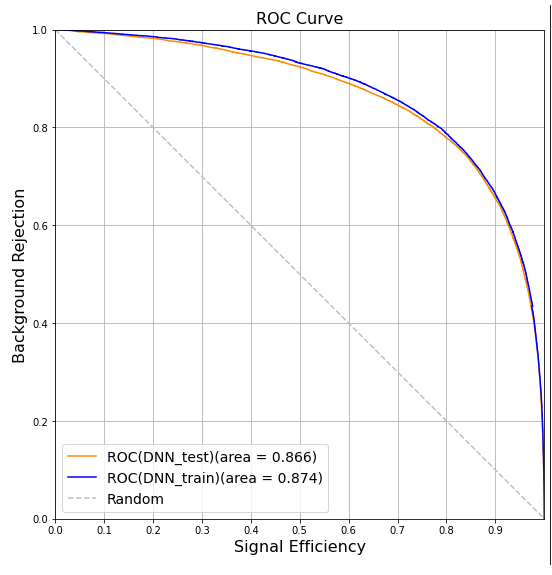
\includegraphics[width=0.45\textwidth]{figures/ml_dnn/roc_mer.png}}
       \subfloat[\emph{ROC curve}]{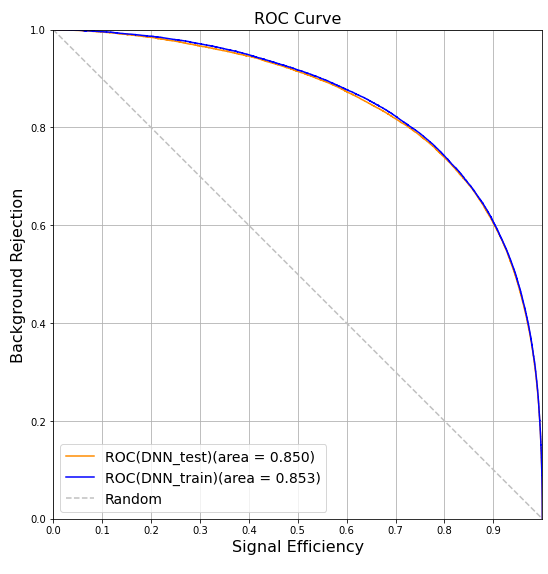
\includegraphics[width=0.45\textwidth]{figures/ml_dnn/roc_res.png}}
       \caption{Validation for the DNN model trained in the merged and resolved regimes.}
       \label{fig:ROCValidations}
\end{figure}

\begin{figure}[ht]
      \centering
       \subfloat[\emph{DNN Merged}]{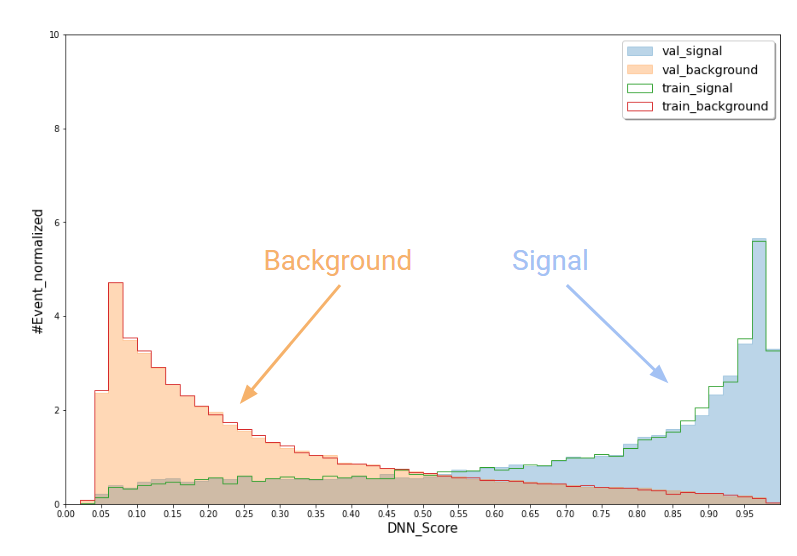
\includegraphics[width=0.45\textwidth]{figures/ml_dnn/dnn_dist/dnn_norm_mer.PNG}}
       \subfloat[\emph{DNN Resolved}]{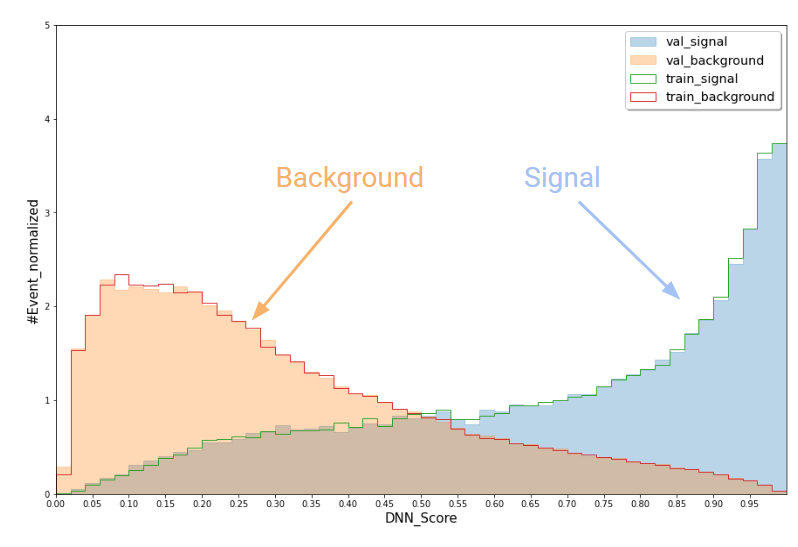
\includegraphics[width=0.45\textwidth]{figures/ml_dnn/dnn_dist/dnn_norm_res.PNG}}
       \caption{Performance for the DNN model trained in the merged and resolved regimes.}
       \label{fig:1lepDNN_performance}
\end{figure}

\begin{figure}[ht]
 \begin{center}
  \subfloat[DNN HP]{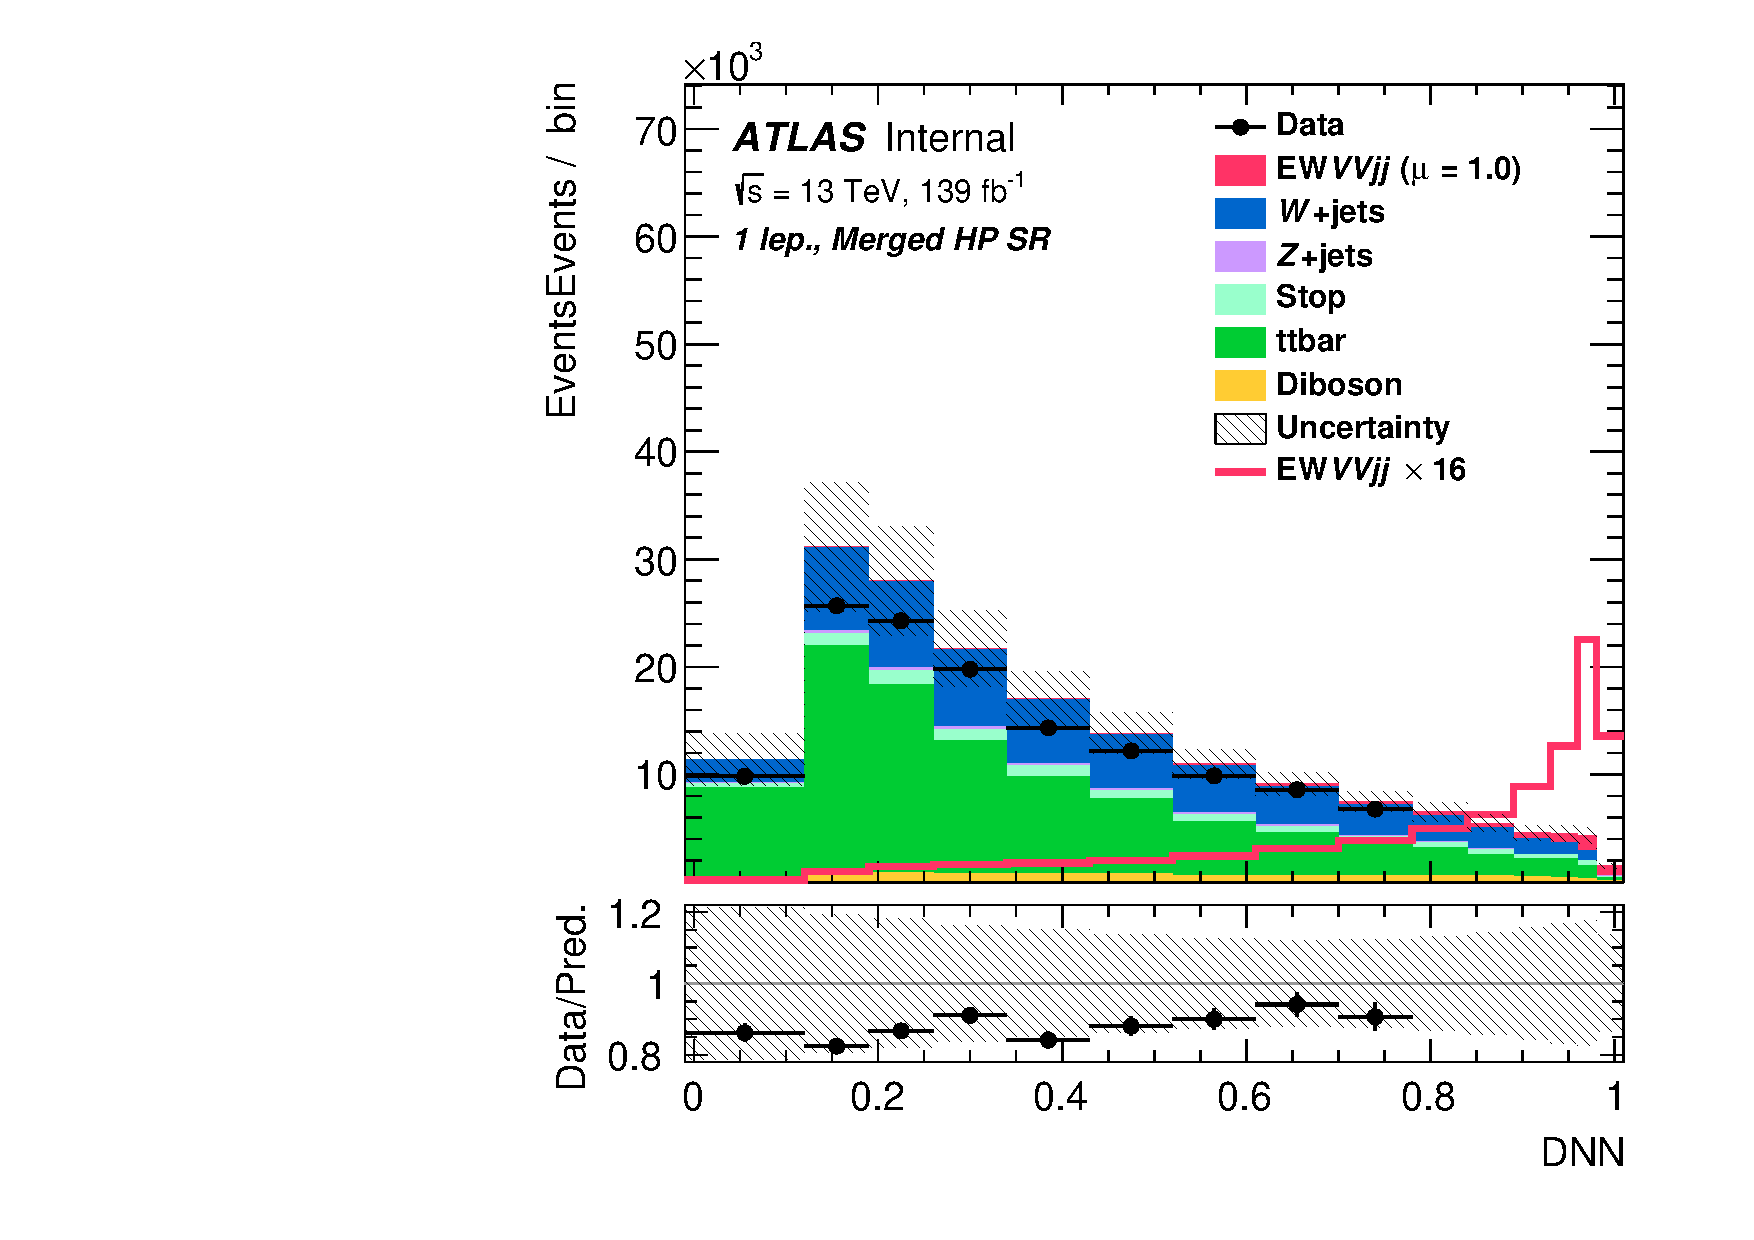
\includegraphics[width=0.3\textwidth]{figures/ml_dnn/Region_distDNN_DSRVBSHP_BMin0_J0_incJet1_L1_T0_incFat1_Y6051_incTag1_Fat1_Prefit.pdf}}
  \subfloat[DNN LP]{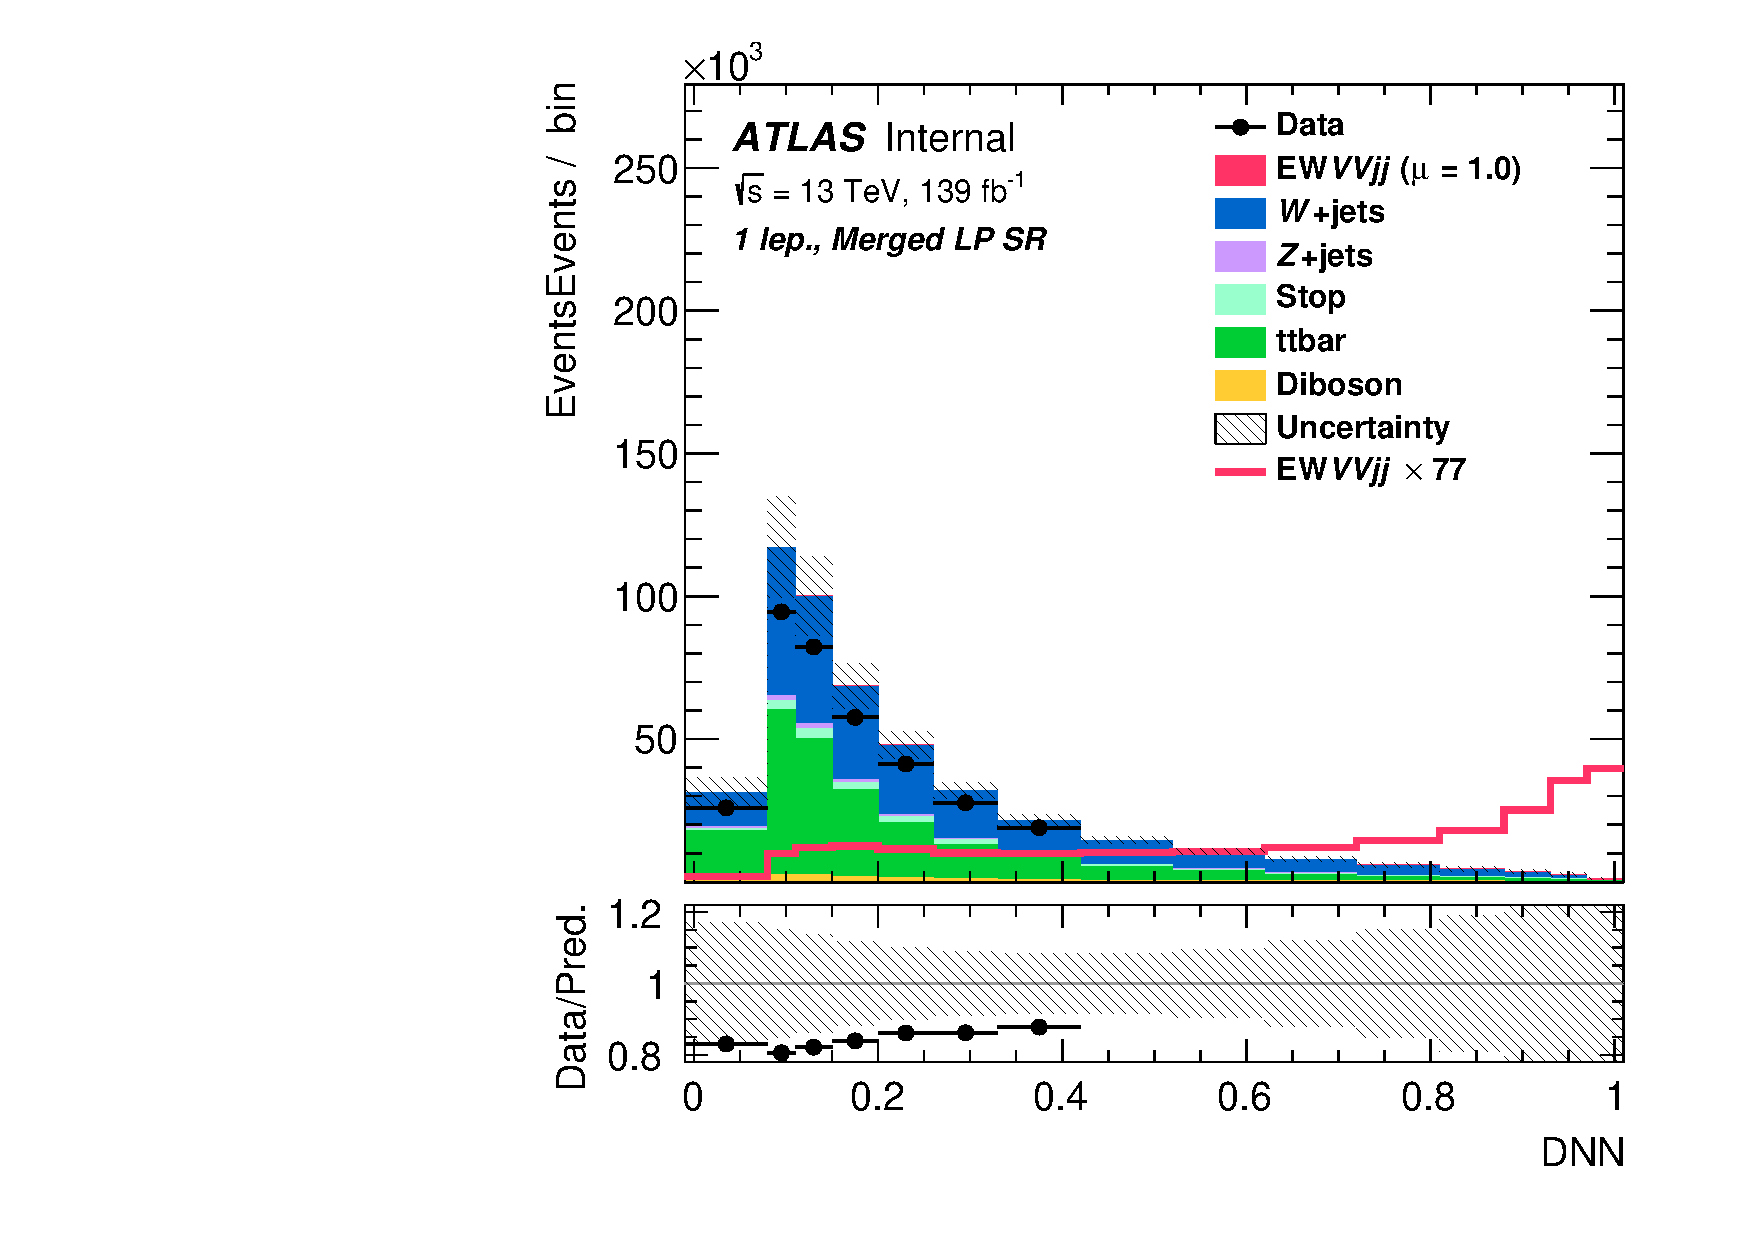
\includegraphics[width=0.3\textwidth]{figures/ml_dnn/Region_distDNN_DSRVBSLP_BMin0_J0_incJet1_L1_T0_incFat1_Y6051_incTag1_Fat1_Prefit.pdf}}
  \subfloat[DNN Res]{\includegraphics[width=0.3\textwidth]{figures/ml_dnn/Region_distDNN_DSRVBSTight_BMin0_T0_Y6051_incTag1_J2_L1_incJet1_Prefit.pdf}}
  \caption{DNN score distributions for the high purity merged, low purity merged, and resolved signal regions.}
 \label{fig:1lepDNNoutputs}
 \end{center}
\end{figure}


